% !TeX program = lualatex
\documentclass[a4paper,12pt,landscape,british,oneside]{memoir}

\usepackage{microtype} % micro adjustments to font spacing does actually reduce overfull hboxes

\usepackage{ifthen}
\newboolean{printVersion}\setboolean{printVersion}{true}
\newboolean{answersAtEnd}\setboolean{answersAtEnd}{true}
\newboolean{notesAtEnd}\setboolean{notesAtEnd}{false}
\newboolean{compressBibliography}\setboolean{compressBibliography}{false}
\newboolean{showUnclearedCopyright}\setboolean{showUnclearedCopyright}{true}
\newboolean{a5Target}\setboolean{a5Target}{false}

% 0.6180339887498948482
\newcommand{\jdraftnumber}{7.6}
\newcommand{\jPublicationYear}{2025}




\usepackage[british]{babel}\usepackage{csquotes}

% for main body text, might reset for bibliography
\settypeblocksize{*}{10cm}{1.6}
\setulmarginsandblock{2cm}{2cm}{*}
\setlrmarginsandblock{2cm}{15cm}{*}
\checkandfixthelayout
% \usepackage[showframe, pass]{geometry} 

\chapterstyle{dash}


\usepackage{amsmath} % \cfrac
\usepackage{amsfonts}
\usepackage{amsthm}  % \proof
\usepackage{amssymb} %R
\usepackage{overpic} % \overpic for cover page
\usepackage{textpos} % \textblock for cover page
\usepackage{gensymb}% \degree

\usepackage{mathtools} % intertext
\renewcommand{\implies}{\Rightarrow}

\DeclareMathOperator\sign{sign} % from amsmath

\usepackage{todonotes} % consider fixme instead - would probably be faster but may not work out of the box

\usepackage{fontspec}
\usepackage{CormorantGaramond} % by default using lining not oldstyle numnbers; seems to get those from Latin Modern...
\usepackage[scaled=0.9]{gillius2} % sets only sffamily; use \usepackage[sfdefault]{gillous} to set rm text too 

\usepackage{xcolor}
\definecolor{CylinderColour}{rgb}{0.86, 0.86, 0.64}
\definecolor{parastichy1}{rgb}{0.71, 0.3214, 0.27}
\definecolor{parastichy2}{rgb}{0.46, 0.2947, 0.591}
\definecolor{parastichy3}{rgb}{0.45, 0.54, 0.24}
\definecolor{parastichy4}{rgb}{0.95, 0.94,0.94}
\definecolor{parastichy5}{rgb}{0.21, 0.1875, 0.15}
\newcommand{\jHeadingColour}{\color{parastichy1}}
\newcommand{\jEmphasisColour}{\color{parastichy1}}
\newcommand{\jLinkColour}{\color{parastichy2}}
\newcommand{\jBodyTextColour}{\color{black}}

%\addtodef\chaptitlefont{}{\jHeadingColour}\renewcommand\colorchapnum{\color{ared}}

% chapter number and name
\addtodef\chapnumfont{}{\jHeadingColour}
\renewcommand*{\chaptitlefont}{\huge\bfseries\centering\jHeadingColour}


\setsecheadstyle{\jHeadingColour}% Set \section style
\setsubsecheadstyle{\jHeadingColour}% Set \section style
\setsecnumdepth{subsection}
\addtodef{\tocheadstart}{\color{black}}{} 
\addtoiargdef{\printtoctitle}{\color{black}}{} 


\setbeforesecskip{-\onelineskip}
\setaftersecskip{\onelineskip}

\newcommand{\mydraft}{NOT FOR PUBLICATION \jdraftnumber{}}
\renewcommand{\mydraft}{}

\newcommand{\jPage}{\jHeadingColour[\thepage]}
\makeoddfoot{plain}{\mydraft}{\jPage}{}
%\makeoddfoot{empty}{\null\vspace{2cm}\null\mydraft\jPage}{}
\makeoddfoot{empty}{}{}{}
\makeoddfoot{simple}{\mydraft}{\jPage}{simple}
\makeoddfoot{headings}{\mydraft}{\jPage}{}
\makeoddhead{headings}{}{\jHeadingColour\leftmark}{}
\makeevenhead{headings}{}{\large\jHeadingColour MATHEMATICAL PHYLLOTAXIS}{}
\makeevenfoot{headings}{}{\jPage}{}
%%%%%%%%epigraph
\setlength{\epigraphwidth}{6cm}

%%%%%%%%%%%%%%% bib 
\usepackage[backend=biber,style=ext-numeric,giveninits=true,
bibencoding=utf8,articlein=false]{biblatex}
\addbibresource{MPCite.bib} % generated by Zotero straight into this directory#
%\renewcommand*{\bibannotationprefix}{bibannotation-}

\renewbibmacro{finentry}{%
	\usebibmacro{annotation}%
		\setunit{%
		\finentrypunct
		\renewcommand*{\finentry}{}%
		\par}%
	\finentry
}

\renewbibmacro*{doi+eprint+url}{%
	\iftoggle{bbx:doi}{\printfield{doi}}{}\newunit\newblock
	\iftoggle{bbx:url}{\iffieldundef{doi}{\usebibmacro{url}}{}}{}
}

\DeclareOuterCiteDelims{cite}{\jLinkColour{\bibopenbracket}}{\jLinkColour{\bibclosebracket}}
\DeclareFieldFormat{doi}{%
	\mkbibacro{DOI}\addcolon\space
	\ifhyperref
	{\href{https://doi.org/#1}{	\jLinkColour\nolinkurl{#1}}}
	{\color{blue}\nolinkurl{#1}}}
\DeclareFieldFormat{url}{%
	\ifhyperref
	{\href{#1}{	\jLinkColour	\mkbibacro{URL}}}
	{\color{blue}\nolinkurl{#1}}}
\DeclareFieldFormat{isbn}{%
	\mkbibacro{ISBN}\addcolon\space
	\ifhyperref
		{\href{https://worldcat.org/isbn/#1}{\jLinkColour\nolinkurl{#1}}}
	{\color{blue}\nolinkurl{#1}}}

\renewbibmacro*{annotation}{\iffieldundef{annotation}{}{\printfield{annotation}}}

\ifthenelse{\boolean{printVersion}}{
\AtEveryBibitem{% 
	\clearfield{url}
	\clearfield{lang}
	\clearfield{urldate}
	\clearfield{issn}
	\clearfield{isbn}
	\clearfield{pmid}
	\clearfield{doi}
	\clearfield{visited}
}
}{% not printversion
\AtEveryBibitem{% 
	\clearfield{lang}
	\clearfield{urldate}
	\clearfield{issn}
	\clearfield{visited}
}
}
\DeclareFieldFormat[article, inbook, incollection, inproceedings, misc, thesis, unpublished]{title}{#1} % ie no quotes

\DeclareFieldFormat
[article,inbook,incollection,inproceedings,patent,thesis,unpublished]
{titlecase:title}{\MakeSentenceCase*{#1}}

\newcommand{\jBibliography}{
	\raggedright
	\ifthenelse{\boolean{compressBibliography}}{
		\makeoddhead{headings}{}{}{}
		\clearpage
		% set the margins wide;
		\setlrmarginsandblock{2cm}{2cm}{*}
		\setulmarginsandblock{2cm}{2cm}{*}
		\checkandfixthelayout
		% stack exchange says do this to make it happen
		% Magic happens here. Comment this to get non-symmetric margins
		\makeatletter
		\ch@ngetext
		\makeatletter
		\clearpage}{} % compressBibliography
	
	\printbibliography 
}


\usepackage{newunicodechar} % 
\newunicodechar{γ}{$\gamma$}
\newunicodechar{λ}{$\lambda$}
%%%%%%%%%%%%%%%

%%%%%%%%%%%%%%%%%%%%%%%%%%%%%%%%%%%%%%%


\newsubfloat{figure}% Create subfloat in figure environment
\newtheorem{theorem}{Theorem}
\newtheorem{definition}{Definition}

% biblatex manual recommends loading  hyperref after biblatex
% but it also it needs to come before exsheets
\usepackage{hyperref} 
\hypersetup{linkcolor=black,colorlinks= true,citecolor=parastichy2,urlcolor=parastichy2} % wont take a \color{} argument

%%%%%%%%%%%%%% examples 
\usepackage{exsheets}
\newenvironment{jExercise}{\question}{\endquestion}
\newenvironment{exercise}{\question}{\endquestion}
\newenvironment{jAnswer}{\solution}{\endsolution}
\SetupExSheets{counter-format=ch.qu}
\SetupExSheets{counter-within=ch}
\ifthenelse{\boolean{answersAtEnd}}{
	\newcommand{\jBookEndSolutions}{\chapter{Answers to Exercises}\printsolutions}
}
{
	\SetupExSheets{solution/print=true}
	\newcommand{\jBookEndSolutions}{}
}

%
%%%%%%%%%%%%%

\newcommand{\pvec}[1]{{\mathbf p}_{#1}}
\newcommand{\phatvec}[1]{\hat{\mathbf p}_{#1}}
\newcommand{\rpvec}[1]{\mathbf{r}_{#1}}
\newcommand{\Pvec}[1]{{\mathbf P}_{#1}}
\newcommand{\mvec}{\pvec{m}}
\newcommand{\nvec}{\pvec{n}}
\newcommand{\fvec}{\mathbf{f}}
\newcommand{\svec}{\mathbf{s}}
\newcommand{\tvec}{\mathbf{t}}

\newcommand{\jvec}[1]{\mathbf{#1}}

\newcommand{\jhalf}{\textstyle{\frac{1}{2}}}
\newcommand{\jfrac}[2]{\textstyle{\frac{#1}{#2}}}
\newcommand{\jpoint}[1]{\ell_{{#1}}}
\newcommand{\tends}{\rightarrow}


\newcommand{\gp}[1]{\textsf{(#1)}}
\newcommand{\gphat}[2]{\textsf{%
(\ensuremath{\textsf{#1}},\ensuremath{\hat{\textsf{#2}}})%
}}%
\newcommand{\gphatnothat}[3]{\textsf{%
(\ensuremath{\textsf{#1}},\ensuremath{\hat{\textsf{#2}}},\ensuremath{{\textsf{#3}}})%
}}%
\newcommand{\gpbug}[1]{(#1)}
 

\newcommand{\pp}[1]{\ppstyle{(#1)}}
\newcommand{\pphat}[2]{\textsf{
		(\ensuremath{\textsf{#1}},\ensuremath{\hat{\textsf{#2}}})
}}%
\newcommand{\ppstyle}[1]{\textsf{#1}}

\newcommand{\branch}[1]{\textsf{#1}}


\newcommand{\Mod}[1]{\ (\mathrm{mod}\ #1)}
\newcommand{\Sign}{\mathrm{sign}}

\newcommand{\jC}{\mathbb{C}}
\newcommand{\jR}{\mathbb{R}}
\newcommand{\jS}{\mathbb{S}}
\newcommand{\jN}{\mathbb{N}}
\newcommand{\jZ}{\mathbb{Z}}

\newcommand{\jq}{{\jHeadingColour q}}
\newcommand{\jqi}{{\jHeadingColour q_i}}
\newcommand{\jqn}[1]{{\jHeadingColour #1}}
\newcommand{\jqix}[1]{{\jHeadingColour q_{#1}}}

\newlength{\jfigwidth}
\setlength{\jfigwidth}{\textwidth}

\date{\today}

\usepackage{pgothic}
%\newcommand{\copynote}{{\pgothfamily C}}
%\newcommand{\placenote}{{\pgothfamily P}}
\newcommand{\copynote}{{ C}}
\newcommand{\placenote}{{ P}}




\newcommand{\nmafig}[2]{\vnmafig{#1}{#2}{1.0}}

\newcommand{\vnmafig}[3]{\jdofig{#1}{#2}{#3}{./Figures}{.pdf}}
\newcommand{\jpgfig}[3]{\jdofig{#1}{#2}{#3}{./Figures}{.jpg}}
\newcommand{\pdffig}[3]{\jdofig{#1}{#2}{#3}{./Figures}{.pdf}}

\newcommand{\jdofig}[5]{
	\begin{marginfigure}\centering\includegraphics[width=#3\jfigwidth]{#4/#1#5} \caption{#2}\label{fig:#1}\end{marginfigure}
}
%\newcommand{\jdofig}[5]{
%	\begin{figure}\centering\includegraphics[width=#3\jfigwidth]{#4/#1#5} \caption{#2}\label{fig:#1}\end{figure}
%}

\usepackage{wrapfig}
\newcommand{\jwrapfig}[4]{
\begin{wrapfigure}{r}{#3}
	\includegraphics[width=#3]{./Figures/#4.jpg}
	\caption{#2}
	\label{fig:#1}
\end{wrapfigure}
}
\newcommand{\mmawrapfig}[3]{
	\begin{wrapfigure}{r}{#3}
		\includegraphics[width=#3]{./Figures/#1.pdf}
		\caption{#2}
		\label{fig:#1}
	\end{wrapfigure}
}

\usepackage[most]{tcolorbox}
\newtcolorbox{tcbdoublebox}[1][]{%
	enhanced jigsaw,
	sharp corners,
	colback=CylinderColour,
	#1
}

\newcommand{\copypdffig}[4]{
	\begin{figure}
		\centering
\begin{tcbdoublebox}

This figure is not included in this draft because it is copyright. It can be found at #4. 
			 \caption{#2}\label{fig:#1}
			 	\end{tcbdoublebox}
	\end{figure}
}
\newcommand{\copyjpgfig}[4]{\copypdffig{#1}{#2}{#3}{#4}}
\newcommand{\clearedpdffig}[4]{\pdffig{#1}{#2}{#3}}
\newcommand{\clearedjpgfig}[4]{\jpgfig{#1}{#2}{#3}}

\ifthenelse{\boolean{showUnclearedCopyright}}{
\renewcommand{\copypdffig}[4]{\pdffig{#1}{#2}{#3}}
\renewcommand{\copyjpgfig}[4]{\jpgfig{#1}{#2}{#3}}
}
	

\newcommand\Tstrut{\rule{0pt}{2.6ex}}         % = `top' strut for spacing in tables

\usepackage{datetime}\shortdate

\ifthenelse{\boolean{notesAtEnd}}{
\renewcommand{\notedivision}{\chapter{Notes}}
\makepagenote
\continuousnotenums
\newcommand{\jNote}[1]{\pagenote{#1}}
% or at the end of the chapter..
%\newcommand{\jEndChapter}{\printpagenotes*} 
\newcommand{\jEndChapter}{}
}{ % not notesAtEnd
\newcommand{\jNote}[1]{\footnote{#1}}
\newcommand{\jEndChapter}{}
}


\newcommand{\jFarey}[4]{\left[\displaystyle\frac{#1}{#2},\frac{#3}{#4}\right]}


\usepackage{array}
\newcolumntype{L}[1]{>{\raggedright\let\newline\\\arraybackslash\hspace{0pt}}m{#1}}
\newcolumntype{C}[1]{>{\centering\let\newline\\\arraybackslash\hspace{0pt}}m{#1}}
\newcolumntype{R}[1]{>{\raggedleft\let\newline\\\arraybackslash\hspace{0pt}}m{#1}}




% Generated from C:\Users\jonat\Documents\GitHub\MathematicalPhyllotaxis\Mathematica\Packages\runScripts.nb
\newcommand{\jGithubMathematicalPhyllotaxisRepoSHA}{0dbf3fb85ad639591c8f38faf1b9d32f51cb5190}
\newcommand{\jGithubMathematicalPhyllotaxisRepoTimeStamp}{Wed 19 Mar 2025 12:42:07}
\newcommand{\jGithubMathematicalPhyllotaxisRepoBranch}{main}



%\includeonly{}
%\includeonly{Background}
%\includeonly{LandscapeCopyright,LandscapeTitlePage,LandscapeCoverImagePage}

\usepackage{overpic}

\begin{document}
\selectlanguage{british} % needed if using \usepackage[british,german]{babel}
%\include{LandscapTitlePage}
%
\thispagestyle{titlingpage}


\chapter*{About this edition}
This is edition \jdraftnumber\  of \textit{A Textbook of Mathematical Phyllotaxis}. A first edition, privately printed in 2023 with the ISBN 978-0-9931789-6-2, is no longer available. This edition is © 2024 by Jonathan Swinton.

A small number of images, marked as such in their captions, are copyright by others. The front cover image is taken from the Flickr stream of user \texttt{aiko vanhulsen} under a Creative Commons CC BY 2.0 license.

\vfill
\begin{tabular}{|c|}
\hline
GitHub
\\
\url{https://github.com/js229/MathematicalPhyllotaxis}
\\ \hline
SHA \\
{\jGithubRepoSHA} 
\\ \hline
Compiled  \\ \today.
\\\hline
\end{tabular}

\newpage




\thispagestyle{titlingpage}
{
	{}	\AddToShipoutPictureBG*{%
		\AtPageLowerLeft{%
			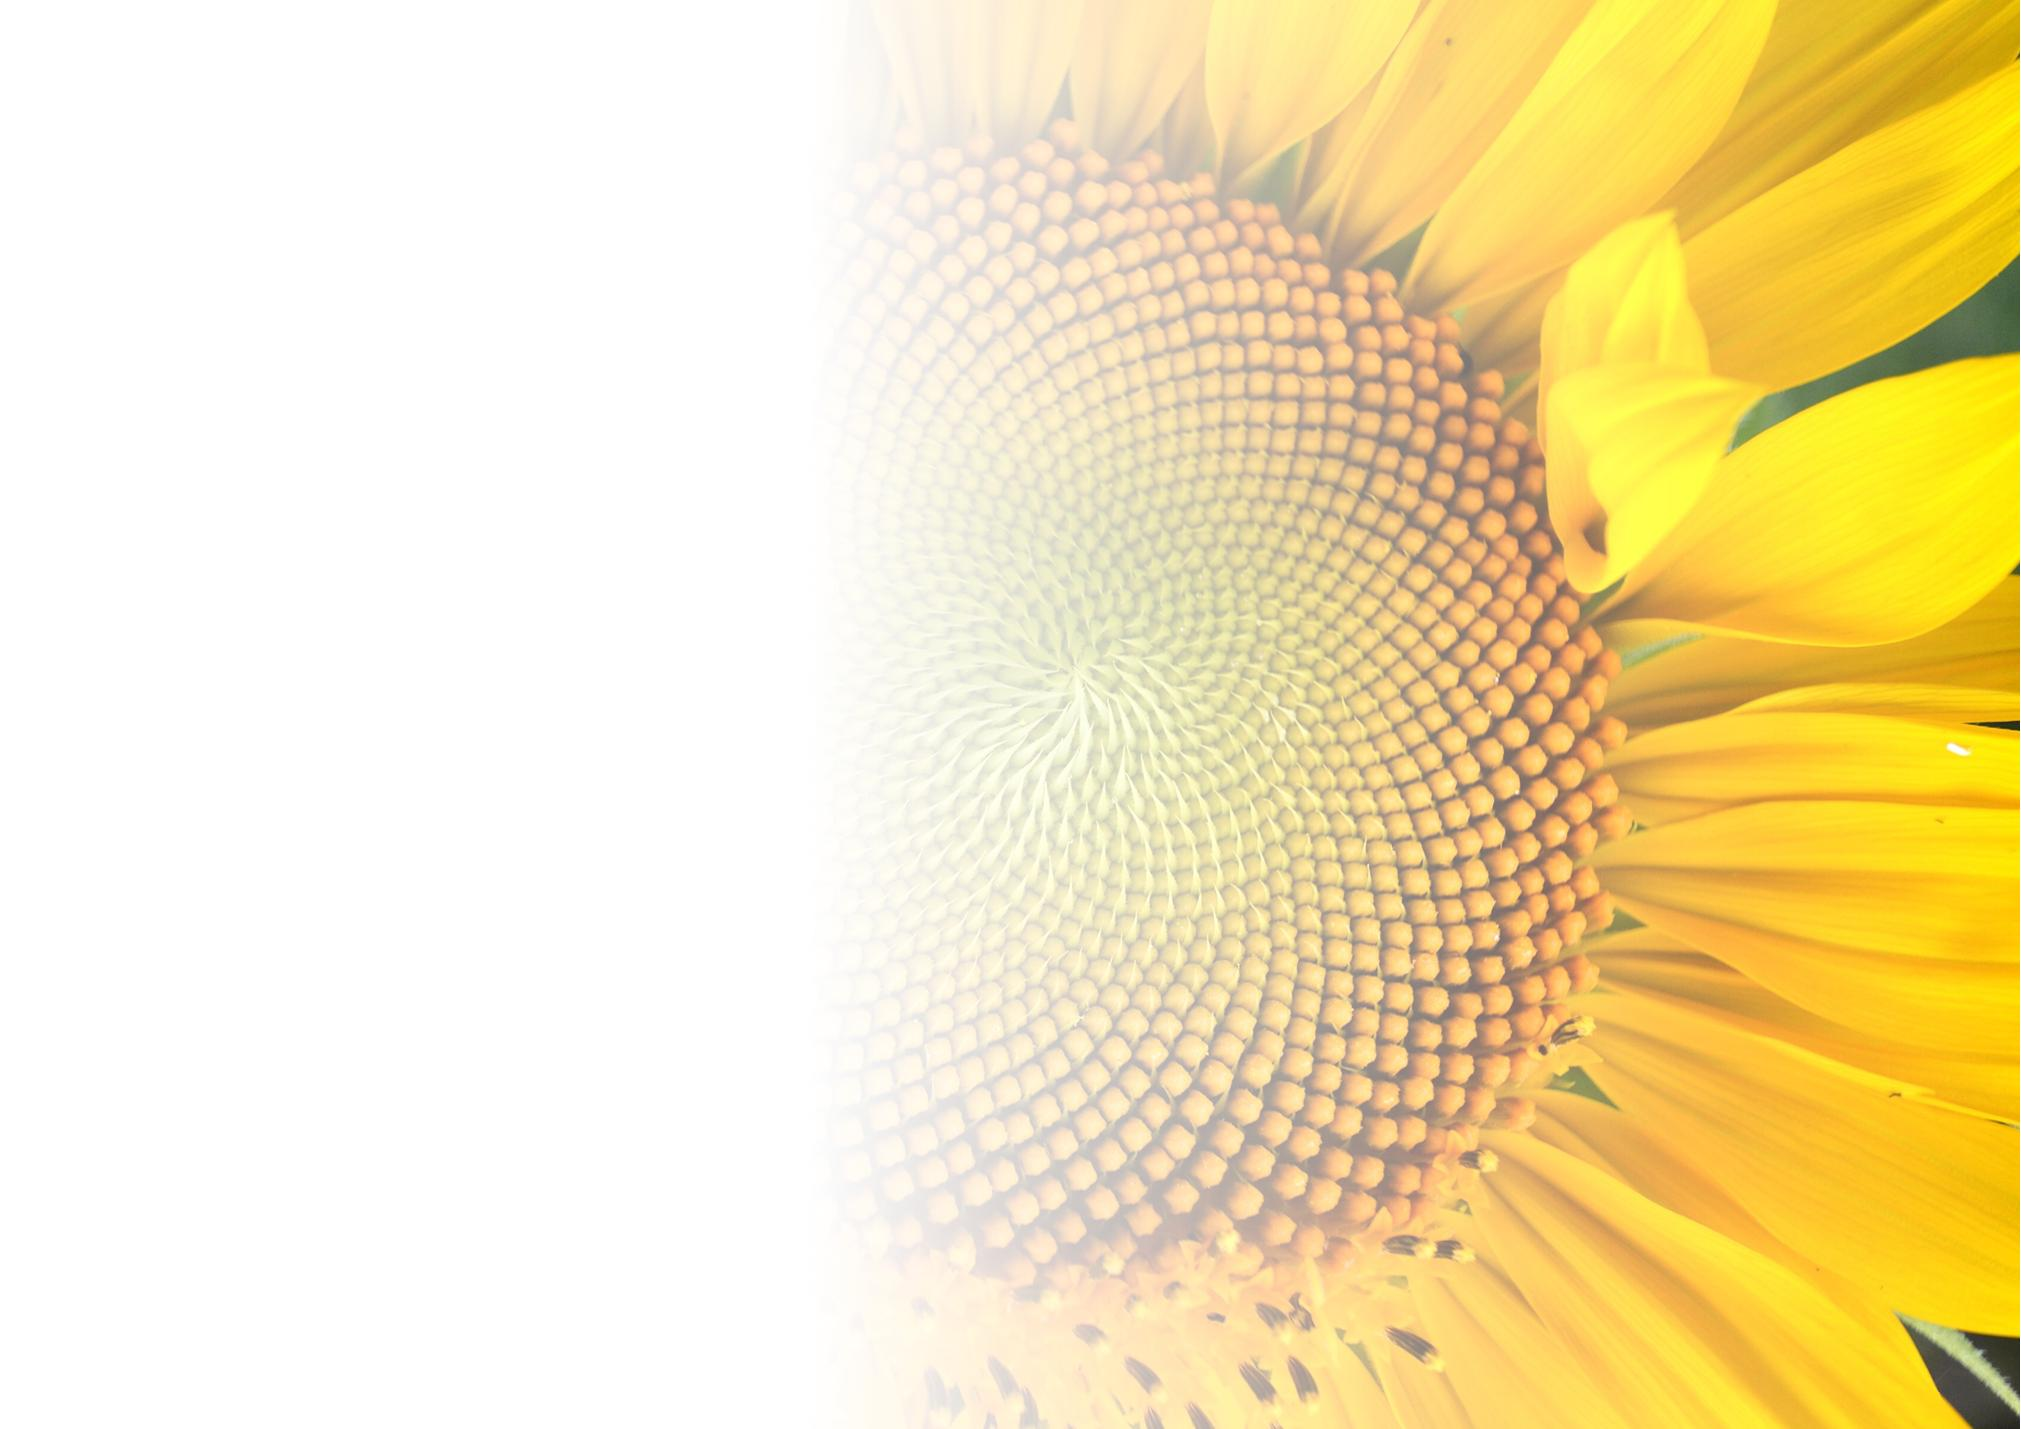
\includegraphics[width=\paperwidth,height=\paperheight]{./Figures/aikoFade.jpg}%
		}%
	}
	\centering
	{\Huge A textbook of }
	\\[3ex]
	{\HUGE\jEmphasisColour	\textsc{Mathematical phyllotaxis}}\\
	\vfill
	{\Huge	\scshape Jonathan Swinton}
	\\\vfill{\jEmphasisColour This is a DRAFT version \jdraftnumber{}}
	\vfill
	{\Large	To appear in Springer \textit{Texts in Applied Mathematics}}
	\\[3ex]
	{\Large \textsc{\jPublicationYear}
		\\}
}
\newpage
\thispagestyle{titlingpage}


\chapter*{Notes to copyeditors}
This is edition \jdraftnumber\  of \textit{A Textbook of Mathematical Phyllotaxis}. This edition is © 2024 by Jonathan Swinton.

A first edition, privately printed in 2023 with the ISBN 978-0-9931789-6-2, is no longer available. 

A small number of images are copyright by others.  The front cover image is taken from the Flickr stream of user \texttt{aiko vanhulsen} under a Creative Commons CC BY 2.0 license. 


\vfill
\begin{tabular}{|c|}
	\hline
	GitHub for document source and Mathematica figure generation
	\\
	\url{https://github.com/js229/MathematicalPhyllotaxis}
	\\
	Branch
	\\ \texttt{\jGithubMathematicalPhyllotaxisRepoBranch}
	\\
	Last commit 
	\\
	\jGithubMathematicalPhyllotaxisRepoTimeStamp
	\\
	SHA \\
 \texttt{\jGithubMathematicalPhyllotaxisRepoSHA} 
	\\ \hline
	Compiled  \\ \today.
	\\\hline
\end{tabular}

\newpage
\listoffigures



\chapter*{Preface}


Over the past hundred years or more there has been a confusing variety of attempts to explain in mathematical language why Fibonacci numbers appear in plant spirals, but most modern accounts have now converged on a framework which might be called a Standard Picture. This book explains that mathematical framework and explores the extent to which it can explain Fibonacci phyllotaxis in the light of modern molecular biology.
 This Standard Picture relies on a biological model of how plants decide where to place individual new  organs over the course of development,
a model which when iterated tend to produce patterns we can model mathematically as lattices. Straight lines in these lattices are \textit{parastichies}, with an associated parastichy number counting how many of the parastichies make up the lattice, and there is a natural way to model what we do when we visually identify spirals as obvious that selects two of these parastihy numbers as the \textit{principal parastichy pair}.  This enables us to classify many model patterns by pairs of integers. Then we change a parameter of the model slowly, corresponding to some slow change -- almost always geometry -- in the underlying developmental process. This gives us a bifurcation tree for principal parastichy pairs as that parameter varies. The culmination of the Standard Picture is that, under quite general assumptions, Fibonacci-like structures form  stable branches of solutions.

It has been my goal in this book to equip readers to critique and participate in the applications of mathematical phyllotaxis.  I aim to give you an understanding of enough of the underlying biology to motivate this Standard Picture, to analyse it mathematically, and to evaluate it scientifically. Actually the main goal was to learn about the subject myself, but in writing the text I have imagined the needs of a recently graduated student of mathematics embarking on research in an interdisciplinary laboratory. (Since I don't fit any of these criteria, I would be particularly grateful for critique from those who do.) This is a textbook in which I have re-shaped and sometimes  re-derived a lot of other people's work into a story I find coherent and worth sharing. I have not felt obliged to provide a source for every statement or idea. Notes to each Chapter situate it in the literature for further reading. 



The first half of the book is an account of the mathematical theory of two-dimensional lattices. While lattice theory in higher dimensions has been an important area of mathematical research, the much simpler results we need in two dimensions are well-established, and I think intuitive. However my account is regrettably dense with Theorems and proofs. This was not my original aspiration, but evolved as I tried to make sense of multiple overlapping concepts, and occasional mathematical untruths, in the phyllotaxis literature.  So there is in places a density of mathematical argument of the pedantic kind I learned to loathe when a graduate student many decades ago. To my surprise, in the end I rather enjoyed writing these parts, but for those whose taste does not run this way they are largely skippable. I have put less technical summary sections at the ends of these chapters.  


The second half of the book connects the mathematical principles of the first half to biological observation by reviewing a range of mathematical models. This part reviews some basic plant embryology and molecular biology and introduces the apical meristem as the site of developmental and positional commitment. I will discuss older ideas, like Hofmeister's hypothesis that primordia are generated as soon as they are beyond a fixed distance from all other primordia, together with the modern molecular understanding of  auxin-based mechanisms of primordia initiation. Then we can begin the applied mathematical work of evaluating how well our lattice models perform, and what they do and don't explain. In particular, we will see the mathematical and biological motivations for generalising lattice models to stacked-coin models. Finally we'll  review some of the outstanding mathematical questions, both pure and applied, and how they can inform the wider and continuing scientific debate on the generation of form in biology.

%Finally, to rephrase the advice buried above: skip all the mathematics you want, especially on a first reading. 






\begin{KeepFromToc}	\tableofcontents\end{KeepFromToc} 
\addtocontents{toc}{\vfill}
\part{Introduction}


\chapter{Motivation and outline}
The Fibonacci series is
\[
0, 1, 1, 2, 3, 5,8, 13, 21, 34, 55, 89, 144, \dots
\] where each number after the second is the sum of the previous two. Phyllotaxis means the arrangement of the organs of plants, like leaves and seeds,  and Fibonacci phyllotaxis is a reference to the appearance of Fibonacci numbers in different kinds of counts of these organs. 
 \jpgfig{BletchleyDaisyCrop}{Thirteen green bracts on the underside of a Bletchley Park daisy \textit{Bellis perennis}, picked in 2019 from the lawn where Joan Clarke taught Alan Turing about phyllotaxis in the summer of 1941.}{0.5}

\section{Joan Clarke's daisy}

%
 For a few months in the summer of 1941, a young British couple were engaged to be married. Both were talented and overworked cryptographers working at Bletchley Park, the wartime codebreaking station, and  
 Joan Clarke and Alan Turing would spend their off-duty hours together, playing chess,  going for bicycle rides and visiting each other's parents. They broke the engagement off after a disastrous wet weekend in Wales, but when in the 1970s Turing's biographer Andrew Hodges interviewed Clarke, what she remembered distinctly about her long summer with her fianc\'e was lying on the lawn in front of Bletchley Park looking at the daisies. Turing and Clarke already knew about and shared an enthusiasm for the appearance of Fibonacci numbers in plants and though both were first-class mathematicians, it was Clarke who had to teach Turing about the botanical classifications of plant structure. So perhaps she  pulled up one of the summer daisies and explained that the distinct green `petals' on the underside of the flower should be called bracts, but either way, when they counted the bracts they will  most likely have found thirteen of them, as I too did in the summer of 2019 (Figure~\ref{fig:BletchleyDaisyCrop}).

\mmafig{Ch1Sunflower91}{
	Seeds packed onto the head of a sunflower. Three separate sets of spirals have been identified. For each set every tenth spiral is marked with a thick line.  To me the most visually obvious spiral set is the red one of which there are 55, curving anticlockwise as they move outwards, the next the set of 34 clockwise blue spirals, but the set of 89 green spirals is also prominent towards the outside and especially in the upper right hand region. This sunflower head was labelled as sample 91 in~\cite{swintonNovelFibonacciNonFibonacci2016}, and is typical of the more ordered arrangements described there.
}{.8}
Clarke went on to be a significant figure in post-war British cryptography, but it is Turing's legacy which is of course now very well known both inside and outside mathematics.
Undergraduates studying mathematical biology encounter his Turing instability as a mechanism for pattern formation, but what is less commonly taught is that one of the unpublished motivations for his published theory was to explain the appearance of Fibonacci numbers. Indeed, at his death he left behind a manuscript scrap, \textit{Outline of the Development of the Daisy}. Turing died tragically before he fully worked out his theory, although thirty years later other mathematicians, not aware of his work, would take more or less the same direction to reach the mathematics which we are now able to outline in this book. 


\section{The sunflower}

As part of the Turing birth centenary celebrations in 2012, the Museum of Science and Industry in Manchester invited members of the public across the globe to grow sunflowers, \textit{Helianthus annuus} and send them, or pictures of them, into the museum, as a citizen science experiment to determine the prevalence of Fibonacci numbers in the spirals of the sunflower head. Figure~\ref{fig:Ch1Sunflower91} shows one such submission, with different spirals visible to the eye, 
and coloured highlighting showing that these spirals can be organised in families with either 34, 55, or 89 members, at least around the rim of the sunflower, and that the subjective question of which family is most prominent has a different answer at different places in the sunflower.  This is a typical seedhead recorded in the experiment, in which a family of spirals with a Fibonacci count was seen in 74\% of the sample, so that deviations from Fibonacci structure were a common minority.

  The mature seedhead provides useful evidence about the relative position on the plant that the cell lineages leading to each seed occupied when they were making the decision to commit to develop into a seed at all. In particular the centre of the seedhead is newest in the sense that as we move into the centre the seeds are the ones which have arisen from the most recent decisions to commit and the pattern on the outside of the sunflower is laid down before that towards the centre.  In this sample there is a suggestion of a change from ${55,89}$ to ${34,55}$ in the pairs of most prominent parastichy counts over developmental time: this is called a falling phyllotaxis. 

Sunflower parastichy counts like 55 and 89, and occasionally 144 and very occasionally 233, are the largest Fibonacci numbers which can reliably be observed in any plant forms. A common Just So explanation for these observations is that they provide some form of selection advantage for the plant in allowing an `optimal' packing of the seedhead. But it is important to recognise that these large numbers are \textit{not} seen in population subject to natural selection, but in the giant forms of the sunflower, with seedheads 30cm or more across, which have been under intensive breeding pressure by humans over the ten thousand years or so that we have been relying on the sunflower as a food source. 
The evidence of the archaeological record is that both
 the sunflower seed, and the capitulum in which it sits, have grown larger over the development of agriculture, and that this has happened more than once in different human cultures~\cite{lentzSunflowerHelianthusAnnuus2008,burkeGeneticAnalysisSunflower2002}. It is likely that any selection pressure was for increased overall seed-mass, rather than any direct human desire for `optimal packing'. Nevertheless, more modest Fibonacci numbers do recur in other, less genetically modified species. 
\clearpage
\section{Fibonacci structure across the plant kingdom}
 \jpgfig{ChurchEuphorbia}{Four sucessive sections of the stem of a \textit{Euphorbia Wulfenii} in the Oxford Botanic Garden,
 	photographed by AH Church in 1904. From~\cite{churchRelationPhyllotaxisMechanical1904}.}{0.9}
 Daisies and sunflowers are close relatives within what modern taxonomy calls the \textit{Asteracaea} family,  and an older name for this family, the \textit{Compositae}, reflects the common structure of most of them, with many individual flowers packed together on a flat composite seedhead or capitulum. Other members of the family, such as the dahlia, can also exhibit pairs of Fibonacci counts.
However Fibonacci phyllotaxis is not at all a feature unique to this family.

Among flowering plants, Fibonacci patterns are also relatively common in the kinds of cacti sold as houseplants in the UK: they can sometimes be seen in, for example the prickly pear. Spurges (\textit{Euphorbiaceae}) are one genus of shrubs which are interesting in demonstrating rising phyllotaxis in a fairly clear way. One of the earliest systematic British studies of Fibonacci patterns was carried out by the Oxford botanist Arthur Harry Church, and self-published by him from 1904.  Figure~\ref{fig:ChurchEuphorbia} shows the stem of a spurge growing outside his office in the Oxford Botanic Garden.
%
Church has removed all of the former leaves, and in effect numbered each of their positions rising up the stem. Thus when he writes a 3 on the first specimen, he is implying that there are two other branch positions, which we can't see behind the stem. 
The lines drawn by Church in Figure~\ref{fig:ChurchEuphorbia}  are meant to suggest that the branch positions are organised in spirals making up families with, in one case, 13 and 21 members.  Church's book, though dated in places, remains the most valuable compendium of Fibonacci (and non-Fibonacci) structure in phyllotactic counts and is the basis for much of this chapter. For eample he also records that pairs of Fibonacci counts like 5 and 8 can also be seen in the leaf structure of arums (\textit{Arum}), teasels (\textit{Dipsacus}), and crassulas (\textit{Crassulacae}).
 \\\mbox{}
 \clearpage
 \section{The pineapple}
\mmafig{Txb0014LinfordPineapple}{Top: (a) whole pineapple and (b) flattened pineapple skin from~\cite{linfordFruitQualityStudies1933}; the black lines are natural markings on the scales. Bottom: as (b), but with the centre of each scale numbered in order of height in the photograph, and physically adjacent scales joined by lines.}{1.0}
A convenient example of Fibonacci patterning is often available to the supermarket consumer on the form of the pineapple.
\begin{exercise}
	\label{ex:doit}
	Show this.  It is \emph{not enough} to believe that you can find them if you look: you have to look. In the absence of a local grocer, consult Figure~\ref{fig:Txb0014LinfordPineapple}.
\end{exercise}
\begin{solution}
	The grocery proof is left as an exercise to the reader. If using the Linford pineapple, there are clearly 8 spirals going up and to the right; depending on how the scales as the edges were originally joined there are either 12 or 13 spirals up and to the left. 
\end{solution} 
Despite the easily visible presence of Fibonacci spirals in pineapples, Church's systematic 1904 survey of phyllotaxis includes no pineapples or any other representative of their family, the bromeliads. This may have been because at the time whole pineapples were very rarely grown in Europe except as a luxury item, and most pineapple consumed was transferred to Western consumers as a chopped and tinned item from colonial plantations. Indeed, it was not until 1933 that the observation of Fibonacci counts in pineapples made it into the scientific literature, when Linford, working on a commercial plantation, reported the occurrence of Fibonacci counts in a discussion of how to efficiently count the number of eyes~\cite{linfordFruitQualityStudies1933}. The advent of whole fruit transport in the 1950s, enabled  mathematical popularisation to mention the pineapple, notably in the work of Hal Coxeter, and with a suitable meaning for the word `natural',  the pineapple has come to rival the sunflower as an emblem of `mathematics in the natural world'.

 \clearpage
\section{The fir cone}

Fibonacci structure is not restricted to the flowering plants and can also be found in the conifers. 
Figure~\ref{fig:Fierz20151aCrop} shows a fir cone, one of six thousand collected from a black pine tree on the slopes above Lake Zurich in a remarkable experiment by Dr Veronika Fierz. As in the Museum of Science and Industry experiment, the main scientific motivation was to explore deviations from strict Fibonacci structure, but as with sunflowers the data also shows how prevalent Fibonacci structure was: all but a few hundred had eight spirals of the seed-protecting scales in one direction and thirteen in the other. 
%
\jpgfig{Fierz20151aCrop}{One of over 6000 pine cones of a single \textit{Pinus negra} studied by Fierz, of which 97\% had, like this specimen, eight spirals visible in in direction and thirteen in the other. The cone was attached to the tree through the central region, with the growing tip furthest away from the camera, so that the scales are numbered by youth, with scale 0 developing after the others. The thirteen spirals are outlined directly; that there \textit{are} eight in the other direction can be confirmed by picking out eg the sequence $2,10,18,26,34,\ldots$ and seeing we can do this eight times.  From~\cite{fierzAberrantPhyllotacticPatterns2015}. \copyright CC-BY 3.0 Fierz, 2015.
	}{1}
\clearpage
\begin{exercise}
	\label{ex:doitagain}
	Use Braun's 1831 drawings (Figure~\ref{fig:Braun1831}) of pine cones with the scales numbered to count the spirals they display.
\end{exercise}
\begin{solution}
Based on the consistent jumps between adjacent numbered scales (eg in Fig 1, from 22 to 26 to 40 to 34 is evidence of four separate spirals), I would say these cones display evidence of 4 and 7 spirals (Fig 1); 7 and 11 (Fig 2); 7 and 10 (Fig 4a). Based on the scale numbering alone, I can't assign an unambiguous spiral count  for Fig 3. 
\end{solution}

Fibonacci counts, typically but not always 3s, 5s and 8s, can be found in the fruit cones of other conifers, including spruces (\textit{Picea}), larches (\textit{Larix}),  cypresses (\textit{Cupressus}) \cite{fierzAberrantPhyllotacticPatterns2015} and the monkey-puzzle tree (\textit{Araucaria}) \cite{churchRelationPhyllotaxisMechanical1904}. 

\clearpage
\subsection{Monocots and dicots}
Much importance will attach in this book to considering the development of complexity from an initial simple pattern, so it is natural to pay attention to the initial pattern formed when the first embryonic leaf structures emerge from the seed. Most flowering plants are dicotyledons, meaning that these proto-leaves emerge as a pair, but a few are monocotyledons, in which 
only a single proto-leaf emerges. The pineapple family of bromeliads, for example are monocots. Although the distinction between monocots and dicots was once a major taxonomic classification, it is now believed that the ancestor of all flowering plants was a dicotyledon, and this symmetry was broken several different times in multiple cases of convergent evolution~\cite{ingrouillePlantsDiversityEvolution2006}. 
\jpgfig{Braun1831}{Spruce  \textit{Picea} cones from from Plate XXVII of~\cite{braunVergleichendeUntersuchungUber1831}; Fig 4(b) is the back view of Fig 4(a).}{1.0}


\section{Stem primordia}
The preceding examples of large Fibonacci numbers, detectable on a a macroscopic scale in the mature plant form, are more or less the only ones documented in the scientific literature, and so come from a very small fraction indeed of the `endless forms most beautiful' that Darwin spied in biological organisms, but it would be wrong to dismiss these cases as therefore uninformative on the processes generating plant form in general. Similar structures, albeit associated with much lower Fibonacci numbers, are very common indeed in the early embryonic forms of very many plant stems. 
\newpage

 \section{Summary}
 There are many accessible example of Fibonacci phyllotaxis: perhaps the most robustly repeatable observation for city-dwellers is to buy a pineapple. However for most species, including the pineapple,  large-scale scientific data is surprisingly sparse on the exact prevalence of different kinds of patterns, and especially on the ways in which patterns fail to be Fibonacci. An argument of this book is that it is when patterns fail to be Fibonacci that they are most informative for model testing, and we will return to this in the second half of the book. 
% \mmafig{Ch1Phylogeny}{A simplified phylogenetic tree of the vascular plants showing six of the species listed by Church~\cite{churchRelationPhyllotaxisMechanical1904} as displaying some kind of Fibonacci-related patterning. The flowering plants are thought to have diverged from the conifers about 300 million years ago (MYa)}{1}
\jEndChapter


\chapter{Fibonacci and the golden ratio}

\label{CH:0}
\label{ch:0}
\section{Fibonacci sequences}

The Fibonacci sequence $F_n$ has as its first two members  $F_0=0$, $F_1=1$ and every subsequent member is the sum of the previous two:  $F_{n+2}=F_{n+1}+F_{n}$. 
Although there is a substantial literature on Fibonacci and related sequences~\cite{vajdaFibonacciLucasNumbers2008} we really only need this simple sum property for the Standard Picture. 
A related sequence is the Lucas sequence  ($1,3,4,7,11,\ldots$) with the same rule but different initial conditions, both Fibonacci and Lucas numbers are special cases of the generalised Fibonacci numbers with starting pair $F^k_1=1$, $F^k_2=k$. We will also encounter the sequence created by doubling each Fibonacci term, for which terminology varies but I'll call a double-Fibonacci sequence. 
%
\begin{table}[ht]
	\begin{center}
		\begin{tabular}{ll}
			\hline
			Fibonacci  &  $1,1,2,3,5,8,13,21,34,55,89,144,\ldots$ 
			\\
			Double Fibonacci & $2,2,4,6,10,16,26,42,68,110,\ldots$
			\\
			Lucas ($F3$)&      $ 1,3,4,7,11,18,29,47,76,123,199\ldots$
			\\
			$F^4$  & $1,4,5,9,14,23,37,60,97,157\ldots$
			\\
			$F^5$ & $1,5,6,11,17,28,45,73,118,191\ldots$
			\\
			\ldots &
			\\
			$F^8$ & $1,8,9,17,26,43,69,112,181\ldots$
			\\
			\hline
		\end{tabular}
		\caption{Various sequences with Fibonacci structure}
		\label{tab:sequences}
	\end{center}
\end{table}
%

We might note that from Table~\ref{tab:sequences} that the Fibonacci, double Fibonacci and Lucas sequences together include all  of the first eleven integers except 9, so there is little remarkable about the observation that a particular system exhibits a structure including a low member of one of the sequences~\cite{cookeFibonacciNumbersReveal2006}. Finding pairs of adjacent members of the same series, or examples of numbers greater than ten, would be more significant.

\subsection{The golden ratio}
Starting the sequence with $F_0=0$, $F_1=1$, the general Fibonacci term is 
\begin{eqnarray}
F_n &=& \frac{\tau^n - (1-\tau)^n}{\sqrt{5}}
\end{eqnarray}
where $\tau$ is the golden ratio 
satisfying
\begin{eqnarray}
\tau^2 &=& \tau+1
\\
\tau &=& \frac{1+\sqrt{5}}{2} \approx 1.618
\\
&=& \lim_{n\rightarrow\infty} \frac{F_{n+1}}{F_n} 
\end{eqnarray}
Any sequence obeying the Fibonacci rule has $\tau$  as the limit of the ratio of its terms.

\subsection{The golden angle}
The golden angle is
\[
\Phi = \frac{2\pi}{\tau^2}  \approx 137^\circ
\]
so
\[
\frac{\Phi}{2 \pi} \approx \frac{F_{n}}{F_{n+2}}
\]
As we'll see, the angular rotation between successive leaf structures is often very close to this angle for Fibonacci (but not, for example, Lucas) phyllotaxis.




\section{Co-prime integers}

\label{sec:coprime}
Two integers $(m,n)$ are co-prime iff\jNote{The word `iff' is not a typo. It means if and only if, and is also a shibboleth.
	If it is bewildering to you that `iff' means logical equivalence and not just implication then you have not been inducted into the kind of mathematical exposition, roughly first-year undergraduate, we use until around section~\ref{sec:ClassifyingSummary}, so you will want to skip to there. On the other hand you can read all of the rest of the book without knowing what a shibboleth is.} their greatest common divisor is equal to 1, so that for example 4 and 11 are co-prime. We need to be explicit about some edge cases, by noticing that every integer is a divisor of $0$, but the only divisors of $1$ are $1$ and $-1$. Specifically we recognise both of the pairs $(0,1)$ and $(1,n)$ as co-prime, and note that $1$ is co-prime to itself, but $0$ is not, and $(0,n)$ is not co-prime for $n>1$.%
%\footnote{We don't require the integers to be non-negative for this co-primality to make sense, but we avoid situations where this matters.}

\chapter{Co-primality, continued fractions, and M\"obius maps}
It would be wise to skip, or read very glancingly, this chapter on a first reading. 
The material on co-prime integers and B\'ezout relations are only needed for those who want to closely follow the proofs of Chapter~\ref{ch:cylinder}. M\"obius maps are the main language of  the renormalisation approach to the van Iterson diagram discussed at the end of Chapter~\ref{ch:classifying}, but are not at all essential to understand the biological implications of the mathematics.  The details of the matrix form of the Euclidean algorithm may only matter to those curious about the relationships between Fibonacci phyllotaxis and Escher prints.


\section{B\'ezout relations}
The previous chapter defined co-primality for a pair of integers. An equivalent condition is the existence of a  B\'ezout relation: the integer pair $(u,v)$ satisfies the B\'ezout relation for the non-negative integer pair $(m,n)$ iff
\begin{align}
	|n  u-mv| = 1.
\end{align}
So $(3,4)$ are a B\'ezout pair for $(8,11)$. 
If $u$ and $v$ exist then they are a certificate of co-primality: we will see below that $(m,n)$ can satisfy  $ n  u - m v= k$ iff $|k|$ is the greatest common factor of $m$ and $n$. They are not unique because if $(u,v)$ satisfies the B\'ezout relation then so does $(u+km,v+kn)$ for any integer $k$: $(11,15)$ is also a B\'ezout pair for $(8,11)$. We can introduce a range condition by picking a particular $k$ which can be used to enforce $0\leq v< n$, but there is still a further ambiguity because if
$n u- m v  =+1$ provides one solution, then $n(m-u)-m(n-v)=-1$ provides another: because $11\times3-4\times8 =+1$ we can find $11\times 1-4\times 3=-1$. 

\section{The winding-number pair}
\label{sec:wnp}
There are different ways to cope with the non-uniqueness of  B\'ezout pairs.
Here we pick out a particular pair, the \textit{winding-number pair}. 
For co-prime integers  $(m,n)$, the winding-number pair is the unique pair  $(u,v)$ which satisfies the B\'ezout relation $|n  u-mv| = 1$ and also
\begin{align}
	0\leq \frac{u+v}{m+n}\leq \frac{1}{2}. \label{eq:wnpFarey}
\end{align}
There are a handful of special cases: in this book the winding-number pair for  $(0,1)$ is by definition $(1,0)$, for $(1,0)$ is $(0,1)$, and for $(1,1)$ is $(1,0)$. 
As we will see below, half of the time the winding-number pair will yield $nu-mv=+1$ and half the time $n u-m v=-1$. We could alternatively have found a unique pair by insisting on a particular choice of sign $nu-mv=+1$, but in this way there is a clear connection to the signs of the $\Delta$s that will pepper Chapter~\ref{ch:cylinder}. Chapter~\ref{ch:cylinder} will also reveal the reason for the name `winding-number pair'. 


\begin{jExercise}{ex:wnp}
	Compute the winding-number pair for $(m,n)$ for co-prime $m,n$ less than 10. 
\end{jExercise}
\begin{jAnswer}{ex:wnp}
	Some winding-number pairs are given in Table~\ref{tab:wnp2}.
	\begin{table}
	\begin{equation*}
		\begin{array}{lllll}
			\hline
			\\
			\jFarey{u}{m}{v}{n}
			&\jFarey{0}{1}{1}{0}&   &  &   \\[2ex]
			\jFarey{ 1}{0}{0}{1} &  \jFarey{1}{1}{0}{1}  &  \jFarey{1}{2}{0}{1}  & \jFarey{1}{3}{0}{1}& \jFarey{1}{4}{0}{1} \\[2ex]
			&  \jFarey{0}{1}{1}{2}&  & \jFarey{1}{3}{1}{2} &  \\
			&  \jFarey{0}{1}{1}{3} & \jFarey{1}{2}{1}{3} &  & \jFarey{1}{4}{1}{3} \\[2ex]
			&  \jFarey{0}{1}{1}{4} &  & \jFarey{1}{3}{1}{4} & \\[2ex]
			&  \jFarey{0}{1}{1}{5} &\jFarey{1}{2}{2}{5} & \jFarey{1}{3}{2}{5} &\jFarey{1}{4}{1}{5} \\[2ex]
			&  \jFarey{0}{1}{1}{6} &  &  &  \\
			&  \jFarey{0}{1}{1}{7} &\jFarey{1}{2}{3}{7}& \jFarey{1}{3}{2}{7} & \jFarey{1}{4}{2}{7}  \\[2ex]
			&  \jFarey{0}{1}{1}{8} &  & \jFarey{1}{3}{3}{8} &  \\[2ex]
			&  \jFarey{0}{1}{1}{9} & \jFarey{1}{2}{4}{9} &  & \jFarey{1}{4}{2}{9}  \\[2ex]
			\hline
		\end{array}
	\end{equation*}
		\caption{Winding number pairs given as Farey intervals $[u/m,v/n]$. For $m$ and $n$ positive and distinct these are all contained in $[0,\jhalf]$ but the natural order of the endpoints varies with the sign of $mv-nu=\pm 1$.}
		\label{tab:wnp2}
	\end{table}
\end{jAnswer}



For the small integers in plant spiral counts it is perfectly feasible to compute highest common factors and winding-number pairs by exhaustive search. But nevertheless the rest of this Chapter shows how an algorithmic approach sheds a light on the structure of co-prime pairs and their winding-numbers in a way that has been helpful in the past to mathematicians puzzling over Fibonacci structure. 


\section{Euclid's algorithm}
\label{sec:euclid}
Euclid's algorithm finds the highest common factor of two positive integers by repeatedly subtracting the smaller as many times as we can from the larger to find a new, smaller pair of integers,  stopping when one of them is zero. It is  simple to implement, and tracking the variables in the intermediate steps of the algorithm will allow us to understand connections with continued fractions and structure of the van Iterson diagram of Chapter~\ref{ch:cylinder}.
For example, consider calculating the highest common factor of $4$ and $11$:
\begin{align}
	11 - {\jHeadingColour 2}\times 4 & = 3 
	\\
	4 - {\jHeadingColour 1}\times 3 & = 1\label{eq:411}
	\\
	3 - {\jHeadingColour 3}\times 1 & = 0 
\end{align}
%
This works by successively answering the question of how many times 4 goes into 11 (ie ${\jHeadingColour 2}$), 3 into 4  (${\jHeadingColour 1}$), and 1 into 3 (${\jHeadingColour 1}$) and generates 
a particular sequence of what we will call  $\jqi={\jHeadingColour 2, 1, 3}$ which shows the co-primality of 4 and 11. Because of the central role of the $\jqi$ they are coloured in red in what follows. It is possible to use this decomposition to compute the winding-number pair, which we can see if we rewrite the algorithm in more formally. 
Given integers $n\geq m>0$  we set $r_{-1}=n$, $r_0=m$ and $i=0$:
\begin{enumerate}
	\item Set an integer $\jqi=\lfloor r_{i-1}/r_i \rfloor $, to non-negatively minimise $r_{i-1}-q r_{i}$ 
	\item  Set  $r_{i+1}=r_{i-1}-\jqi r_{i}$. 
	\item If $r_{i+1}=0$, set $N=i$ and terminate.
	\item Otherwise increment $i$, and repeat.
\end{enumerate}
\begin{theorem}
	Euclid's algorithm terminates with the greatest common factor $GCF(m,n)$:
	\begin{eqnarray}
		r_N =  
		GCF(m,n) 
	\end{eqnarray}
\end{theorem}
\begin{proof}
	The $r_i$ are a strictly decreasing sequence of positive integers and so the algorithm always terminates. Suppose the $GCF$ is $k$. Now $k$ divides $r_0$, $k|r_0$, and the $i$-th step of the iteration preserves the fact that  $k|r_i$,  and so in particular $k|r_N$. Now $r_N|r_{N-1}$ and the iteration step also shows that if $r_N|r_i$ and $r_N|r_{i-1}$ then $r_N|r_{i-2}$, and so following the $r_i$s in reverse order we see $r_N$ divides all of them and divides both $m$ and $n$.  So $r_N$ is a common divisor and so $r_N\leq k$ but since $k|r_N$, $r_N=k$. 
\end{proof}

\subsection{Matrix form of the Euclidean algorithm}
\mmafig{Txb0031EuclideanTree}{Computing the highest common factor of 4 and 11 by successive matrix reductions upwards to the identity matrix. Conversely, the extended tree downwards from the identity matrix, branching by an $E$ or an $ES$ matrix-multiplication at each node after the second, will contain every pair of co-prime integers, in the first column of each matrix, with the corresponding winding-number pair in the second column. 
The $\jqi$s of the Euclidean reduction emerge as the number of $E$s between each $S$.}{1}
%
We can solve the B\'ezout relation by putting  Euclid's algorithm in matrix form. For example
the first reduction of~\eqref{eq:411} is
\begin{align*}
\begin{pmatrix} 11 \\ 4 \end{pmatrix}  &= \begin{pmatrix} 1 & \jqn{2} \\ 0 & 1\end{pmatrix} \begin{pmatrix} 3 \\ 4\end{pmatrix} 
\\
&
= \begin{pmatrix} 1 &1 \\ 0 & 1\end{pmatrix}^{\jqn{2}}  \begin{pmatrix} 0 & 1  \\ 1 & 0  \end{pmatrix} \begin{pmatrix} 4 \\ 3 \end{pmatrix}
\\
&=
E^{\jqn{2}} S \begin{pmatrix} 4 \\ 3 \end{pmatrix}
\end{align*}
where we have defined matrices  $E$ corresponding to a  `Euclidean' reductions and $S$ corresponding to `swap' of the integer pair. Matrix algebra shows $E^\jq$ has a $q$ in the upper-right corner:
\begin{align*}
	E^{\jq} &=  \begin{pmatrix} 1 & \jq \\ 0 & 1\end{pmatrix}
	;
	S =  \begin{pmatrix} 0 & 1  \\ 1 & 0  \end{pmatrix}
	;
	E^{\jq} \cdot S = \begin{pmatrix}\jq & 1  \\ 1 & 0  \end{pmatrix}
\end{align*}
Moreover  $\det E=1$ and $\det S=-1$ and so the matrix of any product of $E$s and $S$s has determinant of modulus 1. 

After we learn the $\jq$ sequence through the Euclidean algorithm we can write the result in matrix form as 
\begin{align*}
	\begin{pmatrix} 11 \\ 4 \end{pmatrix}  &= 
	(E^{\jqn{2}} S )\cdot( E^{\jqn{1}} S ) \cdot (E^{\jqn{3}} S)  \begin{pmatrix} 1 \\ 0 \end{pmatrix}.
\end{align*}
If we apply the same series of transformations to the column vector $(0,1)$ we will obtain a column vector of the form $(v,u)$  so that
\begin{align}
		M_{\jqn{2}\jqn{1}\jqn{3}}= \begin{pmatrix} 11 & v \\ 4 & u \end{pmatrix}   &= 
	(E^{\jqn{2}} S )\cdot( E^{\jqn{1}} S ) \cdot (E^{\jqn{3}} S) 
	 \begin{pmatrix} 1&0  \\ 0&1 \end{pmatrix} 
	 \label{eq:M213}.
\end{align}
This shows that  $u$ and $v$ which satisfy $|4 v-11 u|=1$ and give us a B\'ezout relation, and since $\det E=1$ but $\det S=-1$, the sign of the determinant of $M$ is determined by how many $S$ matrices appear in the product. It also provides a way to calculate $u$ and $v$:
\begin{align*}
	M_{\jqn{2}\jqn{1}\jqn{3}}&=
	 \begin{pmatrix} 2 & 1 \\ 1 & 0 \end{pmatrix}\cdot
 \begin{pmatrix} 1 & 1 \\ 1 & 0 \end{pmatrix}\cdot
	  \begin{pmatrix} 3 & 1 \\ 1 & 0 \end{pmatrix}
	 	 \\
	 &= \begin{pmatrix} 11 & 3 \\ 4 & 1 \end{pmatrix}
% \label{eq:M213value}.
\end{align*}
For a general $m$ and $n$, using the $\jqi$ values from the Euclidean algorithm gives us 
\begin{align}
	M_{\jqn{q_1}\jqn{q_2}\cdots\jqn{q_N}}=\begin{pmatrix} n & v \\ m & u \end{pmatrix}   &= 
	(E^{\jqn{q_1}} S )\cdot( E^{\jqn{q_2}} S ) \cdots  (E^{\jqn{q_N}} S)  \begin{pmatrix} 1&0  \\ 0&1 \end{pmatrix}.
	\label{eq:EuclideanMatrixq}
\end{align}
%Dropping the $\jq$s now, we will 
%\begin{align}
%	M_{nm} &=\begin{pmatrix} n & v \\ m & u \end{pmatrix} 
%	\\
%	\Delta_{nm} &= \det 	M_{nm}
%	\\
%	|\Delta_{nm}| &= 1
% 	\label{eq:EuclideanMatrix}
%\end{align}

Because every pair of co-prime integers has a unique $\jqi$ sequence, every pair such pair will appear exactly once in the first column of a matrix in the tree generated by continuing Figure~\ref{fig:Txb0031EuclideanTree} downwards.
The second column is the corresponding B\'ezout pair. The same algorithm also works when $m$ and $n$ are not co-prime:
\begin{jExercise}{ex:showk}
	Show that if $m$ and $n$ have highest common factor $k$ then $u,v$ found in this way give $|nu-mv|=k$.
\end{jExercise}
\begin{jAnswer}{ex:showk}
	Multiply~\eqref{eq:EuclideanMatrixq} by $k$
\end{jAnswer}
As we will see in the next section, this B\'ezout pair is in fact the winding-number pair.

\begin{jExercise}{ex:f1}
	Show that for $j>1$ the  $\jqi$ for the Fibonacci pair $F_{j+1}$ and $F_j$ are a sequence of 1s of length $j$ and 
	the pair have a B\'ezout pair, but not a winding-number pair,  $F_j$ and $F_{j-1}$.
\end{jExercise}
\begin{jAnswer}{ex:f1}
		It is easy to show by induction that 
\begin{align}
	\begin{pmatrix} 
		F_{j+1} & F_{j} 
		\\
		F _j & F_{j-1}
	\end{pmatrix} &= 	(E^\jqn{1} S)^{j}.
	\label{eq:FibonacciMatrixB}
\end{align}
So the  $\jqi$'s are all \jqn{1} and the determinant shows that $(F_{j},F_{j-1})$ is a B\'ezout pair. It is not a winding-number pair because $F_{j-1}/F_j>\jhalf$. Note these are not the matrices that appear in Figure~\ref{fig:Txb0031EuclideanTree}.
\end{jAnswer}

Any integer can be represented as a sum of two multiples of basis integers, and looking at the Euclidean algorithm from a broader perspective, it can  be seen as a series of changes of these bases.  The individual $E^{\jqi}$ matrices correspond to  M\"obius transforms that change base at each step, the product matrix is the change of basis between $m,n$ and $k,1$, and the $ |mv - nu|=k$ relationship tells us about how areas are scaled in the different bases. 

\section{Farey trees and winding-number pairs}

Thanks to a careful choice of stopping rule for the algorithm, or equivalently because of how we pruned the tree of Figure~\ref{fig:Txb0031EuclideanTree} not to bifurcate from the first two nodes, the $(u,v)$ which emerge from the Euclidean algorithm are not just a pair satisfying the B\'ezout relation but they are exactly the winding-number pair.
%
Each matrix in the tree of Figure~\ref{fig:Txb0031EuclideanTree} is of the form
\begin{align*}
	\begin{pmatrix} 
		n & v
		\\
		m & u
	\end{pmatrix}
\end{align*}
with $nu-mv=\Delta$ and $|\Delta|=1$. For each matrix below the root, we can form two rationals $u/m$ and $v/n$; for  $\Delta=1$, $u/m>v/n$ while for $\Delta=-1$, $u/m<v/n$ but in either case they form the endpoints of a real interval we will call the Farey interval for the matrix. 
The Farey interval of the integers $m, n, u, v$ is $[u/m,v/n]$ although the endpoints may not be in order. 
The Farey sum of these two rational endpoints, or the Farey mediant of the matrix, is $(u+v)/(m+n)$ which is always contained in the Farey interval.
\begin{jExercise}{ex:farey}
	Show this.
\end{jExercise}
\begin{jAnswer}{ex:farey}
	Compute the difference between the Farey sum and the endpoints: the signs of these and the difference between the endpoints are all controlled by the sign of~$\Delta$. 
\end{jAnswer}

Farey intervals for the first few matrices in the tree are shown in Figure~\ref{fig:Txb0032FareyIntervals}.%
\mmafig{Txb0032FareyIntervals}{Farey intervals $[u/m,v/n]$ for matrices $\begin{pmatrix}
		n & v\\ u & m
\end{pmatrix}
$ coloured blue if the determinant of the matrix is $+1$ and left white it is $-1$.
}{1}%
%
If a matrix has a Farey interval of  $[u/m,v/n]$, then multiplication by $E$ gives a new matrix with a Farey interval of $[u/m,(u+m)/(v+n)]$ and multiplication by $ES$ gives one of  $[v/n,(u+m)/(v+n)]$: the interval splits at the Farey sum at each bifurcation. Since the matrix one down from the root has a Farey interval of $[0,\jhalf]$, every matrix below that has its Farey interval within this range, which means that  B\'ezout pair in the second column of each matrix is in fact a winding-number pair.

 Examining the tree also justifies our claim that $m v-nu$ is plus or minus one equally often in the tree (save for the first two nodes), since its sign changes each time there is a multiplication by $ES$ rather than $S$.


\subsection{Fibonacci pairs}
\label{sec:euclidean}
The Fibonacci matrices in Figure~\ref{fig:Txb0031EuclideanTree} are found by consistently choosing the $ES$ branch for each bifurcation from the second node so that, for example
\begin{align*}
	\begin{pmatrix} 
	13 & 5 
		\\
		8 & 3
	\end{pmatrix} &= 	(E S)^{{4}} \cdot E^2 S ;
\end{align*}
and recalling that $F_{7}=13$, this generalises easily to
\begin{align}
	\begin{pmatrix} 
		F_{j+1} & F_{j-1} 
		\\
		F _j & F_{j-2}
	\end{pmatrix} &= 	(E S)^{{j-4}} \cdot E^2 S.
\label{eq:FibonacciMatrix}
\end{align}
%
\begin{jExercise}{ex:fpairs}
	Prove this.
\end{jExercise}
%
\begin{jAnswer}{ex:fpairs} 
\begin{align}
E S \begin{pmatrix} 	F_{j+1} & F_{j-1} 	\\	F _j & F_{j-2}\end{pmatrix}
  &= 	\begin{pmatrix} 1 & 1\\1 & 0 \end{pmatrix}
\begin{pmatrix} F_{j+1} & F_{j-1} \\F _j & F_{j-2}\end{pmatrix}
&= 
\begin{pmatrix} 	F_{j+2} & F_{j+1} 	\\	F _{j+2} & F_{j-1}
\end{pmatrix}
\end{align}
\end{jAnswer}
%
Together with the previous section this shows that the winding-numbers for a pair of adjacent Fibonacci numbers are the two previous Fibonacci numbers.
Moreover we can calculate the associated Farey intervals for use in Chapter~\ref{ch:cylinder}.


\begin{jExercise}{ex:fareyFpair}
	Show  the Farey interval for the Fibonacci pair $(m,n)= (F_j,F_{j+1})$ contains $1/\tau^2=1/(1+\tau)$ but that for $k>1$ the Farey interval for the generalised Fibonacci pair $(F^k_j,F^k_{j+1})$ contains $\tau/(1+ k \tau)$.
\end{jExercise}
\begin{jAnswer}{ex:fareyFpair}  
For  $k=1$, the mediant of the Farey interval $(u+v)/(m+n)$ is $F_j/F_{j+2}$. 
Generalised Fibonacci number pairs, such as the Lucas numbers $F^3_4=7$ and $F^3_5=11$, also appear in Figure~\ref{fig:Txb0031EuclideanTree}. From inspection of the tree or by induction we have for $k>1$
\begin{align}
	\begin{pmatrix} 
		F^k_{j+1} & F_j 
		\\
		F^k_j & F_{j-1}
	\end{pmatrix} &= 	(E\cdot  S)^{j-1} \cdot  (E^k S) 
	\label{eq:GeneralizedFibonacciMatrix}
\end{align}
(This is still true for $k=1$ but as we have seen delivers a B\'ezout pair but not the winding-number pair). For these generalised pairs the Farey mediant is 
\begin{align}
	\frac{	 F_j + F_{j-1}}{F^k_{j+1}+F^k_{j}}&=	\frac{	 F_{j+1}}{F^k_{j+2}}
\\
	&= 	\frac{	 F_{j+1}}{F_{j} + k F_{j+1}}
		\\&= \frac{ F_{j+1}/F_{j}}{1+ k F_{j+1}/F_{j}}
\end{align}	
making use of the well-known relation $	F^k_{j+1} =   k F_j+ F_{j-1}$. Finally we use $\lim_{ k\tends \infty}  F_{j+1}/F_{j}=\tau$ together with the fact that the Farey intervals are nested.

\end{jAnswer}

\section{Continued fractions}

If we divide each line of the Euclidean algorithm example above by $r_i$ we get
\begin{align}
	\frac{11}{4} - {\jHeadingColour 2} & = \frac{3}{4}
	\\
	\frac{4}{3} - {\jHeadingColour 1} & = \frac{1}{3}
	\\
	\frac{3}{1} - {\jHeadingColour 3} & = 0 
\end{align}
In each case the right hand side fraction is the inverse of the first fraction on the next line and we can solve  in reverse order to get
\begin{align}
	\frac{1}{3} &=  \frac{1}{\jHeadingColour 3}
	\\
	\frac{3}{4} &=  \frac{1}{{\jHeadingColour 1}+ \frac{1}{\jHeadingColour 3}}
	\\
	\frac{11}{4} &=  {\jHeadingColour 2}+
		\frac{1}{{\jHeadingColour 1}+ \frac{1}{\jHeadingColour 3}}
\end{align}
So there is a close link between the Euclidean algorithm and the construction of continued fractions. 
The continued fraction
generated by the finite sequence $\jqix{0}\ldots \jqix{N} $ is by definition
\begin{align}
	[\jqix{0},\ldots  \jqix{N}] &= \jqix{0} +\cfrac{1}{\jqix{1}+\cdots \cfrac{\cdots}{\jqix{{N-1}}+\cfrac{1}{\jqix{N}}}}
\end{align}
When representing a continued fraction less than 1, $\jqix{0}$ will be zero, but otherwise typically the $\jqi$ are strictly positive integers. We can usefully relax this rule for the last coefficient:
\begin{align}
	\frac{11}{4} &=  	[\jqn{2},\jqn{1},\jqn{3}]
	\\
&= 	[\jqn{2},\jqn{1}+1/\jqn{3}].
\end{align}
The reason we have used the same label $\jq$ as in the Euclidean algorithm is that the integer $\jq_i$s that the Euclidean algorithm generates for the hcf of $m$ and $n$ are exactly the continued fraction coefficients of $n/m$. Specifically, to compute the continued fraction coefficients $\jqix{0}\ldots \jqix{N} $ of a real $d$ we set 
$\rho_{-1}=d$, $\rho_{0}=1$ and $i=0$ and then
\begin{enumerate}
	\item Set an integer $\jqi=\lfloor \rho_{i-1}/\rho_{i} \rfloor$
	\item Set $\rho_{i+1} = \rho_{i-1} - \jqi \rho_{i}$. 
	\item If $\rho_{i+1} =0$, set $N=i$ and terminate
	\item Otherwise increment $i$ and repeat
\end{enumerate}
This is  the same as Euclid's algorithm but for the scaled sequence member $\rho_i=r_i/r_{i+1}$. It will terminate if $d$ is rational $n/m$, because Euclid's algorithm does in that case, but it will not if $d$ is irrational. In either case the intermediate continued fractions generated at each stage represent increasingly good approximations to $d$. 

There is a large literature on continued fractions. Fowler~\cite{fowlerMathematicsPlatoAcademy1999} combines the basic results with a relevant historical perspective while Berger~\cite{bergerGeometryRevealedJacob2010} adds an informative geometric view. 

\section{Continued fractions and M\"obius maps}
\newcommand{\wC}{w}%late relabel
Using the continued-fraction representation, given a set of $\jqix{i}$s we can define a function of $\wC$ as
\begin{align}
	f_{\jqix{0}\ldots \jqix{i}}(\wC) &= [\jqix{0}\ldots \jqix{i}  , \wC] 
\end{align}
Taking coefficients from in our running example we  have 
\begin{align}
	\begin{split}
f_{\jqn{3}}&=  \jqn{3} + \frac{1}{\wC} = \frac{3 \wC+1}{\wC+0} 
\\
f_{\jqn{1},\jqn{3}}  &=  \jqn{1} + \frac{1}{\jqn{3}+1/\wC} = \frac{4 \wC+1}{3\wC+1} 
\\ 
f_{\jqn{2},\jqn{1},\jqn{3}}  &=  \jqn{2} + \frac{1}{\jqn{1}+\frac{1}{
		\jqn{3}+1/\wC}} = \frac{11 \wC+3}{4\wC+1} %\label{eq:frac411}.
	\end{split}\label{eq:fq}
\end{align}
where we recognise the coefficients of the matrix $M_{\jqn{2},\jqn{1},\jqn{3}}$ of equation~\ref{eq:M213} arising from the Euclidean algorithm for 11 and 4. Clearly this is not a co-incidence, and by analogy with the previous sections we can expect that $f$ can be constructed by repeated function compositions moving us down the tree of Figure~\ref{fig:Txb0031EuclideanTree}. 
Indeed since $	f_{\jqix{i}}  =  \jqix{i} +1/{\wC}  $, the last two can be written as
\begin{align}	
	f_{\jqn{1},\jqn{3}}  &=  	f_{\jqn{1}}(	f_{\jqn{3}}(\wC)) = 	f_{\jqn{1}}\circ 	f_{\jqn{3}}
	\\	f_{\jqn{2},\jqn{1},\jqn{3}}  &=
	%  	f_{\jqn{2}}(	f_{\jqn{1}}(		f_{\jqn{3}}(\wC)))) =
	 f_{\jqn{2}}\circ 	f_{\jqn{1}} \circ 	f_{\jqn{3}}
\end{align}
and in general
\begin{align}
	f_{\jqix{0}\jqix{1}\cdots\jqix{N}} &= 	f_{\jqix{0}}\circ f_{\jqix{1}}\cdots\circ f_{\jqix{N}}
\end{align}
Each of the $f$ constructed in this way is a \textit{M\"obius map}.

\subsection{M\"obius functions}
\label{sec:moebiusdef}
M\"obius maps have the form\jNote{Poincar\'e called these Fuchsian functions; they have variously been called automorphic functions, Hilbert modular functions, affine transforms or fractional linear transformations.  I follow the authority of Wikipedia, partly because as a native English reader I see an umlaut as conferring scientific respectability.}

\begin{align}	f(\wC) &=  \frac{a \wC +b}{c \wC+ d},
\end{align}
and are associated with a coefficient matrix
\begin{align}
	M(f) &=
	\begin{bmatrix}
		a & b \\ c & d	\end{bmatrix}.
\end{align}
It can be verified directly that the composition of two M\"obius maps is a M\"obius map, and that the coefficient matrix of the composition is the conventional matrix product of the coefficient matrices:
\begin{align}
	M(f_1 \circ f_2) &= M(f_1 ) \cdot M( f_2)
\end{align}
One way to see this is to note that 
\begin{equation}
	f\left(\frac{\wC_1}{\wC_2}\right) =\frac{w_1}{w_2}  \mbox{ where } 	\begin{pmatrix}
		w_1 \\ w_2 
	\end{pmatrix} = 
	\begin{pmatrix}
		a & b \\ c & d
	\end{pmatrix} 
	\begin{pmatrix}
		\wC_1 \\ \wC_2
	\end{pmatrix}.
\end{equation}
Although we do conventional matrix multiplication to compute the function composition, the functions being composed are not the conventional linear transformations of the real plane  $\jR^2\rightarrow\jR^2$ allowing rotation, scaling and shear. M\"obius maps are better thought of as functions on the complex plane  $f:\jC\rightarrow\jC$.  
If $\wC$ is a complex variable, then because $f(\wC)=\wC+b$, $f(\wC)=a \wC$, and $f(\wC)=1/\wC$  represent translation, scaling, and inversion in the unit circle,  M\"obius maps correspond to transformations of the complex plane generated by these geometric tranformations. 

In our applications of M\"obius maps the coefficient matrix will always have integer entries and moreover have determinant $mv-nu=\pm 1$. Because every such matrix is invertible in integers the maps form a group which I call the modular group.%
\footnote{If Wikipedia remains the authority, then the modular group is instead the group of matrices with integer entries and determinant $+1$, and the group with determinants $\pm 1$ is  $PSL(2,\jZ)$; but the same authority also says this is called $SL(2,\jZ)$ by some authors.}
A comprehensive treatment of M\"obius transformations is Ford's \textit{Automorphic Functions}~\cite{fordAutomorphicFunctions1951}, but they reappear in many branches of modern mathematics. We don't rely on, but later Chapters will partially rediscover, some well known properties of the modular group. In the language of hyperbolic geometry, when the upper complex half-plane is given the hyperbolic metric, its geodesics are semi-circles (including vertical lines) on the horizontal axis, and the modular group is the symmetry group of these geodesics: $f$ will map axis semi-circles to axis semi-circles. 

More practically, we can re-cast the computation of~\ref{eq:fq} as a matrix multiplication. Since 
\begin{align}
		f_\jqix{i}(\wC)  &=\frac{\jqix{i} \wC+1}{\wC+0}
\end{align}
the corresponding coefficient matrix is 
\begin{align}
	\begin{bmatrix}
	\jqix{i} & 1 \\ 1 & 0	\end{bmatrix}
	 &=E^{\jqix{i}}\cdot S.
\end{align}
Now the composition
\begin{align}
	f_{\jqix{0}\jqix{1}\cdots\jqix{N}} &= 	f_{\jqix{0}}\circ f_{\jqix{1}}\cdots\circ f_{\jqix{N}}
\end{align}
has a coefficient matrix which can be computed as a matrix product
\begin{align}
	M_{\jqn{q_1}\jqn{q_2}\cdots\jqn{q_N}}
  &= 
	(E^{\jqn{q_1}} S )\cdot( E^{\jqn{q_2}} S ) \cdots  (E^{\jqn{q_N}} S)  \begin{pmatrix} 1&0  \\ 0&1 \end{pmatrix}	=	\begin{bmatrix} n & v \\ m & u \end{bmatrix}, 
\end{align}
say, as in~\eqref{eq:EuclideanMatrixq}. Then 
\begin{align}
	f_{\jqix{0}\ldots \jqix{N}}(\wC) &= \frac{n\wC+v}{m\wC+u} 
\end{align}
showing that~\eqref{eq:fq} holds true in general. 




\addtocontents{toc}{\vfill\pagebreak}
\part{Mathematical theory}


\chapter{The geometry of cylindrical lattices}
\label{ch:cylinder}
\abstract{
The goal of this chapter is to characterise the shortest vectors in a cylindrical lattice. This will allow us, in the next Chapter, to classify lattices by their shortest vectors in a way that has biological relevance. Cylindrical lattices have a natural representation as `unrolled' plane lattices in which the cylinder circumference corresponds to a  vector of the plane lattice encoding the periodicity; the height of a point in the cylindrical lattice is the component perpendicular to the periodicity vector. Any vector in the lattice has a parastichy number corresponding to the size of this component in units of node height. 
The principal parastichy vectors are the two shortest vectors in the plane lattice. We show how the the cylindrical spirals formed by these vectors -- and the two corresponding parastichy numbers --  provide a natural model for  biological observations of spiral counts. In order to compute these parastichy numbers in a given lattice we will consider generating pairs of vectors as the building blocks of the lattice, and carry out the main analysis of this chapter: how to deduce from the generating pairs what the lattice parameters are and, especially, what the shortest vectors in the lattice are. The central and suggestive result of this Chapter is Turing's theorem: that the third-shortest vector in a lattice has a parastichy number which is the sum or difference of th
}

\section{Botanical lattices}
Before we study lattices, it is worth exploring their biological relevance for phyllotaxis. Leaf arrangements have long been the subject of botanical study. Figure~\ref{fig:Txb0401LeafTypes} shows a typical, and typically idealised, classification. We will call the number of leaves $J$ at each stem height where they occur the \textit{jugacy}. The first and second patterns are our primary interest in this chapter: they are \textit{monojugate} with a fixed angle between each leaf; in the special case of the alternate distichous arrangement the angle is 180\degree.
By contrast the last three patterns in Figure~\ref{fig:Txb0401LeafTypes} are multijugate; the case when $J>2$ is botanically called a \textit{whorled} phyllotaxis.
  
\mmafig{Txb0401LeafTypes}{Five different types of leaf arrangements on stems, with  jugacy $J$, a classification by principal parastichy numbers which will be developed in this chapter, and a reprsentation as a lattice on a cylinder, with a point at one height joined to the two nearest points at the next height.}{1}

These patterns can be idealised into a family of points on a cylinder, each rotated by a fixed fraction of the circle or \emph{divergence} $d$ from the next and shifted vertically by the \emph{rise}. 
In the spiral example, the third leaf is roughly vertically above the first one, and the fifth leaf even more so. 
If there was always a $p$-th leaf directly above the first, after having gone round the stem $q$ times, then all divergences would be rational fractions $p/q$  and this would provide a system of classification of leaf patterns. At its simplest this would come from identifying which is the leaf `directly' above the first (defining a vertical line called the \emph{orthostichy}), but this is in many cases impractical or 
prone to disagreement. An alternative would be to estimate the divergence, which has the attraction that it can be estimated locally from nearby leaf positions and can be averaged over many observations, and 
then approximating it by a rational fraction. Of course one divergence can be approximated by many different rational fractions so the choice of approximation is another potential source of dispute.
Nevertheless, this classification method is a natural one which works well for small denominators,  when the orthostichy leaf is not too far away, and was in successful and widespread throughout the nineteenth century and beyond. But as well as its conceptual shortcomings, it becomes practically inadequate for more complex patterns. Accordingly we will turn to a more modern idea of characterising lattice patterns by their parastichies.
\jpgfig{F0402BravaisFig2}{Bravais and Bravais's 1837 idealisation of the pine cone as a lattice on a cylinder~\cite[p79]{bravaisEssaiDispositionFeuilles1837}. 
	}{1}
\todo{Expand bravais section}

These leaf-on-stem examples are naturally modelled in cylindrical coordinates on a vertical cylinder of fixed radius, but other examples, notably the arrangement of seeds on the sunflower head, suggest models which take place in polar coordinates on a disk. There are simple mathematical maps between the two geometries, and we will see later that these maps do correspond to an underlying biological similarity.% Chapter~\ref{ch:transformations} gives more details of these mathematical mappings.  



\section{Cylindrical and plane lattices}\label{sec:latticedef}
Cylindrical lattices can be thought of as lattices in the plane with a particular distinguished vector corresponding to the cylindrical periodicity,  and in this plane all the normal rules of vector arithmetic hold. 
Table~\ref{tab:notation} summarises the notation used in this Chapter.
%
\begin{table}
		\caption{Notation used in this Chapter.}
			\label{tab:notation}\begin{tabularx}{\textwidth}{l|X}
			\hline
		$[x]$ & The nearest integer to $x$. 
		\\
			$l_k$ & The $k$-th lattice point, with coordinates $(dk - [dk],kh)$. 
				\\
				$(x,z)$ & Real coordinates in a vertical cylinder $[0,1]\times\jR$ or the plane $\jR^2$, or more often a vector in $\jR^2$ relative to an origin $(0,0)$. (Warning: at the end of Chapter~\ref{ch:classifying} we use a different $z=d+ih$ with $z\in\jC$.)
				\\
				$\pvec{}$, $\fvec$, $\svec$ \ldots & Vectors with form $(x,z)$..
				\\
				$\pvec{0}$ & The vector $(1,0)$. We call this the \textit{periodicity} vector.
				\\
				$\pvec{1}$ & The vector $(d,h)$, usually with $0< d\leq \jhalf$ and $h>0$. This is the \textit{generating} vector. 
		\\
				$\mathcal{L}(d,h)$ & The lattice on the cylinder generated by the vectors $\pvec{0}$ and $\pvec{1}$:	the set $a\pvec{0}+b\pvec{1}$ for $a,b\in \jZ$, after identifying points differing by an integer in $x$. 
				\\
				$\pvec{k}$ & The $k$-th parastichy vector: the vector from $(0,0)$ to $(dk-[dk],kh)$.
				\\
				$\phatvec{k}$ & The $k$-th complementary vector: the shorter of $\pvec{k}\pm\pvec{0}$.
				\\
				$\gp{m,n}$ pair & The principal vectors of the lattice: the linearly independent pair $	\pvec{m}$ and $\pvec{n}$ (or $\phatvec{n}$)  which are shortest in the lattice). More generally:
				\\
				$\gp{r,s}$ pair & A generating pair: any pair of vectors that also generate $\mathcal{L}(d,h)$.
				\\
				$\pp{m,n}$ lattice & A lattice in which the principal pair 
				are $\gp{m,n}$.
				\\
				$m$, $n$, $u$, $v$ & Integers satisfying $m v- n u=\Delta$ and $\Delta=\pm 1$.
				\\\hline
\end{tabularx} 
\end{table}
%
We use surface coordinates $(x,z)$ on a cylinder, of fixed circumference 1, that extends infinitely in the vertical direction $z$.  At the origin we place a point of the lattice. By rotating an angle $2\pi d$ around the cylinder from the origin and rising by $z=h$
we place a second point. Repetitions of this translation will define the whole lattice,  and we will call  
$h$ the {rise} and $d$ the divergence. 


\mmafig{Txb0403Coordinates}{
Equivalent parameterisations of the same periodic planar lattice with divergence $d$ and rise $h$, here $d=4/10$, $h=1/10$.  In this case the cylindrical lattice point labelled 3 has co-ordinates $(3d-1,3h) =(3d - [3d],3h)$. In (c), some parastichy vectors are shown and  $\pvec{3}=3\pvec{1}-\pvec{0}$: the vector $\pvec{0}$ encodes the periodicity of the lattice.  In (c), the double diagonal lines mark the periodic boundary $x=\pm\jhalf$ of the cylindrical lattice. Elsewhere in this book the pale green rectangle alone, of width 1,  is used as a convention to indicate this periodicity of the cylinder. 
}{1.0}

\newcommand{\dk}{x_k}\newcommand{\dm}{x_m}\newcommand{\dn}{x_n}\newcommand{\dmn}{x_{m+n}}
Specifically, the lattice  $\mathcal{L}(d,h)$ is the set of points  $\jpoint{k}$ with coordinates  $(x,z)=(\dk,kh)$ where $k$
is any integer, $\dk=kd-[kd]$ and $[x]$ is the nearest integer to $x$, with ties chosen so that $-\jhalf < \dk \leq \jhalf$.%
\jNote{There is a temptation to take the range of $x$ as $[0,1]$ instead of $[-\jhalf,\jhalf]$. Nothing bad happens if we do; the choice here is partly historical, when a large part was played by spirals winding in opposite directions, and following this convention means opposing spirals will have positive and negative $x$ components.}
See Figure~\ref{fig:Txb0403Coordinates}. 
Co-ordinates of lattice points are in the cylinder strip $C=(-\jhalf,\jhalf]\times\jR$, and there is a natural 
{planar lattice}  which is the unrolled set of points $\mathcal{L}+w (1,0)$ over all integers $w$. 
There is a simple map from the plane back to the cylinder: $(x,z)\rightarrow(x-w,z)$ where $w=[x]$ is the \emph{winding number} of the vector $(x,z)$. This maps all the plane lattice points of rise $kh$ onto the unique cylindrical lattice point $\jpoint{k}$ of rise $kh$. 

More generally, planar lattices are generated from pairs of vectors $\mathbf{a}$ and $\mathbf{b}$ as the set of all possible integer sums  $u \mathbf{a}+ v\mathbf{b}$. It will often happen that two different generating pairs generate the same given lattice. A planar lattice is $1$-periodic if it has the vector $(1,0)$ as a member, and then it has a corresponding cylindrical lattice which is the subset of points with the divergence $x$ in $[\jhalf,\jhalf]$.  

\subsection{Labelling cylindrical vectors}
Each point of the plane lattice corresponds to a 
vector in $\jR^2$ with the normal rules of vector arithmetic. But although the map of planar-lattice points to cylindrical-lattice points is many-to-one, the map of planar vectors to cylindrical vectors is one-to-one, because each pair of points on the cylinder will be joined by a family of vectors, each winding a different number of times around the cylinder, and with co-ordinate components equal to components of the corresponding plane vector.   Thus we can do our normal vector arithmetic on the cylinder, although we will  be careful about how we label vectors. 

First we distinguish one special vector $\pvec{0}=(1,0)$ which encodes the periodicity of the lattice. After that, we note that the shortest of all the vectors on the cylinder from the origin to $\jpoint{k}$ is the shortest of the set of vectors from the origin to any of the points in the planar lattice with rise $kh$; it must be one of the two vectors to the point $\jpoint{k}$ with winding number zero. 
We name this shortest of the vectors from the origin to $\jpoint{k}$ as  the \textit{parastichy vector} $\pvec{k}$.

Sometimes adding two parastichy vectors takes the sum outside of the cylinder and then the sum is not a parastichy vector. For the most part we only need to be concerned with parastichy vectors, but for some (mathematically if not biologically)  significant special cases,  there is a role for the \textit{second} shortest vector to the point $\jpoint{k}$. We call this the \emph{complementary vector} $\phatvec{k}$ (Figure~\ref{fig:Txb0404Complementary}). The complementary vector is the shorter of $\pvec{k}\pm \pvec{0}$. There is a  special case when $d=\jhalf$, so that the vectors $(\jhalf,h)$ and $(-\jhalf,h)$ are equal-length vectors to the point $\jpoint{1}$: in this case we label them as $\pvec{1}$ and $\phatvec{1}$ respectively.


\mmafig{Txb0404Complementary}{
The parastichy vector $\pvec{2}=(x_2,2h)$, in red, is the shortest vector on the cylinder to the point $\jpoint{2}$ and always has $|x_2|\leq\jhalf$. The second-shortest vector to the point will wind in the opposite direction and is called the complementary vector $\phatvec{2}$, in blue. Here $d=17/72$ so $x_2=2d$ and $\phatvec{2}=\pvec{2}-\pvec{0}$ where  $\pvec{0}=(1,0)$ is the horizontal vector around the circumference of the cylinder. A further, un-named vector is shown in green that winds more than a full turn about the cylinder: there are many vectors to the point $\jpoint{2}$ with non-zero winding numbers. 
}{1}

\begin{jExercise}\label{ex:phoriz}
	Show that every parastichy vector has a horizontal component with absolute value less than or equal to $\jhalf$, and every complementary vector has a horizontal component with absolute value unstrictly between $\jhalf$ and $1$. Show that the sum of two parastichy vectors is either a parastichy vector or a complementary vector. 
\end{jExercise}
\begin{jAnswer}{ex:phoriz}
	If $\pvec{k}=(x,z)$, then $|x|\leq\jhalf$ direct from the definition of a parastichy vector.
	If $x>0$, then $\phatvec{k}=\pvec{k}- \pvec{0}$ with 
	horizontal component $x-1$ which is between $-1$ and $-\jhalf$, and similarly for $x<0$. 
	Adding $x$ components gives the final sentence. 
\end{jAnswer}


\begin{jExercise}\label{ex:pwinding}
	Show that it is not true in general that $\pvec{k}=k\pvec{1}$, but that $\pvec{k}=k\pvec{1}-w_k\pvec{0}$ for some integer winding number $w_k$. Find a lattice in which there are no integers $m,n$ such that $\pvec{3}=m\pvec{1}+n\pvec{2}$. 
\end{jExercise}
\begin{jAnswer}{ex:pwinding}
	For $d>\jfrac{1}{4}$, $\pvec{2}= (2d-1, h)=2\pvec{1}-(1,0)\neq 2\pvec{1}$;   in general we need to set $w_k= [ kd]$. For the second counter-example, choose $d$ so that $\pvec{1}$ and $\pvec{2}$ both have a positive $x$ component and $\pvec{3}$ has a negative one.  
\end{jAnswer}		
\begin{jExercise}\label{ex:pcongruent}
		Two vectors on the cylindrical lattice are \textit{congruent} if they go to the same point: $(\jpoint{k},w)\equiv(\jpoint{l},w')$ iff $k=l$. 
	Show that $\pvec{n}\equiv n\pvec{1}$ and more generally that $u\pvec{m}+v\pvec{n}\equiv\pvec{um+vn}$ for integer  $u, v$.
	This book doesn't explicitly make any further use of the congruence relation. 
	\label{ex:npm}
\end{jExercise}
\begin{jAnswer}{ex:pcongruent}
	Unwind the spiral onto the lattice in the plane by setting $\Pvec{m}=\pvec{m}+([md],0)=m(d,h)$. Then $u\Pvec{m}+v\Pvec{n}=\Pvec{um+vn}$, and the result follows by taking the $x$ coordinate modulo~1. 
		\end{jAnswer}
	
	
	
	Integer values of the divergence $d$ will not be very useful, and because   $\mathcal{L}(d,h)= \mathcal{L}(1+d,h)$, the range of $d$ can be taken as $(-\jhalf,\jhalf)$. The two lattices $\mathcal{L}(d,h)$ and $\mathcal{L}(-d,-h)$ are the same and we will assume that $h>0$. By contrast, the  lattices $\mathcal{L}(d,h)$ and $\mathcal{L}(-d,h)$ are mirror-images of each other.
		
\section{Parastichies}
\label{sec:parastichies}
The idea behind parastichies is to characterise a lattice not by its divergence, nor by identifying one point nearly above the origin, but by the most visible structures in the lattice, the families of straight lines that the eye naturally constructs through points in the lattice (Figure~\ref{fig:Txb0405Parastichy5}).



\mmafig{Txb0405Parastichy5}{
	The family of 5-parastichies is a set of five lines on the cylinder, each member passing through one of the points $\jpoint{0}$ to $\jpoint{4}$.
	The thick line that passes through the origin  $\jpoint{0}$, by definition the origin-parastichy of order 5,  also passes through the points $\jpoint{5}$ and all points $\jpoint{5k}$. The parastichy vector $\pvec{5}$ (blue arrow) is the shortest vector from $\jpoint{k}$ to $\jpoint{k+5}$. 
	This lattice has divergence $d=17/72$ and rise $h=0.03$.
}{1}


We model this psychological choice through the parastichy vector. For an integer $m$, the origin-parastichy of order $m$ is the infinite line on the cylinder winding through the origin and $\jpoint{m}$ with slope $mh/\dm$ (or zero in the case $m=0$). This choice of slope is equivalent to choosing the line that traverses the smallest $x$ distance between $0$ and $\jpoint{m}$, and the portion of this line between $0$ and $\jpoint{m}$ coincides with the vector $\mvec=(\dm,mh)$ defined above as the parastichy vector.

For integer $m$, we define the $m$-foliation as  the family of  $m$ lines on the cylinder containing the origin-parastichy of order $m$ and the parallel lines to it through the points $\jpoint{1},\ldots,\jpoint{m-1}$. (These $m$ lines might not be distinct: there are only 5 distinct members of the $10$-foliation in Figure~\ref{fig:Txb0405Parastichy5}.)
An $m$-parastichy is any one member of the $m$-foliation, though usually we are thinking of the origin-parastichy of order $m$. 
The 1-parastichy, which passes through every point of the lattice, is known as the \emph{genetic spiral}. 
 and each horizontal line through a point of the lattice is a $0$-parastichy. 

Most of the time the (eg) 5-parastichy, the point $\jpoint{5}$, and the vector $\pvec{5}$,  can be thought of interchangeably as standing for each other; but $\phatvec{5}$ is a  vector winding the other way around the cylinder to $\pvec{5}$ although it also arrives at  $\jpoint{5}$.
\subsection{Visible points and parastichies}
In Figure~\ref{fig:Txb0405Parastichy5} the point $\jpoint{10}$ is not `visible' from the origin because the point $\jpoint{5}$ can be thought of as obscuring it; the 
origin-parastichies of order 5 and 10 are the same lines. 
We say that $\jpoint{m}$ is a \emph{visible point}, or the $m$-parastichy is a \emph{visible parastichy}, if the latter is linearly independent of all the $n$-parastichies for all $|n|<|m|$. 
\begin{jExercise}\label{ex:pvisible}
	Check  visually that in the lattice of Figure~\ref{fig:Txb0405Parastichy5} the $7$- and $9$- parastichies are visible but the $2$- parastichy is not.
If a point $\jpoint{n}$ is on an $m$-parastichy then show that $\jpoint{m+n}$ is on the same one.
\label{ex:bb}
\end{jExercise}
\begin{jAnswer}{ex:pvisible}
	Each time we move from $\jpoint{k}$ to $\jpoint{k+1}$ we move to the next label in order of the foliation, which has $m$ members. When we have moved $m$ times we return to the original member.
\end{jAnswer}


\section{Parastichy pairs}

So far we have formalised what it means to be able to `see' a straight line in the lattice as a visible parastichy. 
We now concentrate on pairs of parastichies, as it is these pairs we will use to classify our lattices. Figure~\ref{fig:Txb0406Parastichy45} shows two examples of parastichy pairs which might naturally be identified in a lattice. 

\mmafig{Txb0406Parastichy45}{
	Some of the more obvious parastichies and their parastichy vectors in a lattice with $d=17/72$ and $h=0.03$. The blue lines highlight the family of 4-parastichies,  the red lines the family of 5-parastichies, and the green ones the family of 1-parastichies. There are four members of the 4-parastichies, and the member that passes through the point 0 also passes through the point 4. For this lattice, $\gp{1,4}$ and $\gp{4,5}$ are each  examples of a generating and opposed pair: in each case the two parastichies wind in opposite directions, the parallelogram defined by the pair tiles the lattice and every lattice point is at a vertex of one of the parallelograms; the edges of the parallelograms form the parastichy lines. 
}{0.9}




\begin{definition}
The $\gp{m,n}$-parastichy pair is the pair of parastichy vectors $\mvec$ and $\nvec$.
The \gphat{m}{n}-complementary pair is the pair of the parastichy vector $\mvec$ and the complementary vector $\phatvec{n}$.
\label{def:pp}
\end{definition}
Complementary pairs are only really needed for thinking about the special cases \gphat{1}{k} and do not play a role in large Fibonacci lattices. The most important of these special cases, though is frequently seen. Plants may show \textit{distichous} phyllotaxis, with successive organs  alternating in front and behind with a divergence of $180^\circ$, correspond to a lattice with a \gphat{1}{1} parastichy pair as in Figure~\ref{fig:Txb0401LeafTypes}. The  hat can and will be dropped from the second \textsf{1} when it is clear which of the vectors is meant. 

\subsection{Opposed parastichy pairs}

A parastichy pair $\gp{m,n}$ is \emph{opposed} if $m/\dm$ and $n/\dn$ have opposite sign, where $\dm$ and $\dn$ are the $x$-components of $\mvec$ and $\nvec$. A complementary pair \gphat{m}{m} is always opposed. 
 Historically, the idea of opposed pairs, with parastichies that wind in opposite directions, was an important organising idea for lattice classification, and they do play a role, but here we put more emphasis on the idea of a {generating pair}, and, later,  even more on the principal pair. 




\section{Generating pairs}
There are many pairs of visible parastichies in a lattice, but Figure~\ref{fig:Txb0407PPairs}  shows that finding one is not enough to characterise our lattices.   Looking at the lower left diagram of the Figure, both $\pvec{5}$ and $\pvec{7}$ are visible but knowing this pair exists doesn't tell us about $\pvec{4}$: even though the pair  are linearly independent, we can't always express other parastichy vectors as their integer sums.  To make that precise we use the idea of a generating pair. 
\mmafig{Txb0407PPairs}{
	Further parastichy pairs in the same lattice as Figure~\ref{fig:Txb0406Parastichy45}. (a) $\gp{5,9}$ is a generating but not opposed pair and the corresponding parallelogram (in black) has no lattice points except at its corners; (b) $\gp{3,8}$, though a linearly independent pair, is  nonopposed and nongenerating pair; (c) although $\pvec{5}$ and $\pvec{7}$ are both visible parastichies, and are linearly independent, $\gp{5,7}$ is  not a generating pair because there are lattice points internal to its parallelogram; (d) $\gp{1,2}$ is not a linearly independent pair and cannot be generating, although for this spiral lattice, \gphat{1}{2} is a generating pair.
}{1}

\begin{definition} A pair of vectors $\mathbf{a}$ and $\mathbf{b}$
		   is \emph{generating} in a lattice $\mathcal{L}$ if every vector of $\mathcal{L}$ can be expressed as a vector sum $q\mathbf{a}+r\mathbf{b}$
		   for integer $q,r$.
\label{def:g}
\end{definition}
 Most of the time the pair of vectors we see making up a generating pair will themselves each be parastichy vectors, but that is not required by the definition. If a pair is generating in the lattice $\mathcal{L}(d,h)$ it is also generating in any other lattice with the same divergence, independently of $h$. In general one lattice has infinitely many generating pairs. 
\begin{jExercise}\label{ex:pinfgp}
	Show this.
\end{jExercise}
\begin{jAnswer}{ex:pinfgp}
	If the pair $(x_m, m h)$ and $(x_n,n h)$ is generating in the lattice $\mathcal{L}(d,h)$, then the lattice  $\mathcal{L}(d, s h )$ has a generating pair $(x_m, s m h)$ and $(x_n,s n h)$.
	
	If $\mvec$ and $\nvec$ are a generating pair for $\mathcal{L}$ then so is any invertible linear combination
	\begin{equation}
		\begin{pmatrix}
		\mvec' \\ \nvec' 
		\end{pmatrix}= 
	\begin{pmatrix}
		a & b  \\ c & d  
	\end{pmatrix}	\begin{pmatrix}
	\mvec \\ \nvec 
\end{pmatrix}
	\end{equation}
	for integer $a,b,c,d$. Most of these will not be parastichy vector pairs.
\end{jAnswer}

There are some simple conditions for a pair to be generating:
\begin{theorem}
	\label{thm:coprime1}
	If a parastichy pair $\gp{m,n}$ is generating, then $m$ and $n$ are co-prime.  
\end{theorem}
\begin{proof}
	Write $\pvec{1}= v\pvec{m}-u\pvec{n}$; then the rise of $\pvec{1}$ shows $mv-nu = 1$ holds and Section~\ref{sec:coprime} shows that $|m|,|n|$, and hence $m,n$, are co-prime.
\end{proof}
\begin{theorem}
	\label{thm:coprime}
	If $\mvec$ and $\nvec$ are co-linear then they are not generating.
\end{theorem}
\begin{proof}
	Co-linearity means that any vector sum of $\pvec{m}$ and $\pvec{n}$ lies on the line in the plane through $\jpoint{m}$ and $\jpoint{n}$. For some large enough $k$ this will contain a point of the plane lattice of rise $kh$ with co-ordinates outside of the cylinder. The vector to this point is therefore not a parastichy vector but is the only candidate for a vector sum with rise $kh$, and so the parastichy vector $\pvec{k}$ is not an integer sum of $\mvec$ and $\nvec$.
\end{proof}
\begin{jExercise}\label{ex:p01g}
	\label{ex:01generating}
	Show that $\gp{0,1}$ is always generating, and that  $\gp{0,n>1}$ never is. 
\end{jExercise}
\begin{jAnswer}{ex:p01g}
	Any parastichy vector $\pvec{k}$ can be written as $k\pvec{1}-w_k \pvec{0}$, so $\gp{0,1}$ is generating. The rise of every integer sum of $\pvec{0}$ and $\pvec{n>1}$ is a multiple of $nh$ and cannot be equal to $h$ and the pair cannot generate $\pvec{1}$.
	
\end{jAnswer}
\begin{jExercise}\label{ex:pcomp}
	Show that the complementary pair \gphat{m}{m} is generating only when $|m|=1$.
\end{jExercise}
\begin{jAnswer}{ex:pcomp}
	Since $\pvec{0}=\pvec{1}\pm\phatvec{1}$, every parastichy vector $\pvec{k}=k\pvec{1}-w\pvec{0}$ is an integer sum of $\pvec{1}$ and $\phatvec{1}$. However every integer sum of
	$\pvec{m}$ and $\phatvec{m}$ has rise which is a multiple of $m$ and so the pair is not generating unless $|m|=1$. 
\end{jAnswer}



\begin{jExercise}\label{ex:p57ng}
	Show that in the lattice $\mathcal{L}(d=17/72)$, $\pvec{4}$ cannot be expressed as an integer sum of $\pvec{5}$ and $\pvec{7}$ and thus that $\gp{5,7}$ is not generating in this lattice.
\end{jExercise}
\begin{jAnswer}{ex:p57ng}
	The only candidate vector sum with the correct rise is $2\pvec{7}-2\pvec{5}$, but by direct calculation this is $\pvec{4}-(1,0)$ and thus is not a parastichy vector. 
\end{jAnswer}


\subsection{Generating pairs as basis vectors}
 A helpful way to think of the generating pair $\gp{m,n}$ is that  $\pvec{m}$ and $\pvec{n}$ provide a coordinate basis for the plane, and the lattice points are the ones with integer coordinates in that basis. From this perspective, a cylindrical lattice is not generated merely by the first parastichy vector $\pvec{1}$, but instead by  the pair comprising  $\pvec{1}$ together with the periodicity vector $\pvec{0}$, which is used as necessary to pull multiples of $\pvec{1}$ back into the cylindrical strip (Figure~\ref{fig:Txb0408Periodic}).
 \mmafig{Txb0408Periodic}{The  pair of red and blue vectors $\pvec{3}$ and $\pvec{2}$ , and the pair of white and green vectors $\pvec{0}$ and $\pvec{1}$ each generate the same lattice}{1.0}
 Indeed we saw in Exercise~\ref{ex:01generating} that $\pvec{0}$ and $\pvec{1}$ are always generating, or in this sense always form a basis pair for the cylindrical lattice. 
 But there are many possible gnerating pairs. 
 One of the ways that this is viewpoint is useful  that it gives us a way to characterise generating pairs by thinking of them as corresponding to a change of basis from the basis associated with $\gp{0,1}$ and produce the central algebraic result of this chapter:

\begin{theorem}
\label{thm:gLattice}
\label{thm:glattice}
	In any lattice $\mathcal{L}(d,h)$, the following are equivalent for coprime integers $m,n$:
	\begin{enumerate}
			\item The pair of parastichy vectors $\mvec$ and $\nvec$, is a generating pair.
\item The area of the parallelogram formed by $\mvec$ and $\nvec$, namely the vector cross product $h\Delta_{mn}=\mvec\times\nvec$, satisfies
$|\Delta_{mn}|=1$. 	
		\item The integers $u=[md],v=[nd]$ satisfy $|mv-un|=1$ and the parastichy vectors	
		 satisfy 
	\begin{align}\label{eq:Pmnuv1}
			\begin{pmatrix}
			\nvec \\ \mvec 
		\end{pmatrix} = &
		\begin{pmatrix}
		n & - v 
		\\
		m &- u &
			\end{pmatrix}
		\begin{pmatrix}
			\pvec{1}
			\\
			\pvec{0}
		\end{pmatrix}
	\end{align}
	\end{enumerate}
\end{theorem}
\begin{proof}
	Suppose (1) is true. Since the pair  $\mvec$ and $\nvec$, is generating the lattice is tiled
	by the $(\mvec,\nvec)$ parallelogram with an area per point of $h|\Delta_{mn}|$. But  the $(\pvec{0},\pvec{1})$ parallelogram also tiles the same lattice with an area per point of $h= (1,0)\times(d,h)=h\Delta_{01}$. These areas must be the same, so that $|\Delta_{mn}|=|\Delta_{01}|=1$, and (1) $\implies$ (2). 
	
By definition $\mvec=m\pvec{1}- [md]\pvec{0}$,  $\nvec=n\pvec{1}-[nd]\pvec{0}$. Assume (2) is true  and set $u=[md]$ and $v=[nd]$, so~\eqref{eq:Pmnuv1} holds 
		and the cross product $h\Delta_{mn}=\mvec\times\nvec=(m v - u n) (\pvec{1} \times \pvec{0})$ gives $|m v-un|=1$ and so
	 (2)$\implies$(3). 

Suppose (3) holds, and invert equation~\eqref{eq:Pmnuv1} in integers to see
	\begin{align}	
		\label{eq:Pmnuv2}
		\begin{pmatrix}
			\pvec{1}
			\\
			\pvec{0}
		\end{pmatrix} = & \pm 1 \cdot
		\begin{pmatrix}
			-u &  v 
			\\
			-m & n &
		\end{pmatrix}
		\begin{pmatrix}
			\nvec \\ \mvec 
		\end{pmatrix}. 
	\end{align}
This shows  $\pvec{0}$ and $\pvec{1}$ are expressible as integer sums of $\mvec$ and $\nvec$ and so the pair  $\mvec$ and $\nvec$ is generating and (3) $\implies$ (1). 

\end{proof}
 Figure~\ref{fig:Txb0409Apextriangle} illustrates the properties $m\nvec-n\mvec=\pm\pvec{0}$ and $v\mvec-u\nvec=\pm\pvec{1}$ shown by~\eqref{eq:Pmnuv2}.
%
\mmafig{Txb0409Apextriangle}{A generating pair 
	must by definition be able to express other lattice vectors, and in particular  $\pvec{0}$ and $\pvec{1}$. Theorem~\ref{thm:glattice} finds the necessary coefficients. Here $d=17/72$, and the $\gp{m,n}=\gp{5,4}$ pair is generating, with $x_m=13/72$, $x_n=-4/72$, $u=1$, $v=1$, $\Delta=m v-nu=1$.
	The larger triangle is formed by translating $\mvec$ by $\pvec{0}$ , and then scaling it by $n$ until it meets   $m\nvec$; that must be a lattice point if the pair is generating. This illustrates $\pvec{0}=m\pvec{n}-n\pvec{m}$.
	In the smaller triangle, out of every $u$ and $v$ satisfying $mv-nu=1$, and thus giving
	 $v\pvec{m}-u\pvec{n}$  rise 1, the same as $\pvec{1}$, there is exactly one $(u,v)$ pair giving a parastichy vector which is therefore $\pvec{1}$. 	}{1.0}
%
%
The parallelogram tiling of Theorem~\ref{thm:glattice} also shows the following, since the $m$ and $n$ parastichies are formed by the boundary of the $\pvec{m},\pvec{n}$ parallelogram
\begin{theorem}
	\label{thm:planeintersect}
	If the parastichy pair $\gp{m,n}$ is generating then the plane parastichies of order $m$ and $n$ intersect only at points of the lattice in the plane.
\end{theorem}
The converse of the Theorem is not true; the intersections of the 3- and 8-parastichies in  Figure~\ref{fig:Txb0407PPairs} are exactly the points of $\mathcal{L}$ but $\gp{3,8}$ is not generating for that lattice. 
This Theorem allows a more algebraic demonstration of the requirement that $|\Delta|=1$ for a generating pair,  by calculating the coordinates of the apex point in Figure~\ref{fig:Txb0409Apextriangle}: this has rise $mnh/\Delta_{mn}$ which must be an integer multiple of $mn$ since it is a lattice point and so $|\Delta_{mn}|=1$ since $m$ and $n$ are co-prime.  

	
\begin{jExercise}\label{ex:padajacent}
	If $\gp{m,n}$ is generating, then $\mvec$ lies on the adjacent $n$-parastichy to $\nvec$. 
\end{jExercise}
\begin{jAnswer}{ex:padajacent}
	$\mvec$ lies on the $m$-parastichy through the origin, and on some $n$-parastichy. If this was not the one adjacent to the $n$-parastichy through the origin, then it would intersect that $n$-parastichy and the intersection would be a lattice point since the pair is generating. But then the intersection would be a lattice point in but not at the corners of the $m,n$ parallelogram which it cannot be since the pair is generating. 
\end{jAnswer}

Theorem~\ref{thm:glattice} is not as general as it could be because not all generating pairs are pairs of parastichy vectors. We will also encounter the case of the pair of vectors 
$\pvec{1}$ and $\phatvec{n}$ which are a parastichy vector and a complementary vector. But if need be, each part of Theorem~\ref{thm:glattice} can be translated as a statement about $\phatvec{n}=\nvec\pm\pvec{0}$ instead of $\nvec$. 

\begin{jExercise}\label{ex:pdeltacomp}\label{ex:calcdelta}
Extend the definition of $\Delta$ to complementary vectors. 	Find   $\Delta_{1n}$ and $\Delta_{1\hat n}$. Find  $d$-intervals on which 
$\Delta_{12}=1$ or $\Delta_{1\hat 2}=1$. Rewrite~\eqref{eq:Pmnuv1} for the case $\phatvec{n}=\pvec{n}+\sigma\pvec{1}$.
\end{jExercise}
\begin{jAnswer}{ex:pdeltacomp}
From Theorem~\ref{thm:glattice}, $h\Delta_{1n}=\pvec{1}\times\pvec{n}=[nd]$.
Setting $\sigma=\Sign (nd -[nd])$, $\phatvec{n}=\pvec{n}-\sigma\pvec{0}$ and so $\Delta_{1\hat n}=[nd]+\sigma$. 
If $0<d<\jfrac{1}{4}$ then $\Delta_{12}=1$ and $\Delta_{1\hat2}=0$, while 
if  $\jfrac{1}{4}<d<\jfrac{1}{2}$ then  $\Delta_{12}=0$ and $\Delta_{1\hat2}=1$.
Finally we must choose $u,v$ so that $|mv -u(n+\sigma)|=1$ and
		\begin{align}\label{eq:Pmnuv1ex}
		\begin{pmatrix}
			\phatvec{n} \\ \mvec 
		\end{pmatrix} = &
		\begin{pmatrix}
			(n+\sigma)  & - v 
			\\
			m &- u &
		\end{pmatrix}
		\begin{pmatrix}
			\pvec{1}
			\\
			\pvec{0}
		\end{pmatrix}
	\end{align}
\end{jAnswer}

Theorem~\ref{thm:glattice} gives us a criterion, $|\Delta_{mn}|=1$, for a parastichy pair to be generating which is independent of $h$: whether a parastichy pair is generating or not is independent of the rise, as can be seen by scaling the diagrams of Figure~\ref{fig:Txb0407PPairs} vertically.  Note also that $\gp{m,n}$ are not claimed to be unique: for fixed $d$ and thus $\pvec{0}$ and $\pvec{1}$, every integer matrix with determinant of modulus 1 in~\eqref{eq:Pmnuv1} yields a different generating pair.


\section{Estimating the divergence for a generating parastichy pair}
Suppose that we observe a lattice with a  generating parastichy pair of $\gp{55,89}$. Although this is  compatible with a range of divergences $d$, they turn out all to be in a small interval around the Fibonacci angle. To make this precise, we will 
compute \emph{generating intervals}. Since, as we have just seen, whether or not a pair are generating in a lattice $  \mathcal{L}(d,h)$ is independent of $h$, these intervals only depend on $d$:
\begin{definition}
	The generating interval for the integers $m$ and $n$ is the subset
	of the $d$-interval $[0,1]$ for which $\gp{m,n}$ is generating in  $\mathcal{L}(d,\cdot)$.
\end{definition}
It's apparent from Theorem~\ref{thm:glattice} that the generating interval is exactly when 
 $|\Delta=mv-nu|=1$. This integer valued function is dependent on the real variable $d$, so it must be a step-function of $d$. A few special cases, like $\Delta_{01}=1$, and $\Delta_{1\hat 1}=1$ are constant on the whole $d$-interval, but in general the work in calculating $\Delta$ consists in finding where these step changes are.%



For simple parastichy numbers we can calculate generating intervals directly, along with the 
complementary-generating interval for the integers $m$ and $n$, which is the subset of  $[0,1]$ for which  \gphat{m}{n} is generating in  $\mathcal{L}(d,\cdot)$.
\begin{jExercise}\label{ex:pmn01g}
	Find the generating and complementary-generating intervals for $m=0,n=1$ and for $m=1,n$. 
\end{jExercise}
\begin{jAnswer}{ex:pmn01g}
	 By Exercise~\ref{ex:calcdelta} the generating and complementary-generating intervals for $m=0$ and $n=1$ are the whole $d$-interval  $[0,\jhalf]$.  
	The generating interval for $1,1$ is empty, since $\gp{1,1}$ is never generating, but the complementary-generating interval is the whole $d$-interval, since \gphat{1}{1} is always generating.
For $m=1$, $n=2$, Exercise~\ref{ex:calcdelta} shows that the generating interval is $[\jfrac{1}{4},\jhalf]$ and the complementary-generating interval is the whole $d$-interval.
For $m=1$ and $n>2$,  Exercise~\ref{ex:calcdelta} shows the generating interval is the $d$ such that $[nd]=1$, which is $2nd\in [1,3]$.  
The complementary pair is generating either when (a) $[nd]=0$, which requires $2nd<1$ or (b) when both $[nd]=2$ (so $2nd\in [3,5]$) and $nd<[nd]=2$,
so (b) requires $2nd\in[3,4]$. These two possibilities flank the generating interval.
\end{jAnswer}
These direct calculations become more irksome for larger numbers, but we can also calculate generating intervals using winding-number pairs. The strategy to find the generating interval for ${m,n}$ is first to find $u,v$ satisfying equation $mv-nu=\pm 1$, so we can satisfy Theorem~\ref{thm:gLattice} and then to solve the piecewise linear equations $[md]=u$ and $[nd]=v$ for $d$. For a general one of these B\'ezout pairs, the resulting interval won't be in $[0,\jhalf]$, although there will be one related by an integer difference or the mirror symmetry $d\rightarrow1-d$. In fact, the selection of the winding-number pair from the possible B\'ezout pairs in section~\ref{sec:wnp} was so as to ensure we get a generating interval in $[0,\jhalf]$, as we will see in the proof of Theorem~\ref{thm:fundamentalcorresponding}. 


\begin{jExercise}\label{ex:pmirror}
	Show that the $d$-intervals on which
	$\Delta_{mn}=\pm1$ are related by the mirror symmetry.
\end{jExercise}
\begin{jAnswer}{ex:pmirror}
	Write the intervals for $\Delta=-1$ as $(L_{m-},R_{m-})= (u_--\jhalf,u_-+\jhalf)/m$, $(L_{n-},R_{n-})= (v_--\jhalf,v_-+\jhalf)/n$.
	Use $u_-=m-u$ and $v_-=n-v$. 
\end{jAnswer}

Example~\ref{ex:fibex} shows the relationship between Fibonacci generating pairs and the golden ratio. 



\begin{jExercise}\label{ex:pneartau}
	Show that  pairs of large enough adjacent Fibonacci numbers are parastichy numbers which are generating in a lattice only if the divergence in $[0,\jhalf]$ is near to $1/\tau^2$.
	\label{ex:fibex}
\end{jExercise}
\begin{jAnswer}{ex:pneartau}
	Suppose $k$ is odd, then the winding-number pair for 
	$m=F_k$, $n=F_{k+1}$ is $u=F_{k-1}$, $v=F_{k}$. 
	Let $I_k$ be the interval $[F_k-\jhalf,F_k+\jhalf]/F_{k+1}$. 
	Then $[md]=u$ when $d\in I_k$ and $[nd]=v$ when $d\in I_{k+1}$.
	As $k$ becomes large and odd, $I_k$ tends to the point $\lim F_k/F_{k+1}=1/\tau$.
	If $k$ is even, the winding number pair is $F_{k-2}$,$F_{k-1} = F_{k}-F_{k-1},F_{k+1}-F_k$ which we recognise as giving us the interval $1-I_k$ for $[md]=u$ and $[nd]=v$ instead.  
Since $1/\tau>\jhalf$, in either case the interval in $[0,\jhalf]$ on which
parastichy vectors for adjacent Fibonacci numbers
 is generating is close to $1-1/\tau=1/\tau^2$. 	
\end{jAnswer}



\section{Opposed intervals}
Similarly to calculating generating intervals, we can calculate opposed intervals: those on which a given parastichy pair is opposed. There are no more than two disjoint generating intervals for a given pair, related by the mirror symmetry, but there can be many opposed intervals. 
We recall 
$
x_m = m d - [ m d]$,
$
x_n = n d - [ n d ].
$
For $m,n$ positive integers not both equal to one, the pair $\gp{m,n}$ is {opposed} if $x_m x_n <0$.
We define $\gp{0,1}$  and \gphat{m}{m}  to be opposed.

\section{The Fundamental Theorem of Phyllotaxis}
\mmafig{Txb0410GeneratingIntervals}{Generating intervals for a range of $\gp{m,n}$ parastichy pairs. The horizontal line represents the $d$ interval $[0,\jhalf]$ . It is drawn dashed if it is the $\Delta_{mn}=+1$ generating interval which falls into $[0,\jhalf]$ and dotted if it is the $\Delta_{mn}=-1$ interval. 
	Red bars show the subinterval on which the $\gp{m,n}$ pair is generating and opposed; grey bars show the subinterval on which it is generating and unopposed.
}{.8}
\label{sec:ftp}
Finally, we can take the intersection of the generating interval and the opposed interval to find the generating and opposed interval. This is the $d-$interval on which the pair of vectors $\gp{m,n}$ is both generating and opposed in the lattice $\mathcal{L}(d,h)$.
When we calculate this we get what Jean called the `Fundamental Theorem' of Phyllotaxis~\autocite{jeanPhyllotaxisSystemicStudy1994}:
\begin{theorem}  
	\label{thm:fundamentalcorresponding}
	Suppose that a lattice $\mathcal{L}(d,h)$ is generated by  $d$ in $[0,\jhalf]$ and that $1<m<n$. 
	If the parastichy vectors $\pvec{n}$ and $\pvec{m}$ are generating and opposed,
	and $u$ and $v$ are the winding-number pair for  $m$ and $n$ defined in section~\ref{sec:wnp}, then $d$ is in the Farey interval $G=[u/m,v/n]$.
\end{theorem}
This says that if we see $m$ spirals one way and $n$ the other, the divergence of the lattice will be in the range $[u/m,v/n]$. The  winding-number pair, which already played a discreet role in Theorem~\ref{thm:gLattice}, appears again in the Fundamental Theorem, without a very satisfying reason. The proof below doesn't add much explanation, but one will appear in the next Chapter.

\begin{proof}
	Temporarily allow $u$ and $v$ to be any B\'ezout pair for $m$ and $n$, and let  $M$ be the $d$-interval on which $[md]=u$ 
		and  $N$ that where $[nd]=v$. The third part of Theorem~\ref{thm:gLattice} says that the lattice $\mathcal{L}({d,h})$ has  $\pvec{m}$ and $\pvec{n}$ as a generating pair on the interval $M\cap N $. 
				

	From $[md]=u$ etc we can calculate the endpoints $M=[L_m,R_m]$ and $N=[L_n,R_n]$ as $m L_m=u-\jhalf$, $mR_m=u+\jhalf$, $n L_n=v-\jhalf$, $n R_n=v+\jhalf$. 	Setting $\Delta=n u - mv$, noting that $\Delta=-1$ if $u/m<v/n$ and $\Delta=+1$ if $u/m>v/n$  we find 
	\begin{align*}
		 2mn (u/m-L_m)& =n 
		 \\
		  2mn (v/n-L_m)& =n - 2\Delta
		 \\
		 	 2mn (u/m-L_n)& =m+2\Delta
				 \\
		 	 2mn (v/n-L_n)& =m
		\end{align*}
		so that with either choice of $\Delta=\pm 1$, both $L_m$ and $L_n$ are less than or equal to the smaller of $u/m$ and $v/n$.
		A similar argument shows that both $R_m$ and $R_n$ are larger than the greater of  $u/m$ and $v/n$.
		so the Farey interval $G=[u/m,v/n]$ is contained within the  interval $M\cap N $.
		
	On the interval  $M\cap N $, the horizontal components of the parastichy vectors are  $x_m(d)=md-u$ and $x_n(d)=nd-v$.  These are increasing functions with unique zeros at $u/m$ and $v/n$ respectively; both horizontal components are negative at the beginning of  $M\cap N$ and both are positive at the end and change sign exactly one, at  $u/m$ and $v/n$ respectively, so that the Farey interval $G$ is the only subinterval of $M\cap N$ on which the two parastichy vectors are opposed, and so is a generating and opposed interval.
				
	Recall from section~\ref{sec:wnp} that the winding-number pair $u, v$ for $m, n$ has the property that their Farey interval $G=[u/m,v/n]\subseteq[0,\jhalf]$. If instead $u, v$ were a different B\'ezout pair for $m,n$, then they are either of the form $u'=m-u$, $v'=n-v$, which would lead to a Farey interval of $G'=1-G$ and so outside $[0,\jhalf]$, or $u'=u+km$, $v'=v+kn$ which would lead to a Farey interval $G'=[u/m+k,v/n+k]$ outside $[0,1]$. 
	
	So the generating and opposed interval in  $[0,\jhalf]$ is exactly the Farey interval for the winding-number pair. 
	
			
\end{proof}

Jean's statement of this theorem~\autocite{jeanPhyllotaxisSystemicStudy1994} is incorrect in the case $m=1$. This is because of the complication which arises in the following exercise, but although of historical significance\footnote{Trying to understand these complications is what led me to write this book, and in particular to introduce the complementary vector.} there is little deeper importance to this edge case and it is excluded in my version of the Theorem above.

\begin{jExercise}\label{ex:pgo}
	Calculate generating and opposed intervals for the integer pairs $m=1,n=1$ and $m=1,n>1$.
	\label{ex:ftpfail}.
\end{jExercise}
\begin{jAnswer}{ex:pgo}
	In Theorem~\ref{thm:fundamentalcorresponding} the vectors are restricted to be parastichy vectors, but to find two generating and opposed vectors  with $m=1$ and $n=1$ we must allow complementary vectors and take $\pvec{1}$ and $\phatvec{1}$. 
	These are always generating and opposed and so the generating interval is $[0,1]$. 
	Either B\'ezout pair of $u=1, v=0$ or $u=0,v=1$ allows this to be written as $[u/m,v/n]$ in some order.
	
	Suppose that $m=1$ and $n>1$. If $dn<\jhalf$, then $\pvec{1}$ and $\pvec{n}$ are co-linear, so instead pay attention to the pair $\pvec{1}$ and $\phatvec{n}$. For $d$ small and positive this pair is generating and opposed, and remains so until $dn=\jhalf$ at which point the horizontal component of $\pvec{n}$ increases through $\jhalf$ and jumps back down to $-\jhalf$ so that  $\pvec{n}$ is no longer co-linear with $\pvec{1}$. As $d$ continues to increase, the new pair $\pvec{1}$ and $\pvec{n}$ remain generating and opposed until
	 $\pvec{n}$ becomes vertical, which happens when $nd=1$. After this the pair is no longer opposed.
	 	 For $m=1$ amd $n>1$, the winding-number pair is $u=0$ and $v=1$, corresponding to a Farey interval of $[0,1/n]$. Thus this is the interval on which the lattice has an opposed generating pair, but below the midpoint $d<1/2n$, the pair is of a parastichy vector and a complementary vector. 
	 

\end{jAnswer}
% exercise

Like Theorem~\ref{thm:glattice}, this Theorem~\ref{thm:fundamentalcorresponding} is independent of the rise, and does not claim that the generating and opposed pair is unique for $d$. Figure~\ref{fig:Txb0410GeneratingIntervals} gives examples of generating opposed intervals. %


%
As Jean's name for it suggests, this Theorem has historically been given some prominence. One reason is the following special case when the parastichy numbers are adjacent Fibonacci numbers:
\begin{theorem}
	Lattice divergences which lead to Fibonacci structure are very close to the golden angle:
	\begin{enumerate}
\item
	If $F_j$ and $F_{j+1}$ are successive Fibonacci numbers larger than 1 then the interval on which $\gpbug{{\textsf F}_j,{\textsf F}_{j+1}}$ is both generating and opposed in $[0,\jhalf]$  contains the point $1/\tau^2$ and has a width 
	 which shrinks as fast as $\tau^{-2j}$.
\item 
If $F^k_m$ and $F^k_{m+1}$ are successive members of the sequence $F^k_0=1$, $F^k_1=k$, $F^k_{i+1}=F^k_i+F^k_{i-1}$ for integer $k>2$, then 
	the interval on which $\gpbug{{\textsf F}^k_m,{\textsf F}^k_{m+1}}$ is generating and opposed in  $[0,\jhalf]$ contains the point $\tau/(1+k\tau)$ and shrinks as fast as  $\tau^{-2j}$.
\end{enumerate}
\end{theorem}
\begin{proof}
	We have from section~\ref{sec:euclidean} that $F^{k}_j F_j-F^{k}_{j+1}F_{j-1}=(-1)^{j-1}$, so that we can set $m=F^{k}_j$, $n=F^{k}_{j+1}$, $u=F_{j-1}$, $v=F_{j}$ and have $mv-un=(-1)^{j-1}$ and $0<v<n$, and $0<u<m$. 
	So the interval $G=[u/m,v/n]$ of the theorem is $[F_{j-1}/F^k_{j},F_j/F^k_{j+1}]$.
	Moreover it has width $1/F^k_jF^{k}_{j+1}$ which is of order $\tau^{-2j}$.
	For $k>2$ the interval is already in $[0,\jhalf]$; for the Fibonacci numbers, with $k=1$, $u/m$ and $v/n$ are both larger than a half and the interval $G$ is close to $1/(1+\tau)$ so its mirror 
	 interval in $[0,\jhalf]$ is  
	$1-G$ containing $1/\tau^2$. 
\end{proof}
\begin{jExercise}\label{ex:pdiv}
	Compute the divergence interval in $[0,\jhalf]$ on which  $\gp{55,89}$ is a generating opposed pair.
\end{jExercise}
\begin{jAnswer}{ex:pdiv}
	We set $m=55=F_j$ and $89=n=F_j$ with $j=10$, and use $u=F_9=34$, $v=F_{10}=55$ to give $mv-nu=(-1)^{11}$ as expected.
	The interval in $[0,\jhalf]$ is $1-(34/55,55/89)= 1/\tau^2+ [-0.00014\ldots, 0.0005\ldots]$.
	Thus the divergence angle of such a lattice must be within less than 2 parts in a thousand of the golden angle. 
\end{jAnswer}

So we can apparently deduce from the fact of 55 and 89 parastichies in Figure~\ref{fig:Txb0102Sunflower91} that the arrangement of successive florets in the sunflower head is at an angle very close to the golden angle $\Phi$. However recall from Exercise~\ref{ex:fibex} that this also follows from the fact that the Fibonacci parastichy pair is generating: observing that it is opposed merely tightens the interval around $\Phi$. But more fundamentally we also need to assume, incorrectly, that the seeds are indeed arranged in a lattice in the first place: a more accurate description of the Theorem is that it says what the divergence must be \textit{if} the arrangement was a lattice. 

\section{Principal parastichies}

\label{sec:ppair}
One lattice can have many generating, or generating and opposed, parastichy pairs.  We want to pick a principal pair that preserves the idea of being the `most obvious' to the eye. 
One strong idea of obviousness comes from returning to the motivating example of the sunflower head. In practice each seed is typically in direct contact with four others and shaped into a corresponding diamond. It is these seeds which are directly adjacent which define, to the eye, the spirals. 
In the language of our mathematical lattice it is the parastichies through the points nearest to the origin.
\begin{definition}
	The principal vector (or first principal vector, or principal parastichy) of the lattice is the parastichy vector of non-negative rise which is shortest. Ties will be common, and if we must we choose the vector with the largest $x$ component.
	If the first principal vector is $\mvec$ then the first parastichy number is $m$.  The second principal vector  is the shortest lattice vector which is not co-linear with the principal vector. The $n$-th principal vector is the $n$-th  shortest lattice vector not co-linear with the first to ($n-1$)-th principal-vectors.%
	
\end{definition}
The first principal vector has to be a parastichy vector, and the second principal vector will normally be a parastichy vector or sometimes a complementary vector.
\begin{definition}
	An  $\pp{m,n}$ lattice is a lattice $\mathcal{L}(h,d)$ in which the first and second principal vectors have parastichy numbers $m$ and $n$ respectively. 
\end{definition}
Similarly a  $\pp{m,n,t}$ lattice is a lattice  in which the first  second  and third parastichy numbers are $m$, $n$ and $t$. If the first and second principal  vectors are equal in length we alternatively describe the lattice as an $\pp{m=n,t}$ lattice.
Principal pairs are always generating pairs and a proof of this will become apparent after we have seen how to construct principal pairs. 

Whether a parastichy vector is a principal one is an $h$-dependent property, unlike the properties of being opposed or generating which are $h$-independent. At any fixed $d$, for $h$ large enough, the principal vector is always $\pvec{0}$; if $d=1/\tau^2$, for example, we will see  how the principal parastichy number increases through the Fibonacci numbers as $h$ decreases. We will see below that lattices with ties in length between principal parastichy vectors, though non-generic, are particularly important in organising the classification, and that hexagonal lattices where the first three parastichy vectors are equal in length play a crucial role. 
Figure~\ref{fig:Txb0411LatticesSpecialD} shows principal parastichy pairs for the special case of  $d=0$ and distichous patterns $d=\jhalf$.  
\mmafig{Txb0411LatticesSpecialD}{Lattices, and principal parastichies, in the special cases $d=0$  and distichous patterns $d=\jhalf$, and varying $h$. A circle equal in diameter to the shortest principal parastichy vector is drawn around each point.
Red lines correspond to the principal parastichy, and blue lines to the parastichy which has the next strictly shorter parastichy vector.}{1}
%
\section{Spiral lattices}
\label{sec:spiral}

Before we go on to the main result we can look at a special case which is algebraically simple, although not applicable to large Fibonacci number phyllotaxis. This is the \emph{spiral lattice} which by definition is a lattice $\mathcal{L}(d<\jfrac{1}{4},h)$ as in the examples in Figure~\ref{fig:Txb0412Spiral}. These are lattices in which
the genetic spiral or 1-parastichy visually dominates, and in which the idea of a principal pair is not the most observationally important. 
%
Nevertheless spiral lattices are the first initial cases that will begin
our Fibonacci framework, and calculating principal pairs directly for such lattices can help explain the marginal structure of the diagrams in the following Chapter.
\begin{jExercise}\label{ex:pspiral}
	Fix  $d<\jfrac{1}{4}$ and set  $k=\lfloor1/2d\rfloor-1$.
	Show that as $h$ decreases, the principal parastichy pair of the lattice $\mathcal{L}(d,h)$ begins as 
	 $\pp{0,1}$ and then passes through $\pp{1,0}$,  $\pphat{1}{1}$,
	  $\pphat{1}{2}$,\ldots ,  $\pphat{1}{k}$, until reaching $\pp{1,k+1}$ and that  both principal vectors are parastichy vectors for all $h$ values smaller than this. 
	 
\end{jExercise} 
\begin{jAnswer}{ex:pspiral}
For $h$ large enough, 	the shortest vector in the lattice is  $\pvec{0}=(1,0)$ 
of length 1, and the second shortest is  $\pvec{1}=(h,d)$ of length $h^2+d^2$.
These change relative magnitude when $h^2+d^2=1$ giving us a $(1,0)$ lattice.
As $h$ decreases further, there is a point when  $\phatvec{1}=(h,d-1)$ is of equal length to $\pvec{0}$: this is when $h^2+d^2=2d$. These give the boundaries between the $(0,1)$, $(1,0)$ and $(1,\hat 1)$ regions in Figure~\ref{fig:Txb0501VanItersonMain}. 

As $h$ continues to decrease, but as long as $\pvec{1}$ remains the shortest vector in the lattice, the second shortest
must be on the adjacent 1-parastichy to the origin. Given the definition of $k=\lfloor1/2d\rfloor-1\geq 1$, $1/2(k+1)<d\leq 1/2k$,  and then $\pvec{2},\ldots,\pvec{k}$ are co-linear with $\pvec{1}$ on the origin parastichy, so they are not the second shortest principal vector. On the adjacent 1-parastichy, though, we can set $\rpvec{n}=  (nd-1,n h)$, and we have $\phatvec{n}=\rpvec{n}=\pvec{n}-\pvec{0}$ for $-k\leq n\leq k$ and $\pvec{n}=\rpvec{n}$ for $k+1\leq n\leq 2k+1$. Then the second principal vector is one of these $\rpvec{}$s and specifically it is the one closest to $\mathbf{n}$: the vector which normal to the origin 1-parastichy from the origin to the adjacent 1-parastichy: see Figure~\ref{fig:Txb0412Spiral}.
 %
\mmafig{Txb0412Spiral}{First (red) and second (blue) parastichies in a lattice with $d=7/72$ and (left to right) $h$ equal to 0.4, 0.115, 0.08. The corresponding principal parastichy pairs are $(1,\hat 1)$, $(1,\hat 3)$,
and $(1,6)$.  The normal to the 1-parastichy is shown as a thin line. For large enough $h$, as in the first two cases, one of the principal vectors is a complementary vector. }{1.0}
%

We have $\pvec{1}=(d,h)$; so $\mathbf{n}$  has slope $-d/h$. Since   $\mathbf{n}$ and $\pvec{1}$
must form a rectangle of area $h$, we can find the length of  $\mathbf{n}$ and discover  $\mathbf{n} = \nu (-h^2 /d,h)$
where 
$
	\nu = 
	%\frac
	{d}/{(h^2+d^2)}
$
Since the rise of $\mathbf{n}$ is $h\nu$, it passes through one of the $r_n$ every time $\nu$ passes through an integer,
and the closest  $\mathbf{r}_n$ has $n=[\nu]$, so that the second principal vector changes from $\rpvec{n}$ to 
$\rpvec{n+1}$  when $\nu=n+\jhalf$ which can be rewritten as 
\begin{equation}
{h^2+\left(d-\frac{1}{2n+1}\right)^2}=  \frac{1}{(2n+1)^2}
\end{equation}
Note that for the initial case $n=0$ we recover $h^2+d^2=2d$ as the $0=\hat{1}$ boundary where a $(1,0)$ lattice became a $(1,\hat 1)$ lattice. For each of $n=1,\ldots,k$ this gives the point at which a  $(1,\hat n)$ becomes a  $(1,\widehat {n+1})$ lattice, and then for $n=k+1$ the lattice transitions from a  $(1,\hat {k})$ to a $(1, {k+1})$ lattice.  From this point on the principal pair are both parastichy vectors, though at some yet smaller $h$.  $\pvec{1}$ will cease to be the principal vector and we are back in the full complexity of Figure~\ref{fig:Txb0501VanItersonMain}.

The region of lattice space in which lattices are of the form $(1,\hat{n})$ are shown in Figure~\ref{fig:Txb0413SpiralExample}.
\mmafig{Txb0413SpiralExample}{Structure of lattices space near $(d,h)=(0,0)$ where lattices are spiral lattices. Shaded in light and dark yellow are regions where the principal parastichy pair are $(1,\hat{n})$ for $n=1$ to $n=7$.  At each the light-dark boundary the lattice is square, as will be shown in the next chapter. The principal pair transitions from $(1,\hat{n})$ to  $(1,{n})$ at the vertical line $d=\jfrac{1}{2n}$. }{.5}

\end{jAnswer}
 

\section{Turing-Euclid reduction of generating pairs}
\label{sec:TEreduction}
The examples of the previous section explicitly computed the principal vector pairs for the special case of spiral lattices, and now we turn to calculating them in 
general. 
The principal vectors can often be found by eye --- indeed that is the point of them --- and certainly always by an exhaustive search of what is only a finite number of possibilities, since they must be at least as short as $\pvec{0}$ and $\pvec{1}$, which bounds the possible rise.
But they can also be found by a reduction process from any vectors which generate the lattice. One reason to do this is in the proof of Turing's Theorem below. Moreover this reduction process is a version of the Euclidean algorithm, which begins to explain the connection between the continued fraction of the divergence and the principal pairs of the lattice that we will see in subsequent chapters. 

We gave a standard version of the Euclidean algorithm back in section~\eqref{sec:euclidean} as a series of successive reductions of pairs of integers, and it can be generalised to vectors as long as we choose a norm for those vectors. Another way of viewing the first half of this chapter and Theorem~\ref{thm:glattice} in particular is that 
if we define the size of a lattice vector as its rise, then application of the Euclidean algorithm to successively reduce the size of pairs of generating  vectors $\mvec$ and $\nvec$  terminates with a pair that have the very smallest rises, ie $\pvec{0}$ and $\pvec{1}$. If instead we define the size of a lattice vector as its length, then the same Euclidean algorithm terminates not at the vectors with shortest rise, but the vectors with shortest length: the principal vectors. One step of the algorithm is illustrated in Figure~\ref{fig:Txb0414Reduction}.
 \mmafig{Txb0414Reduction}{A pair of generating vectors reduced by a step of the Euclidean algorithm. $\pvec{4}=\pvec{14}-2\pvec{5}$
	is the shortest of all vectors of the form  $\pvec{14}-q\pvec{5}$ and by construction it must be 
	shorter than $\pvec{5}$; the pair $\gp{5,14}$ has been reduced to the pair $\gp{4,5}$.}{1.0}


Specifically, Turing-Euclid reduction starts with 
$i=0$ and two vectors $\mathbf{a}$ and $\mathbf{b}$ that generate the lattice, and ordered so that
$|a|>|b|$. Set $\rpvec{-1}=\mathbf{a}$ and $\rpvec{0}=\mathbf{b}$ and then
\begin{enumerate}
	\item Choose $q_i$ to be the integer that minimises  $|\rpvec{i-1}-q_i\rpvec{i}|$. If there is a tie, choose the $q$ closest to zero. 
	\item If $q_i=0$, then set $N=i$ and terminate.	
	\item Otherwise set  $\rpvec{i+1}=\rpvec{i-1}-q_i\rpvec{i}$. Increment $i$ and return to step 1.
\end{enumerate}
As before $|\rpvec{i}|$ is strictly decreasing over a finite set of vectors shorter than $\mathbf{a}$ so the algorithm terminates with an $\fvec$ and $\svec$ satisfying 
\begin{align}
	\label{eq:EuclidFS}
	|\fvec|&\leq|\svec| \leq |\svec-q\fvec| \mbox{ for any integer $q$}.
\end{align}

\begin{jExercise}\label{ex:pte}
	In the lattice $h=1/100$, $d=17/72$, find an example where Turing-Euclidean reduction  requires more than two steps to terminate.
\end{jExercise}
\begin{jAnswer}{ex:pte}
	The pair $\gp{73,103}$ is successively reduced to $\gp{30,73}$, $\gp{13,30}$, and terminates at $\gp{4,13}$ which  is the principal pair for the lattice. 
\end{jAnswer}

Turing-Euclid reduction certainly terminates with a pair of vectors no longer than the pair that it started with. To show that it actually terminates at the shortest pair of vectors in the lattice we will use
\begin{theorem}
	If $\fvec$ and $\svec$ are a pair of vectors with positive rise that generate the lattice and satisfy~\eqref{eq:EuclidFS} then they are the first and second principal vectors and the third principal vector has the form $\pm\fvec\pm\svec$. 
	\label{thm:third}
\end{theorem}

\begin{proof}
	First note that~\eqref{eq:EuclidFS} with $q=1$ shows $|\svec|^2<|\svec-\fvec|^2= |\svec|^2- 2 |\fvec.\svec|+|\fvec|^2$ and so $|\fvec.\svec|<\jhalf |\fvec|^2$. 
	
	Set $\Delta$ to be the sign of $\fvec.\svec$, and let $\tvec=\svec-\Delta \fvec$.	
We will show that no other lattice vectors,  not co-linear with $\fvec$ or $\svec$, are shorter than $\tvec$. Since $\fvec$ and $\svec$ are generating, we can write any other vector as 
$\mathbf{x}(q,r)=q\svec- r\Delta \fvec$ for nonzero integer $q,r$, where we have used $\Delta=\pm 1$. We can show that $\mathbf{x}(q,-r)$ is longer than $\mathbf{x}(q,r)$ by using
\begin{align}
	|\mathbf{x}(q,-r)|^2-|\mathbf{x}(q,r)|^2=4 qr | \fvec.\svec|,
	\label{eq:pdir}
\end{align}
so we need only check $r>0$. 
Setting $q=1$ in equation~\ref{eq:pdir} we have in particular that
$|\tvec|=|\svec-\Delta\fvec|<|\svec+\Delta\fvec|$.
We calculate 
\begin{align*}
	|\mathbf{x}(q,r)|^2-|\tvec|^2 & = (q^2-1)|\svec|^2 -2 \Delta (qr-1) (\fvec.\svec)+ (r^2-1)|\fvec|^2 
	\shortintertext{and using $|\fvec|<|\svec|$ and $2\Delta \fvec.\svec=2|\fvec.\svec|<|\fvec|^2$}
	|\mathbf{x}(q,r)|^2-|\tvec|^2& \geq  \left(q^2-1 - (qr-1)+ r^2-1\right)|\fvec|^2 
	\\ 
	&=   (q^2-qr+r^2-1) |\fvec|^2 = ((q-r)^2+qr-1) |\fvec|^2 
\end{align*}
and the final bracket is nonnegative since $q,r \geq 1$. 
This shows that $\fvec$ and $\svec$ in order are the first two principal vectors and that the third is $\svec-\fvec$ if $\fvec.\svec>0$ and
$\svec-\fvec$ otherwise. 
\end{proof}

Because the first and second parastichy vectors $\fvec$ and $\svec$ are of the forms $\mvec$ and $\nvec$, with parastichy numbers $m$ and $n$, a simpler restatement of this result is Turing's theorem :
\begin{theorem}
	\label{thm:Turing}
	The third parastichy number is the sum or difference of the first two.%
	\end{theorem}
See Figure~\ref{fig:Txb0415SumDifference}.	This form of the Theorem neglects the hats, so requires us to interpret $1+\hat{1}$ as $2$ or $\hat{2}$ as necessary. We will see in the next Chapter how Turing sought to use this theorem as part of his explanation of Fibonacci structure.
\mmafig{Txb0415SumDifference}{Turing's theorem: the third parastichy vector in a lattice is always the sum or difference of the first two.}{1.0}




\section{Orthostichies}
With the notation in place we can observe a consequence of having golden angle lattices. An \textit{orthostichy} is a parastichy vector of nonnegative rise which is closer to the vertical than any other parastichy vector of lower nonnegative rise.%
\jNote{Historically, orthostichy has also been used to mean a strictly vertical parastichy.} Thus there are is a sequence of orthostichies,  starting with $\pvec{0}$ and $\pvec{1}$, of increasing rise. If the divergence of the lattice is a rational $d=p/q$ in its lowest terms then the final orthostichy is $\pvec{q}$; if $d$ is irrational then the sequence of orthostichies is infinite, and tends to the vertical. The parastichy number of each orthostichy corresponds to the denominator of an increasingly accurate series of rational approximations to the divergence. Provided the rise is small enough (and excluding spiral lattices), the principal parastichy pair of the lattice will be two successive orthostichies,
and as the rise continues to decrease the principal parastichy counts will move up the sequence of these denominators. Thus the principal parastichy numbers could be made to be successive and arbitrarily large Fibonacci numbers down to an arbitrary small $h$ by setting the divergence sufficiently close to the golden angle, as in Figure~\ref{fig:Txb0416FibLattices}.

\mmafig{Txb0416FibLattices}{Increasing Fibonacci pairs in a golden angle lattice as the rise is reduced}
{1.0}

The Standard Picture models have the divergence as an outcome, not an input. So under the Standard Picture, this observation explains why, if we see some Fibonacci structure, we see a lot, not why we see it in the first place. 



\section{Touching-circle and hexagonal lattices}
\label{sec:hexdef}
Equipped with the ability to find the shortest vectors in a lattice we can now classify lattice types, as in Figure~\ref{fig:Txb0417LatticeTypes}.
\mmafig{Txb0417LatticeTypes}{Different types of lattice. \gp{2,5}: a lattice with principal vector $\pvec{2}$ and second principal $\pvec{5}$;  \gp{2=5,3}: a touching-circle lattice with a tie for the two shortest vectors, which in this case are non-opposed; \gp{2=5,7} a touching-circle lattice which is opposed; and \gp{2=5=7}, a hexagonal lattice.}{1.0}

\begin{definition}
	A hexagonal lattice is a lattice where the first three parastichy vectors are all the same length. 
\end{definition}
\begin{jExercise}\label{ex:hexhex}
	Show that every hexagonal lattice is hexagonal.
\end{jExercise}
\begin{jAnswer}{ex:hexhex}
	If the angle between any two parastichy vectors was not 60$^\circ$, then the third of the vectors, which must be their sum or difference, would not be the third side of an equilateral triangle and would not also have the same length.
\end{jAnswer}
Less fundamental, but sometimes of use to identify, are square lattices:
\begin{definition}
	An square lattice has the first and second parastichy vectors the same length and at right angles. 
\end{definition}
Square and hexagonal lattices are special cases of van Iterson lattices:
\begin{definition}
	A van Iterson, or touching circle, lattice, is one in which the first and second parastichy vectors have the same length.
\end{definition}

The van Iterson connection will appear in the next chapter; the reason for the name `touching circle' is that disks of diameter equal to the first principal parastichy vector can be placed at each point of a van Iterson lattice without overlapping, and will touch at a point halfway along that vector. 


Figure~\ref{fig:Txb0418LowOrder} shows a number of touching circle lattices, especially showing examples of square and hexagonal lattices. 
\mmafig{Txb0418LowOrder}{Some touching circle lattices, labelled by the principal vectors. Red lines correspond to the shortest vectors in the lattice, including ties, and blue lines to one of the second-shortest vectors after ties. 
	Redrawn from van Iterson~\autocite{vanitersonjrMathematischeUndMikroscopischAnatomische1907}. }{1}
%
In a square lattice the first two parastichy vectors $\pvec{m}$ and $\pvec{n}$ have the same length, and the third and fourth parastichies also share the length $\sqrt{2}|\pvec{m}|$; this is the boundary case when the third parastichy number changes between the sum and the difference of the first two. In a hexagonal lattice, the  first,  second and third principal  vectors all have the same length, and can be written as $\pvec{m}$, $\pvec{n}$, and $\pvec{m+n}$ with $m<n$; this is the boundary case between changes of first and second principal parastichy numbers. 
By considering these boundary cases, we will be able to  infer how principal parastichy numbers change as we cross the boundaries.  



\section{Relation to \textit{Phyllotaxis: a systemic study}.}
Versions of Theorem~\ref{thm:glattice}, and especially the integer condition $| m v - n u|=1$, appear in the early stages of many treatments of functions periodic on lattices, and date back to Bravais in 1850~\cite{bravaisSystemsFormedPoints1949}. 
Useful contributions to the analysis of cylindrical lattices have come from many writers, most relevantly a series of papers in the 1970s by Adler. Details of these and many further references can be conveniently found in Jean's 1994 book \textit{Phyllotaxis: a systemic study in plant morphogenesis}~\cite{jeanPhyllotaxisSystemicStudy1994}.
This section notes a few of the differences between Jean's book and the current one and can be skipped by most readers.
Jean's book included an invaluable mathematical synthesis, predominantly but not exclusively of Adler's work, but perhaps as a consequence contains a handful of mathematical inconsistencies. It is a tribute to the centrality of Jean's textbook to the field that it is still worth untangling them; and while in general the problems are ones that do not apply to large-Fibonacci-number lattices, the viewpoint of the next chapter requires a robust foundation for simpler lattices too. 

Although I have preserved Jean's name for what is here Theorem~\ref{thm:fundamentalcorresponding} as the `fundamental theorem of phyllotaxis', it is instead Turing's theorem, Theorem~\ref{thm:Turing}, which is more fundamental from the bifurcation theory viewpoint of this book. This is because Turing's theorem allows patterns to be interpreted as the outcome of a dynamic, and modellable, biological process, while the `fundamental' theorem assumes the very existence of the emergent lattice which we are attempting to explain. 

One notational difference from Jean is in the idea of the generating pair which Jean makes much of use of under the name of the `visible pair'. Jean gives a number of useful theorems about generating pairs: his A4.1 on p306, for example,  is in close correspondence with our Theorem~\ref{thm:glattice}. These theorems are correct and consistent for most phyllotactic lattices but in my interpretation they fail in some edge-cases  alluded to in Exercise~\ref{ex:ftpfail}. Specifically, they fail with the spiral lattices we introduced in Section~\ref{sec:spiral}.
 %
As a counter-example to Jean's A4.2 (p307 of~\cite{jeanPhyllotaxisSystemicStudy1994}), consider its statement for the particular case  $m=1$ and $n=2$. It becomes `the parastichy pair (1,2) is visible and opposed iff there exist unique integers $u$ and $v$ such that $0\leq u<1$, $0\leq v<2$, $|v-2u=1|$ and such that the divergence $d<\jhalf$ lies at or is between $u$ and $v/2$'. Solving the constraints unambiguously gives $u=0$ and $v=1$, and gives a generating interval of $[0,1/2]$.  However the pair $\pvec{1}$ and $\pvec{2}$ are only generating on the interval $d\in [1/4,1/2]$. 
 For any $d<1/4$ it is not true, at least in the language of this book, to say as  
 A4.2 does that the parastichy pair  \gp{1,2} is a generating pair (and also incorrectly, that the pair is opposed for all $0<d<\jhalf$).  What has happened is that Adler's proof method actually leads to the pair \gphat{1}{2}, ie the 1-parastichy vector and the 2-complementary vector, which \textit{is} generating and opposed: see Figure~\ref{fig:Txb0419JeanX}.
 \mmafig{Txb0419JeanX}{A counter-example to Jean's Proposition A4.2~\autocite{jeanPhyllotaxisSystemicStudy1994}, with $m=1$, $n=2$, $d=7/72$ and $h=0.1$; this counter-example holds for all $h$ and $0<d<\jfrac{1}{4}$. A4.2 asserts that the 1-parastichy and the 2-parastichy form what Jean calls a visible pair and we call a generating pair. For spiral lattices, in the sense of Section~\ref{sec:spiral}, Jean's A4.2 fails because the 2-parastichy is not visible: it is the pair \gphat{1}{2} which is the generating pair. }{1}


Turing's algorithm is described in~\cite{turingMorphogenTheoryPhyllotaxis2013}. The independent Adler/Jean synthesis  makes use of `contractions' (eg A4.3 of~\cite{jeanPhyllotaxisSystemicStudy1994}) which correspond to steps in the Turing-Euclid reduction, and implicitly uses reaching the principal  vectors as a stopping point. 

Another area where this text differs from Jean's synthesis is the \emph{conspicuous pair} as a model of the most obvious spirals. Adler~\cite{adlerModelContactPressure1974} defined a conspicuous visible opposed parastichy pair as identical to our principal parastichy pair (at least when opposed, and away from spiral lattices), and in 1988~\cite[p214]{jeanNumbertheoreticPropertiesTwodimensional1988} Jean followed this, but by 1994 he was differently defining the conspicuous pair as that closest to a right angle~\cite[p18]{jeanPhyllotaxisSystemicStudy1994}. But in any case 
I prefer here to use the principal parastichy pair as the most natural model of `obvious'. 
The concept of the principal parastichy pair, central to this book, was first made explicit by Turing~\autocite{turingMorphogenTheoryPhyllotaxis2013} in the 1950s: Theorems~\ref{thm:third} and~\ref{thm:Turing} are based on his ideas. Adler was well aware of Turing's notes on phyllotaxis and cited them in his 1974 literature survey~\cite{adlerModelContactPressure1974}. Adler's perspective was that the central mathematical problem was the relationship between the divergence and the set of possible generating pairs. It was from this perspective that he wrote that Turing had been `prevented' from using this `fundamental' concept because of Turing's focus on the principal parastichy pair, which is in fact more fundamental to the modern Standard Picture. For some reason, perhaps the very long delay in publishing Turing's notes, even this dismissal was removed from Jean's book, even though the notes had by then been published. As a consequence Jean's book contains no explicit equivalent of Turing's Theorem. 

 
 \section{Multijugate lattices}
\mmafig{Txb0420MultiJugate}{Left: A monojugate lattice with divergence $d=2/10$,  rise $h=1/10$, and $J=1$, which has principal parastichy numbers \gp{1,4}. Right a bijugate lattice with $J=2$, divergence $d/J$, rise $h/J$,  whose principal parastichy numbers are \gp{2,8}.}
{1.0}
 The \textit{jugacy} of a cylindrical lattice is the number of points in the lattice at each rise. The assumption at the beginning of this chapter that of nozero rise per node ensured that we  have so far only seen  monojugate lattices: those with a jugacy $J=1$. More generally, a multijugate lattice $\mathcal{L}(d,h,J)$ can be defined as the set of points 
 $ (kd+ l/J - [kd+ l/J],kh)$ with $ k\in\jZ$ and $l\in  0,\ldots,J$,
 and can be constructed by placing $J$ copies of the primary cylinder next to each other and then reducing the divergence by a factor of $J$ so the multijugate lattice is still on a cylinder of circumference 1: see Figure~\ref{fig:Txb0420MultiJugate}. If we then also reduce the rise by a factor of $J$ we will produce a lattice in which the parastichy vectors have the same proportions  as in the original. Instead of numbering the points $0$, $1$, \ldots, at each succesive rise, we can number them around the cylinder first and then increase with the rise. 
 With this natural numbering of points in the multijugate lattice, the points numbered $0$ and $k$ in the monojugate lattice become the points $0$ and $kJ$, so the principal parastichy numbers of a the lattice $\mathcal{L}(d/J,h/J,J)$ are $J$ times the principal parastichy numbers of $\mathcal{L}(d,h,1)$. 
 %
 
% %
% 
% If needed, the apparatus of hats and complementary vectors goes over to multijugate lattices, so that for instance the bijugate version of a \gphat{1}{1} lattice is a \gphat{2}{2} lattice as in Figure~\ref{fig:Txb0421JugacyHat}. 
% \mmafig{Txb0421JugacyHat}{The multijugate version of lattices with complementary vectors as principal vectors have the same property, although perhaps easier to visualise. Left: A monojugate lattice with divergence $d=0.245$,  rise $h=0.45$, and $J=1$, with  principal parastichy numbers are \gphatnothat{1}{1}{0}. Right the corresponding bijugate lattice with  $J=2$, divergence $d/J$, rise $h/J$,  whose principal parastichy numbers are \gphatnothat{2}{2}{0}}{1.0}
 \section{Dropping the hats}
 Complementary vectors and the hat notation have done their job now in allowing precision in  the Theorems of this Chapter when applied to spiral lattices and we can drop them from now on, with the understanding that any future description of a \gp{m,m} parastichy pair is referring to what this chapter called a \gphat{m}{m} pair. In particular we can  without ambiguity now talk of the lattice with divergence $d=1/2$ as having a \gp{1,1}  parastichy pair corresponding to the two lines from the origin to ${1/2,h}$ winding in opposite directions around the cylinder. 

\section{Summary of parastichies}
We have classified parastichy pairs in lattices. Most simply we classified them  by whether they are opposed, that is wind in opposite directions. That simple classification is less useful than knowing whether they are generating, that is capable of describing the whole lattice, and we saw that a simple visual check for this was whether the triangle they defined contained any other lattice points. Each lattice has many generating pairs but typically only one of them is the shortest pair. 

We called this shortest pair the principal parastichy pair and argued that this a good model for the spiral counts typically done when examining specimens. This principal parastichy pair depends on the rise: lattices with the same $d$ and different $h$ will have exactly the same generating pairs but which of those is the principal pair will vary with $h$. Crucially, we observed Turing's Theorem: geometrical constraints mean that the third principal parastichy number is always the sum or difference of the first two. 



%%%%%%%%%%%%%%%%%%%%%%%%%%%%%%%%%%%%%%%%%%%%%%%%%%%%%
% Classifying
%%%%%%%%%%%%%%%%%%%%%%%%%%%%%%%%%%%%%%%%%%%%%%%%%%%

\chapter{Classifying cylindrical lattices}
\label{ch:classifying}


\mmafig{Txb0501VanItersonMain}{Lattice space classified by principal parastichy numbers \gp{m,n}. The previous chapter's distinction between parastichy vectors and complementary vectors is dropped so that eg the \gp{1,2} region includes lattices where the principal parastichy pair is \gp{1,2} but also lattices where it is \gphat{1}{2}. 
}{0.8}
\section{The van Iterson diagram}
The previous chapter made precise the ideas  of a lattice space $\mathcal{L}(d,h)$, where we take the divergence $d$ and the rise $h$ as parameters, and the principal parastichy pair as the pair of integers corresponding to the two shortest informative vectors in the lattice. In this chapter  we solve the problem of classifying every lattice by its principal parastichy pair.
The answer is given in the van Iterson diagram of Figure~\ref{fig:Txb0501VanItersonMain} and the rest of the chapter explains how this Figure is constructed and its implications. 
 Since the classification changes at the points of lattice space where either the first and second, or the second and third, parastichy vectors are equal in length, we need to find the $d$ and $h$ at which this occurs. This requires us to identify \emph{touching-circle lattices}, and we will first construct Figure~\ref{fig:Txb0501VanItersonMain} by algebraically finding touching-circle lattices, and then see how a more powerful and more abstract approach based on lattice re-normalisation gives the same answer and explains much of the geometric structure of the diagram. 
 

\section{Components of the van Iterson diagram: the \branch{m=n} branch}
\label{sec:mequalsn}
We have not yet seen shown how to draw the van Iterson diagram nor seen a reason for its remarkable self-similarity. We will do the latter in section~\ref{sec:levitov}, and though elegant and powerful, that approach masks the structure of the crucial lattice bifurcation.  So first we take an approach using only elementary algebra, and then only afterwards see why the answers take the form they do. 
Figure~\ref{fig:Txb0502VanItersonZoom} redraws 
the van Iterson diagram in a subset of lattice space, and adds labels for the boundaries and the bifurcation points at which they meet. 
%
\mmafig{Txb0502VanItersonZoom}{Lattice space is partitioned into regions with the same principal parastichy pair by arcs on which two parastichy vectors have the same magnitude. These \branch{m=n} branches are semicircles;  the branches meet when the lattice is hexagonal, labelled in pink. A red line shows when the \branch{m=n} branch is a van Iterson or touching circle lattice. Regions are labelled by their principal parastichy numbers $m,n$;  the topological properties of the Figure do not rely on the numbers being Fibonacci. 
	$d$-co-ordinates of the endpoints of the branches are calculated here in the case $m=2$, $n=3$, $u=1$, $v=1$. 
}{1.0}
It shows that we can construct the structure of lattice space by finding the arcs on which  the principal vectors have the same length. We call these branches: 
\begin{definition}
The branch  \branch{m=n} is the set of solutions in lattice space on which $\pvec{m}$ and $\pvec{n}$ are a generating pair and have the same length.
\end{definition}
Recalling from~\ref{sec:hexdef} that a van Iterson or touching circle lattice has the first two parastichy vectors the same length, an \branch{m=n} van Iterson lattice 
 lies on a \branch{m=n} branch, but not all lattices on the branch are van Iterson.   Typically the branches are semicircular and the van Iterson region, where the two generating vectors are also the two shortest vectors, is a single segment on the circle. 


This section, then, finds the $d$-$h$ relationship on the  \branch{m=n} branch.
If a pair of parastichy vectors are  equal in magnitude, $\left|\mvec\right|=\left|\nvec\right|=2r$, then 
\begin{align}
 	\label{eq:rm}
4 r^2&=x_m^2 + (mh)^2,\\
\label{eq:rn}
4 r^2&= x_n^2 + (nh)^2.
\end{align}
In addition, for each of $\Delta=\pm1$ we can find winding numbers $(u,v)$ such that $vm-un=\Delta$ 
and then
 \begin{align}
  x_m&=md-u,\\ 
  x_n&=nd-v. 
  \end{align}
\begin{jExercise}{ex:calcr2}
%	\label{ex:calcr2}
	Find $r^2$ as a function of $m$, $n$, $x_n$, $x_m$ and $\Delta$.
\end{jExercise}
\begin{jAnswer}{ex:calcr2}
	Note that $n x_n - m x_n=\Delta$ and use this to eliminate $x_n$ and $r^2$ from~\eqref{eq:rm} and~\eqref{eq:rn}.
	This (or alternatively eliminating $x_m$) yields
	\begin{align}
	r^2		&= \frac{2 \Delta n x_m -1}{4(n^2-m^2)} \label{ex:r2xm}
		\\
		r^2		&=  \frac{2 \Delta m x_n + 1}{4(n^2-m^2)} \label{ex:r2xn}
%		\\
%		 r^2 	&=  \frac{ \Delta (n x_m+ m x_n)}{4(n^2-m^2)} = \frac{ n^2 x_m^2-  m^2 x_n^2)}{4(n^2-m^2)}
	\end{align}

\end{jAnswer}
With a little work we can find
 \begin{align}
h^2  +  (d-\bar d)^2 
 &= (n^2-m^2)^{-2} \label{eq:semi}
\\
\label{eq:r2def}
4  (n^2-m^2) r^2 &= 2  n \Delta ( m d - u)-1
\end{align}
where we have set  $\bar d= {(nv-mu)}/{(n^2-m^2)}$. The first of these shows that $d$ and $h>0$ lie on a semi-circle, and the second that $r^2$ changes linearly with $d$ on that semi-circle, and thus is a decreasing function of $h$.
\begin{jExercise}{ex:semi}
	Show that~\eqref{eq:semi} and~\eqref{eq:r2def} are correct.
\end{jExercise} 
\begin{jAnswer}{ex:semi}
Substituting for $x_m$ and $x_n$ into~\eqref{eq:rm} and~\eqref{eq:rn} and eliminating $r^2$ gives
\begin{equation}
	\label{eq:poly}
d^2 m^2+2 d n v+h^2 m^2+u^2=d^2 n^2+2 d m u+h^2 n^2+v^2
\end{equation}
Using the definition of $\bar{d}$ and $\Delta^2=1$ this gives~\eqref{eq:semi}. 
Equation \eqref{eq:r2def} follows from the answer to Exercise~\ref{ex:calcr2}, or by 
 using $\Delta=mv-nu$ to eliminate $v$ in~\eqref{eq:poly} and then eliminating $h^2$ using~\eqref{eq:rm}.

\end{jAnswer}



\begin{jExercise}{ex:paxis}
	Find the values of $x_m$, $x_n$, and $r$ at the left and right
	intersections of the \branch{m=n} branch with $h=0$.
	
\end{jExercise}
\begin{jAnswer}{ex:paxis}
	Suppose $m<n$. The $d,h$ semi-circle intersects the $h=0$ axis 
	at $(d_L= (v-u)/(n-m),0)$, with $x_m=x_n$, and $(d_R=(v+u)/(n+m),0)$, 
	and $(n^2-m^2)(d_L-d_R) = 2\Delta$. 
	At these points $2r(n\pm m)=1$.
Except in the cases $(0=1)$, $(1=1)$ and $(1=2)$,  $d_L$ and $d_R$ either both lie in $[0,\jhalf]$ or or both lie in $[\jhalf,0]$.
\end{jAnswer}



Since there are two different $(u,v)$'s depending on $\Delta=\pm 1$ so there are two different semicircles in $(d,h)$ space linked by the $(d,\Delta)\rightarrow(1-d,-\Delta)$ symmetry.

By construction the pair is generating, so the projection of the semicircle onto the $d$ axis is a subset of the generating interval for \gp{m,n}. From the last Chapter, there can be at most one point on in this interval where the pair changes from opposed to non-opposed. This happens only when $x_m=0$ or $x_n=0$ but
$x_m=0$ means $x_n^2=(m^2-n^2)h^2$ so cannot occur if $m<n$  and we are left with $x_n=0$ which implies that $d=v/n$. 


\section{Triple-points}
\label{sec:triplep}
\begin{definition}
	A {triple-point} \gp{m=n=t} is a point in $\mathcal{L}(d,h)$ space at which the lattice is hexagonal, or equivalently where the lattice has the first three  principal vectors equal in length, with three distinct corresponding parastichy numbers $m$, $n$, $t$. 
\end{definition}
The crucial organising centres of lattice space are the triple-points, where two of the equal-length branches \branch{m=n} and \branch{n=t} collide, and there is also a branch \branch{m=t} through the point where by Turing's theorem $t$ must be the sum or difference of $m$ and $n$. There are two important special cases
%\textsf{
\textsf{	 (\ensuremath{\textsf{0=1=}\hat{\textsf{1}}})}
  and 
\textsf{   (
\ensuremath{ 
	\textsf{1=}
	\hat{\textsf{1}}
	\textsf{=2}}
)}
% \gp{0=1=\hat{1}} and \gp{1=\hat{1}=2} 
and otherwise the  triple-point is of the form \gp{m=n=n+m} with $0\leq m<n$. 
The semicircles defined in the previous section provide necessary but not sufficient conditions for a lattice to be a van Iterson lattice with $|\mvec|=|\nvec|$ : we also need that $\mvec$ and $\nvec$ are the principal parastichy vectors. 
The diagram of  Figure~\ref{fig:Txb0502VanItersonZoom} is organised by these triple-points  at which the lattice has hexagonal symmetry as in eg the \gp{2=3=5} lattice in Figure~\ref{fig:Txb0400LowOrder}. The bifurcations at these triple-points can completely characterise transitions in lattice space.

It is possible, as in Exercise~\ref{ex:triplealgebra}, to calculate the positions of the triple-points algebraically, though this does not offer much insight.
One relation that is worth noting is about the size of the disks that fit into the hexagonal lattice: these 
have radius $r$ where
\begin{align}
	h &= 2\sqrt{3} r^2  \label{eq:hofr}
\end{align}
\begin{jExercise}{ex:ptriple} 
	\label{ex:triplealgebra}
	Find a relation between $r$, $m$ and $n$ at a hexagonal lattice, and use this to show equation~\eqref{eq:hofr}.
\end{jExercise}
\begin{jAnswer}{ex:ptriple}
Consider the triangle of Figure~\ref{fig:Txb0400Apextriangle} which has sides $n\mvec$, $m\nvec$ and $1$. Since the lattice is hexagonal, the top angle of the triangle there is $60^\circ$, so set $|\mvec|=|\nvec|=2r$ and use the cosine rule to find   
\begin{align*}
	4 r^2  &=  \frac{1}{m^2+mn + n^2} \label{eq:cosine}
\end{align*}
With this form, equations~\eqref{ex:r2xm} and~\eqref{ex:r2xn} simplify to 
\begin{align*}
	x_m 
	&= 2\Delta(m+2n) r^2
	\\
	x_n &= -2 \Delta (2m+n) r^2
	\\
	x_{m+n} &=  2  \Delta(n-m) r^2
\end{align*}
and by using $(n^2-m^2)h^2=x^2_m-x^2_n=3\cdot 4 r^4 (n^2-m^2)$ we get equation~\eqref{eq:hofr} and could further use this to find $d-\bar{d}$ as a function of $m$ and $n$. Note this shows that $\mvec$ and $\nvec$ are opposed and that none of the principal vectors are vertical at a triple-point with $n>m$. 
\end{jAnswer} 






\subsection{The \branch{m=n} branch in lattice space}
Now we can describe the general structure of the \branch{m=n} branch and its bifurcations, as shown in Figure~\ref{fig:Txb0502VanItersonZoom}.
\begin{theorem}
	For co-prime $1\leq m<n$,  (but excluding the \branch{1=2} branch) the \branch{m=n} branch has exactly two triple points on it, one which is \gp{m=n-m=n} and one which is \gp{m=n=n+m},  and the lattice is van Iterson only on the branch between these two points.
\end{theorem}
\begin{proof}
	Theorem~\ref{thm:third} guarantees that the third of the principal parastichy vectors must be either $\pvec{n}-\pvec{m}$  or  $\pvec{n}+\pvec{m}$, 
	and so be at the intersection of the branch with either the branch  \branch{m=n-m} or the branch  \branch{m=n+m}, but each of these branches are semicircles with a single intersection with the \branch{m=n} branch, so there are exactly the two triple points.  The \branch{m=n} branch is not van Iterson for $h$ small enough, so the van Iterson sub-branch must be between the triple points. 
\end{proof}
It is simple to show from Exercise~\ref{ex:triplealgebra} that on the \branch{m=n}  branch with $m<n$, the triple point \gp{m=n=m+n} always occurs at a lower value of $h$ than the triple point \gp{m=n-m=n}. 


Between each triple-point, there is a point on the branch where the lattice is square. 
As lattice parameters pass through these square points, the third and fourth parastichy numbers swap and to that extent these points also organise the lattice space. 
Square lattices also have a role in modelling obvious parastichies as several authors have considered the `most obvious' to be those which are orthogonal. 
\begin{jExercise}{ex:ptopbranch}
	At the top of the \branch{m=n} branch, the three principal parastichy numbers change from \gp{m=n,n-m} to \gp{m=n,n+m} at the point where the lattice is a square lattice with principal parastichy numbers \gp{m=n,n-m=n+m}. Find the values of $h$, $r$ and $d$ at which this happens and hence show this is unique on the van Iterson branch.
\end{jExercise}
\begin{jAnswer}{ex:ptopbranch}
	A square lattice occurs for $\mvec.\nvec=0$; using $|n\mvec-m\nvec|=1$ we get
	$1=n^2|\mvec|^2+m^2|\nvec|^2= 4 r^2 ( m^2+n^2)$. This is unique on the branch because  $4r^2$ is strictly decreasing.
\end{jAnswer}
\newpage
\section[Unfolding the triple-point bifurcation]{Nearly hexagonal lattices: unfolding the triple-point bifurcation}
We have established algebraically the structural properties of lattice space so that we can draw it, but the key property of lattice space we need to understand for Fibonacci structure depends only on what happens at triple-points at which the lattice is a hexagonal on. In fact we can obtain the key structural information by understanding the structure of lattice space near each such bifurcation: in the language of bifurcation theory we need only consider the unfolding of the triple-point.  

In particular, we will show that one of the branches downward from the triple-point corresponds to a non-opposed principal parastichy pair. We have not yet classified lattice space by whether pairs are opposed or not, so it is important to note that van Iterson lattices can sometimes have non-opposed principal parastichy vectors as shown in  Figure~\ref{fig:Txb0503NonOpposed}. 

\mmafig{Txb0503NonOpposed}{A van Iterson lattice can be non-opposed. This example has $d = 0.397397\ldots$, $h=0.0446895\ldots$, and the two shortest vectors $\pvec{2}$ and $\pvec{5}$ with $|\pvec{2}|=|\pvec{5}|$, both wind in the same direction.}{1.0}%

\mmafig{Txb0504Unfolding}{Lattice deformations near a triple-point classified by Theorem~\ref{thm:tp}. \branch{m=n} branches are drawn as in Figure~\ref{fig:Txb0502VanItersonZoom}. As in that Figure, the unfolding is true for general $m,n$ but is labelled for clarity with $m=3$ and $n=5$. Red arrows: primary parastichies; blue arrows secondary parastichies. Grey arrows show the direction in which the hexagonal lattice is stretched so as to preserve two vectors of equal length.  In particular note that the \branch{m,n+m} van Iterson branch below the triple point is nonopposed  but the \branch{n,n+m} branch is opposed.}{1}%
%
To classify the branches as they leave the triple-point, we need to know about small changes in the lattice away from that triple-point. That can be done algebraically by using the results of Section~\ref{sec:mequalsn} or graphically by consideration of Figure~\ref{fig:Txb0504Unfolding}. Either of these show the following properties of a triple-point:
\begin{theorem}
	Suppose $m,n$ are co-prime integers with $0<m<n$ but not $m=1,n=2$. Then each of the two symmetric semicircles making up the branch \branch{m=n} have two triple-points. At the triple-point \gp{m=n=n+m}, which is the lower of the two:
	\begin{enumerate}
		\item Close to, but above the triple-point, the branch  \branch{m=n} is van Iterson and opposed, \branch{m=n+m} is non van Iterson  and nonopposed, and \branch{n=n+m} is non van Iterson and opposed. 
		\item Close to, but below the triple-point, the branch \branch{m=n} is non van Iterson and opposed, \branch{m=n+m} is van Iterson and nonopposed, and \branch{n=n+m} is van Iterson and opposed.
	\end{enumerate}
	\label{thm:tp}
\end{theorem}
This triple-point is also the higher of the two triple-points for the nonopposed branch, so this branch will remain van Iterson until it passes through its lower triple-point. But we have just seen that it must be opposed there, 
and we know from the previous chapter that there is only one change of opposition in the $d$-generating interval, which the branch is contained in, so there is a unique point on the $m=n+m$ van Iterson sub-branch at which it ceases to be opposed. This point was exactly $d=v/n$. 

These properties taken together prove that the structure visible in the numerically calculated Figures of this chapter do indeed hold for all lattices. We can also redraw in Figure~\ref{fig:Txb0505Pruned} the van Iterson tree, showing which portions are opposed and which non-opposed. This Figure illustrates an important consequence of Theorem~\ref{thm:tp}: any model whose solutions move through the van Iterson tree but always reject non-opposed solutions in favour of opposed ones will produce Fibonacci structure. 
\mmafig{Txb0505Pruned}{At every bifurcation of the van Iterson tree, one downward branch is opposed and one is non opposed. 
	Opposed branches are shown as red lines and non-opposed ones as yellow.  }{1}



\begin{jExercise}{ex:pslope}
	Show that at the triple-point  $m=n=m+n$, the \branch{m=n} branch, interpreted as a function $h(d)$, has a slope $h'$ given by 
	\begin{align}
		\frac{h'}{h} &= - \frac{1}{6 r^2 \Delta}
	\end{align}
%	\label{prob:hslope}
\end{jExercise}
Exercise~\ref{ex:pslope} shows that no triple-point occurs at the maximum of a branch, so all the van Iterson sub branches can be traversed with $h$ strictly decreasing. 

\todo{XXXX no answer}

We have shown that packing efficiency remains close to the hexagonal optimum on the van Iterson branch, but we also need the following:
\begin{theorem}
	Near but below the triple-point, the packing efficiency of the opposed branch, as a function of $r$, is higher on the opposed van Iterson than on the non-opposed van Iterson branch.
%	\label{prob:packing}
\end{theorem}
\begin{proof}
	Take the triple-point \gp{m=n=n+m} with $m<n$. For each of the branches, there is a relationship between the rise and the radius of the touching circle given by Section~\ref{sec:triplep}. On the 
	opposed downward branch \branch{n=n+m} this is $h_O(r)= h(r;n,n+m)$ and on the nonopposed \branch{m=n+m}  it is $h_N(r)=h(r;m,n+m)$. By setting the 
	packing efficiency  $P_O=\pi r^2/h_O$ and $P_N=\pi r^2/h_N$ on each branch, differentiating the difference with respect to $r^2$ and substituting back the value of $r^2$ at the triple-point we find
	\begin{align}
		\frac{d}{dr^2}(P_O-P_N) &= - \frac{8\pi}{9}\frac{(n- m )  (m^2+m n+n^2)^3}{mn(m+n)}
	\end{align}
	Thus as $r$ decreases below the triple-point, while the packing efficiency on the opposed branch also decreases, it does so more slowly than that on the nonopposed branch.  
\end{proof}




\section{Lattice renormalisation}
\mmafig{Txb0506Renormalisation}{ A lattice with arbitrary parastichy numbers can be 
	constructed from a $(0,1)$ lattice by a carefully chosen scaling and rotation that preserves the cylindrical periodicity. Theorem~\ref{thm:renormalization} shows how to compute the necessary complex number $z_m$ of the scaled rotation.
	The $(0,1)$ lattice has $d=7/72$ and $h=1$ and is shown as the
	large coloured principal parallelogram with vertical dashed periodicity lines. Rotating that lattice by
	$(15048+5184 i)/48865$ yields a $(1,3)$ lattice, shown left with white dots on its green periodic cylinder,
	but rotation by $(9864+ 5184 i)/23953$ yields a $(1,2)$ lattice shown right. 
}{1}
The algebra of the Chapter so far is straightforward, if a little tedious, but it doesn't give any insight into the remarkable self-similarity of the van Iterson diagram. The technique of lattice renormalisation uses the observation that one lattice can be mapped to another by scaling and rotating to give a powerful way of mapping from one part of lattice space to another. Lattice renormalisation gives considerably more insight into the structure of the van Iterson diagram than the results so far, at the cost of introducing the technology of M{\"obius} functions, and although in my view it adds little to a scientific understanding of the appearance of Fibonacci numbers it does provide an   description of lattice space.
\label{sec:levitov}

We saw in the previous chapter that every cylindrical lattice unrolls to a plane lattice, but not all plane lattices have the right periodicity to be mapped down onto our cylinder of circumference 1. Specifically, a plane lattice can be collapsed to a cylindrical lattice using $(x,z)\rightarrow(x-\left[x\right],z)$ exactly when it contains the vector $(1,0)$; and restricting to only monojugate lattices as we do adds the requirement that that must be the shortest vector in that direction; we called this being $1$-periodic. 
Now suppose we have a cylindrical lattice with principal parastichy numbers \gp{m,n}. We can subject the corresponding plane lattice to a rotation, but in general the rotated lattice will not be $1$-periodic. Suppose though that we choose the rotation that maps the principal parastichy vector $\pvec{m}$ down onto the $x$-axis, followed by a uniform scaling that maps it onto the point $(1,0)$: then by construction the transformed plane lattice is $1$-periodic and there is a corresponding cylindrical lattice. At this point it's useful to represent lattice parastichy vectors by complex numbers $z_k=(kd-[kd])+i kh$, because the transformation we have just described is exactly division of every lattice point by $z_m$; $z$ here is a complex coordinate and not the real vertical coordinate of previous chapters. 
 An example is given in Figure~\ref{fig:Txb0506Renormalisation}. By a weak analogy with theoretical physics this rotate-and-scale process is called lattice renormalisation, and we call the corresponding parastichy vectors of the renormalised lattice $w_m$.



The original and the renormalised lattice are represented by two different points $(d,h)$ in lattice space, and each point in that space has co-ordinates which are those of the parastichy vector of smallest positive rise of the corresponding lattice. So renormalisation corresponds to a map $w_1=f(z_1)$; we will compute it, or rather its inverse $g$ such that $g(w_1)=z_1$. This gives a way of constructing a lattice with any desired principal parastichy numbers $m$ and $n$ by multiplying a normalised one by a particular complex number $z_m$. Moreover, since the angle between the parastichy vectors is not changed by the renormalisation, a lattice with any desired such angle, such as a hexagonal lattice, can be found by starting from an lattice with the same angle in $\gp{0,1}$ space. 

The simplest renormalisation maps a $\gp{0,1}$ lattice to $\gp{1,0}$ one through the transformation  function $g(w_1)=1/w_1$; and any lattice is invariant under the translation by an integer $g(w)=w+b$. So it is not a surprise that 
 the function that achieves the renormalisation in general is a composition of these two function types and thus a M\"obius function:
\begin{theorem}
		\label{thm:renormalization}
	Fix a pair of co-prime integers $(m,n)$,  and find a winding-number pair $(u,v)$ with  $\Delta_{mn}=mv-nu$ and $|\Delta_{mn}|=1$. Label lattices by complex numbers so that  $\mathcal{L}(d+ih)=\mathcal{L}(d,h)$ and for complex $w$ define the M\"obius transform
	\begin{align}
		\label{eq:gDefinition}
		g_{mn}(w)& = \frac{ u   w- v}{ m  w   -n}.
	\end{align}
Then if	$\mathcal{L}(w_1)$ is a $\gp{0,1}$ lattice and $z= \Delta_{mn} g_{mn}(w_1)$,   then $\mathcal{L}(z)$ is an \gp{m,n} lattice.  
\end{theorem}

\begin{proof}
Writing vectors as complex numbers, take any $w_1$ in the  $\gp{0,1}$ region of the van Iterson diagram, so $\mathcal{L}(w_1)$ has 1 as its shortest and $w_1$ as its second shortest vectors. We are going to rotate and scale this lattice by some $z_m$ we need to find. The new lattice's shortest vector is the image of 1, ie $z_m$. The second shortest vector is the image of $w_1$ and is called $z_n=z_m w_1$. The new lattice is also  generated by 1 and some vector we will call $z_1$; we don't yet know which vectors in the original lattice these are the images of under the rotation.  For the new lattice to have principal parastichy numbers $m$ and $n$ we need to choose $z_m$ so that $z_m$, $z_n$  and $z_1$ satisfy
	\begin{align}
		\begin{pmatrix}
			z_n \\ z_m 
		\end{pmatrix}
		&=
		\begin{pmatrix}
			n  & -v\\ m & -u
		\end{pmatrix}
		\begin{pmatrix}
			z_1 \\ z_0=1 +0i
		\end{pmatrix}
		\label{eq:zdef3}
	\end{align}
  We invert this matrix equation, using the fact that 
  winding-number pairs satisfy the B\'ezout relation with
  $\Delta_{mn}=mv-nu$ and $|\Delta_{mn}|=1$, to get
\begin{align}
\begin{pmatrix}
	z_1 \\ 1 
\end{pmatrix}
&= -\Delta_{mn} \begin{pmatrix}
	u & -v\\ m & -n
\end{pmatrix}
 \begin{pmatrix}
	z_n \\ z_m 
\end{pmatrix}.
\label{eq:zinv}
\end{align}
and the ratio of these two rows gives the M\"obius map $g$ of the theorem: 
\begin{align}
\frac{z_1}{1}&= \frac{ u z_n/z_m - v}{m z_n/z_m - n}
\\
&= g_{mn} \left(\frac{z_n}{z_m}\right)\label{eq:gmnzmn}
\end{align}
But we have set $z_n=w_1 z_m$, so we now find $z_1=g_{mn}(w_1)$ and can use~\eqref{eq:zdef3} to find $z_m=m g_{mn}(w_1)-u$. This $z_m$ defines the rotation and scaling we need so  $\mathcal{L}(z_1)$ has shortest vectors $z_m=mz_1-u$ and $z_n= n z_1-v$ and is an $\gp{m,n}$ lattice.  

So we could use $z_1$ as the $z$ of the theorem. But as we show below, the imaginary part of $z_1$ has the sign of $\Delta_{mn}$, and would not necessarily be a vector of positive rise. Since  $\pm z_1$ each generate lattices with the same required parastichy numbers and related by reflection in $d=0$, we set $z=\Delta_{mn}z_1$ to maintain the convention that $z$ has positive rise. 



\end{proof}
The M\"obius map $g$ may include an odd or even number of inversions in the unit circle, and it maps the upper half complex plane to either the upper or lower half depending on the sign of $\Delta_{mn}$. 

\begin{jExercise}{ex:signz}
%	\label{ex:signz}
	Suppose that $w=d_0+ih_0$ with $h\geq 0$. Compute the real and imaginary parts of $z = \Delta_{mn}g_{mn}(w)$ and show that the imaginary part of $z$ is always non-negative.
\end{jExercise}

\begin{jAnswer}{ex:signz}
For the original lattice in \gp{0,1}, we have $h_0\geq0$. Separation into real and imaginary parts  gives
	\begin{align}
		z_1 &= g_{mn}(d_0+ih_0) 
		\\
		\Re z_1 &= 
		\frac{n v + m u| w^2|	- d_0( n u + m v)}{|m w-n|^2} 
			\\
			\Im z_1 &=
	\frac{	 h_0 \Delta_{mn}}{|m w-n|^2}
	\label{eq:gReImA}
\end{align}
and then setting $h=\Im \Delta_{mn}z_1$ shows that $z$ has positive rise.
\end{jAnswer}

 So for co-prime $m$ and $n$ we can construct a rotated lattice $z_m \mathcal{L}(w_1)$  with shortest vectors $z_m$ and $z_n$. It is possible that these shortest vectors are not parastichy vectors in the sense specific to the previous chapter, but are instead complementary vectors. But the hatless parastichy counts will still be $(m,n)$. In general, any $u,v$ which satisfy the B\'ezout relation will work to construct a region of lattice space with the correct parastichy numbers although if the $(u,v)$ are not winding numbers that region is an integer horizontal translation of the basic $\gp{m,n}$ region.
 	


We can use the transformation $g_{mn}$ to calculate the regions of
lattice space as shown in more detail in Figure~\ref{fig:Txb0507VIQ}.
\mmafig{Txb0507VIQ}{The  $\gp{1,3}$ region of lattice space is the image of the \gp{1,3} region under the $g_{mn}$ of equation~\eqref{eq:gDefinition} for $(m,n)=(1,3)$ .
	The right hand diagram is an enlargement of the left-hand one.  
}{1.0}
In general there are two choices for the winding-number pair for $(m,n)$ and these correspond to the two $\gp{m,n}$ regions linked by the reflection symmetry.



Once we have done all this work to see where the renormalisation transform comes from, there is a payoff in simple characterisations of the van Iterson diagram  as illustrated by the following exercises. Each of these results were originally found without the renormalisation transform, but now the mathematical structure becomes clearer. 


\begin{jExercise}{ex:circles}
	Suppose that $m ,n ,u, v$ are integers satisfying  $m v - n u =\Delta $ with $|\Delta|=1$.  Find  \gp{m,n} lattices which are  orthogonal and show they lie on circles in van Iterson space.
\end{jExercise}
\begin{jAnswer}{ex:circles}
	Parameterise the  $\gp{0,1}$ region of van Iterson space by setting $w=d_0+ih_0$ and choose a transformed lattice with $z=\Delta g_{mn}(w)$ in~\eqref{eq:gReImA} gives
	\begin{align}
		\Re z &= 
		\Delta \frac{n v + m u| w^2|	- d_0( n u + m v)}{|m w-n|^2} 
		\label{eq:rez}
		\\
		\Im z &=	h_0 
		\frac{ 1}{|m w-n|^2} =  
		\frac{ h_0}{n^2 + m^2 |w|^2 - 2 m n d_0}
		\label{eq:gReIBm}
	\end{align}
	
	The orthogonal lattices in \gp{0,1} are $\mathcal{L}(is)$ for $0<s<1$, so we set $d_0=0$, $h_0=s$ and $|w|^2=s^2$ to get 
	\begin{align}
		d(s) &= \frac{ m u +  n v s^2  }{n^2 +m^2 s^2 },
		\\
		h(s)  &= \frac{s}{n^2 +m^2 s^2  }.
	\end{align}
	They must lie on a circle because the M\"obius map takes vertical lines in the complex plane into circles and indeed
	\begin{align}
		\left( d(s)- \frac{1+2nu}{2mn}\right)^2 + h(s)^2 &= \frac{1}{4 m^2 n^2}.
	\end{align}
	
\end{jAnswer}

\begin{jExercise}{ex:shcircles}
	Find  \gp{m,n} lattices which are touching-circle and the special touching-circle cases of square and hexagonal lattices. 
	\label{ex:orthogonal}
\end{jExercise}

\begin{jAnswer}{ex:shcircles}
Touching circle lattices occur in \gp{0,1} space when $w=e^{i\theta}$, for $\pi/3\leq\theta\leq2\pi/3$ and $\theta$ is the angle between the principal vectors. 
Equations~\eqref{eq:rez} and~\eqref{eq:gReIBm} give the divergence and rise of the lattice transformed by $\Delta g_{mn}$ as 
\begin{align}
	d(\theta) &= 
	\Delta \frac{n v + m u	- \cos\theta ( n u + m v)}{m^2-2 \cos \theta mn +n^2   } 
	\\
	h(\theta) &=
	\frac{	\sin\theta}{m^2-2 \cos \theta mn +n^2   }
	\label{eq:tchd}
\end{align}

For a square touching circle lattice, $\theta=\pi/2$ and 
\begin{align}
	d &= \Delta \frac{ m u +  n v   }{m^2 +  n^2},
	\\
	h  &= \frac{1}{m^2 + n^2}.
\end{align}

There are two hexagonal lattice points in \gp{0,1} at $e^{i\pi/3}$ and $e^{2i\pi/3}$ which map to different hexagonal lattices corresponding to principal parastichies  $(m,n,n+m)$ or  $(m,n-m,n)$. For $w= e^{i\pi/3}$ we get
	\begin{align}
	d &= \Delta \frac{ m u +  n v- (n u + mv)/2   }{m^2 + m n + n^2},
	\\
	h  &= \frac{\sqrt{3}}{2} \frac{1}{\left(m^2 -  mn +n^2 \right)}  .
	\end{align}
	
\end{jAnswer}

\begin{jExercise}{ex:calcprinciplay}
%\label{ex:calcprinciplay}
	Find the magnitude of the principal parastichy vector in an \gp{m,n}  lattice with angle $\theta$ between its principal parastichy vectors.
	Find the radius of the disks in a touching circle lattice as a function of $\theta$, and the divergence $d$ as a function of $r$.
\end{jExercise}
\begin{jAnswer}{ex:calcprinciplay}
The angle  $\theta$ between the principal parastichy vectors is the same in the $\gp{0,1}$ lattice and in the rotated and scaled lattice, and  $w=|w_0|e^{i\theta}$.  Inserting this into in~\eqref{eq:gReImA} and taking real and imaginary parts allows the calculation of $\pvec{m}=m z_1 -u$ and $|\pvec{m}|^2$: 
	\begin{align}
	|\pvec{m}|^2 &=\frac{1}{m^2 w_0^2-2 m n w_0 \cos (\theta )+n^2}.
		\end{align}
	
		
For a touching circle lattice, $w_0=1$ and $4r^2=	|\pvec{m}|^2$ so the radius of the touching circles (not the radius of the circle in van Iterson space where lattices are touching circles!) is
\begin{align}
4 r^{2}  &=\frac{1}{ m^2-2 m n \cos (\theta )+n^2}.
\\
&= \frac{h(\theta)}{\sin \theta}
\end{align}
Eliminating $\cos\theta$ between this and~\eqref{eq:tchd} gives
\begin{align}
d&=		\jhalf
\left(\frac{u}{m}+\frac{v}{n}\right)
+ 2\Delta  \left(\frac{n}{m}-\frac{m}{n}\right)r^2
\end{align}

As $w_1$ rotates around the unit circle from $e^{2i\pi/3}$ to $e^{i\pi/2}$ to $e^{i\pi/3}$, the inverse square diameter of the transformed lattice increases from $m^2-mn+n^2$at the top triple point on the $m=n$ branch, through  $m^2+n^2$ at the square lattice point, down to $m^2+mn+n^2$  at the lower triple point.
\end{jAnswer}

\begin{jExercise}{ex:fibthresholds}
%	\label{ex:fibthresholds}
Suppose that the Fibonacci branch of the van Iterson tree is followed as $r$ is decreased.
Show that the larger parastichy number becomes $F_{k+1}$ at approximately  $r^{-1}={\sqrt{2}F_k}$.
\end{jExercise}
\begin{jAnswer}{ex:fibthresholds}

If $m$ and $n$ are adjacent Fibonacci numbers $F_{k}$ and $F_{k+1}$, then using $F_k\approx \tau^k/\sqrt{5}
$ we find the value of $r$ on the branch is approximately
	\begin{align}
  F_k \sqrt{2} &\leq	2 r^{-1}  \leq F_k \sqrt{2(1+\tau)}.
\end{align}
So on the Fibonacci branch of the van Iterson diagram, 
the larger Fibonacci number becomes $F_{k+1}$ at approximately $r=\sqrt{5/2}\tau^{-k}\approx \frac{1}{\sqrt{2}F_k}$.
\end{jAnswer}





\begin{jExercise}{ex:crvani}
		Compute the centre and the radius of the circle in van Iterson space on which the $m=n$ branch lies.
\end{jExercise}

\begin{jAnswer}{ex:crvani}
		From~\eqref{eq:tchd}, the imaginary part of $z_1$ is zero when  $\sin\theta=0$, so the left and right intersections of the image of $w$ on the real axis are in some order $(u-v)/(m-n)$ and $(u+v)/(m+n)$ so that the radius of the van Iterson circle
		is
\begin{align}	
			v_r &= \frac{1}{n^2-m^2}
\end{align}
and it is centred at
\begin{align}			v_0 &= \frac{|m u - n v|}{n^2-m^2}
\end{align}	so that $z_1=\Delta v_0 + v_r e^{i\psi}$. 
A bit more work shows
\begin{align}
	\tan \psi &= \frac{ (n^2-m^2)\sin \theta}{(m^2+n^2)\cos\theta-2mn}
	\\
	&= \frac{ (n^2-m^2)}{n^2-2mn/\cos\theta+m^2}\tan\theta
\end{align}
The hexagonal points are when $\cos\theta=\pm\sqrt{3}/2$ and $\sin\theta=1/2$, so
\begin{align}
	\tan \psi 
	&= \frac{ (n^2-m^2)}{\pm\sqrt{3}(n^2+m^2)-mn }
\end{align}

	\end{jAnswer}
	
	\begin{jExercise}{ex:whenno}
		If $m$ and $n$ are co-prime and $m<n$, when can a $\gp{m,n}$ touching-circle lattice be non-opposed?
	\end{jExercise}
	\begin{jAnswer}{ex:whenno}
		The bifurcation theory argument of this chapter or specifically examination of Figure~\ref{fig:Txb0505Pruned} show we must have $n-m>m$, 
		and the lattice is non-opposed  on the $\gp{m=n}$ branch from the triple point $\gp{m=n=n-m}$ to the point where either $\pvec{m}$ or $\pvec{n}$ vector becomes vertical.
\todo{xxxx}
			Choose $u,v$ as the winding number pair so that $m v - n u=\Delta$. We need either $\Re \pvec{m}=0$, so $\Re z_1=u/m$ or $\Re \pvec{n}=0$, so $\Re z_1=v/n$. Inserting these into~\ref{eq:x} gives $\cos\theta=n/m$ or $\cos\theta=m/n$ respectively, so we need to choose $\cos\theta=m/n$,
			and since $m/n<\jhalf$, $\pi/3\leq\theta\leq 2\pi/3$ and one of the solutions of  $\cos\theta=m/n$ is indeed a point on the touching circle.
			 branch. From the previous exercise $\tan\psi=-\tan\theta$ at that point, 
			 and so $|\cos\psi|=m/n$ there too. 
	\end{jAnswer}
	
	

\section{Classification of van Iterson space by Euclidean reduction}
It is no accident that there is a direct similarity between the coefficient matrix of the $g_{mn}$ and that of the solution matrix for the Euclidean algorithm of section~\ref{sec:euclid}.
Each transition from a region of the van Iterson diagram with principal pairs $\gp{m,n}$ to the region above with pairs $\gp{m,n-m}$ is a substep of the Euclidean algorithm; this moving upwards by subtraction from the larger can be done exactly $q_0$ times to get $n'=n-q_0 m$ and reach the region $\gp{m,n'}$ before we have to swap and repeat. 
Each $\gp{m,n}$ region of van Iterson space corresponds to a particular sequence of  $q_1, q_2, \ldots q_N$s that take the region back to the $\gp{0,1}$ region.     Moving down the tree through the $(r_i,r_i-1)$ principal parastichy pairs, the Euclidean algorithm for $u_i$ and $v_i$ also yields  $r_{i-1} v_i- r_i u_i=1$ for each pair, and allows us to calculate the Fundamental Theorem of Phyllotaxis with ease. The Fibonacci branch, where we swap over at each transition, corresponds to all of the integer pairs whose $q$-sequence is exactly $1$, which are the convergents to the Golden Ratio. 

One definite virtue of this analysis is to explain why the sign parameter $\Delta$ persistently emerges from the algebra of this Chapter. It shows that $\Delta_{mn}=(-1)^{(N-1)}$ where $N$ is the number of steps in the Euclidean reduction of $m$ and $n$. 

It is a matter of taste whether the structure of van Iterson space as revealed by the modular group of transformations $g_{mn}$ can be said to explain the prevalence of Fibonacci numbers: to my mind it is an attractive fact that Fibonacci lattices are in a sense the most invariant under these transformations, but I have not found any way to make use of the transformations -- beyond  code to draw the diagrams in this book -- in connecting the models to biological data. 



\section{Packing efficiencies}
Some of the less convincing arguments for the occurence of Fibonacci phyllotaxis have centred on analyses of packing efficiency, partly because of phenomenon like the ones illustrated in Figure~\ref{fig:Txb0508SpiralPacking}.%
\mmafig{Txb0508SpiralPacking}{A golden-angle lattice packs more uniformly than nearby lattices, in the sense that the angular distribution of the angles of the nodes is most even at the golden angle. Above, nodes with polar coordinates $(r,\theta)=( nh , n\phi)$ are shown for $n=1\ldots1000$, $h=0.001$, and $\theta=\tau/1.001$, $\tau$ and $1.001\tau$. Below, the angles of each node are binned and coloured by count. 
}{1.0}%
Each of the three node patterns in Figure~\ref{fig:Txb0508SpiralPacking} contain the same number of nodes in the same sized region: in that sense mean packing is equivalent between them. What (extremely close) adherence to the Golden angle offers is a closeness to uniformity in the angle distribution of the nodes. This most-uniform packing property has been known for a long time and seems to have first been explicitly proved by Wright~\cite{wrightMostThoroughUniform1859}. It has sometimes been suggested that this kind of uniformity in the distribution of leaf positions offers a fitness advantage in that such a leaf architecture could maximise sunlight capture. There's never been any good evidence of this inherently implausible fitness effect.

Nevertheless, given that there clearly are molecular mechanisms that promote particular kinds of close packing in node placement, it is worth clarifying how packing closeness varies over the van Iterson diagram.  If we  draw a circle of the same radius around every point of a lattice and choose the radius as large as possible without two circles intersecting, then the radius of such a circle is $|\pvec{m}|/2$ where $m$ is the primary parastichy number. There is one such circle of area $ {\pi |\pvec{m}|^2 }/{4}$ attached to each point, but we saw in the previous Chapter that the cylinder area per point is $h$ so  the packing efficiency $\beta$ of the lattice, defined as the fraction of the cylinder covered by the circles, is
\[
\beta = \frac{ \pi |\pvec{m}|^2 }{4 h}
\]


For the hexagonal lattice, the previous result that $h= 2\sqrt{3} r^2$ 
recovers the standard result that the packing efficiency of the hexagonal lattice is $\pi/2\sqrt{3}$; this implies that on every path through van Iterson lattices the packing efficiency keeps increasing and then decreasing so as to pass through this value at every triple-point.  
\begin{jExercise}{ex:localpacking}
Show that the packing efficiency of a van Iterson lattice is locally maximised at every triple-point.
\end{jExercise}
\begin{jAnswer}{ex:localpacking}
	Lagrange proved in 1773 that a hexagonal lattice is the closest possible lattice packing, and triple-points are the only points in lattice space at which the lattice is hexagonal. For more on the connection between the modular group and sphere-packings see, say, Berger~\cite{bergerGeometryRevealedJacob2010}.
\end{jAnswer}
We can calculate the packing efficiency $\beta$ across van Iterson space by using the classification of this chapter to find $\mvec$.  Within the $(0,1)$ region, the primary parastichy vector is $(1,0)$ of length 1, and $\beta$ is simply $\pi/ {4 h }$.  Since $\beta$ is not changed by a rigid rotation and scaling of a lattice, we could also simply map this function  $\pi/ {4 h }$ using the M{\"o}bius transforms into each region. Figure~\ref{fig:Txb0509PackingTreePlot} shows a contour plot of the packing efficiency $\beta$ along with a graph of $\beta$ along a horizonatal transect of lattice space.
\mmafig{Txb0509PackingTreePlot}{Top: packing efficiency $\beta$ across van Iterson space (Close to hexagonal: $\beta>0.8$, Tight: $\beta>0.7$, Loose: $\beta>0.6$, Looser $\beta<0.6$). Bottom graph: $\beta$ as a function of $d$ across the line $h=0.005$. Note that while the divergence $\tau/2\pi$ corresponding to the golden angle is a local maximum of $\beta$, it is not a global maximum.
}{0.8}%
Since packing efficiency scales like $1/h$ in the $(0,1)$ region, its contour lines there are horizontal, and so the contour lines of packing efficiency in each other, M{\"o}bius transformed region, become arcs of circles. 

\section{The structure of multijugate lattice space}
\label{sec:Jlattice}
Implicit in the structure of renormalisation is the idea of a parastichy vector moving down through the axis and having rise $h=0$ at that point. This process gives us a way to navigate through a three-dimensional lattice space $(d,h,J)$ where the jugacy variable only takes integer values. We saw in the previous chapter that the principal vectors of a tree with parameters $(d/J,h/J,J)$ were $J$ times the principal vectors of a tree with $(d,h,1)$,so that the van Iterson tree of a multijugate is structurally identical to the $J=1$ version, but simply reduced in scale by a factor $J$.  Figure~\ref{fig:Txb0499showJugacyTrees} gives one visualisation of this three dimensional parameter space, but other visualisations are possible. 
\mmafig{Txb0499showJugacyTrees}{XXX to edit The separate van-Iterson trees for lattices of jugacies 1 to 4, each drawn on their own plane so that they meet on the $h=0$ axis, with the tree for jugacy $J>1$ pinned at an angle $ 180^\circ/J$ to that for $J=1$.   Here we have placed the $J=1$ tree on the bottom of the box and $J=1/2$ on the front}{1.0}

\section{Notes to this Chapter}%~\ref{ch:classifying}

Modelling of phyllotactic patterns as exact lattices began with Schimper~\cite{schimperBeschreibungSymphytumZeyheri1835}, Braun~\cite{braunBetrachtungenUeberErscheinung1851} and the Bravais brothers~\cite{bravaisEssaiDispositionFeuilles1837} in the 1830s; it is not a coincidence that in the following decade Auguste Bravais became a founder of crystallographic theory. But the dominant nineteenth century German botanists, Sachs and Hofmeiester, found it impossible to reconcile the crystal precision of lattice theory with actual plant forms, and it was not part of mainstream theory. An exception was Schwendener's 1878 publication~\cite{schwendenerMechanischeTheorieBlattstellungen1878} modelling organ placement as a stacking of decreasing size shapes including disks.
%\jNote{Schwendener was also widely disbelieved when he announced in 1867 that lichens were a symbiosis between a fungus and an algae.} 
This idea started to appear in textbooks in both English and German at the beginning of the twentieth century~\cite{weisseSketchMechanicalHypothesis1900}, and motivated van Iterson's 1907 PhD thesis on transitions through arrangements of fixed size disks on the cylinder, leading to the van Iterson tree of touching-circle lattices~\cite{vanitersonjrMathematischeUndMikroscopischAnatomische1907}. 

At around the same time, Church took a different strategy~\cite{churchRelationPhyllotaxisMechanical1904}. By analogy with electromagnetic lines of force, he argued that parastichies intersected at right angles,  and thus modelled patterns as (in our terminology) only square lattices, albeit possibly with later stretches. With the hindsight of this chapter we can see how all possible stretches of square lattices are enough to cover lattice space, and so  this framework was capable of modelling much observed pattern, but we can also see that it was much less well suited to thinking about lattice transitions than one based on the more general touching-circle lattice. 

The 1940s saw much new information on the mechanisms of node placement, thanks to the experiments of the Snows. Richards drew on this, and the ease in which realistic sunflower-like patterns can be constructed without insisting on square lattices, to reject both Church's framework and to half-reject the idea of  a fixed global divergence angles. Instead of each point being placed in the lattice according to a repetiton of the divergence, he proposed, under the influence of the Snows', that each new node would be placed between two others, similarly to Schoute's pseudoconchoid model and the front dynamic model of Chapter~\ref{ch:placement}. Richards proposed that the placement would be so that the angular distance between the two older ones would be divided in the golden ratio, or that the resulting parastichy lines would be orthogonal. He appeared to think that these two conditions were the same. 


 van Iterson's work was known to Turing as a models of phyllotaxis~\cite[Section 14]{turingMorphogenTheoryPhyllotaxis2013}. Turing believed that combining a touching-circle lattice with a closest-packing rule would satisfy the Hypothesis of Geometrical Phyllotaxis but found this approach `unlikely to be valid', perhaps because he knew that empirical lattices are usually not  touching-circle lattices.  In the absence of empirical data on the actual node-placement function in developing meristems, this objection can't be completely discarded, but Turing's own theory, and other simpler and biologically plausible node-placement functions are quite consistent with touching-circle lattices during development if not in the mature plant. When van Iterson himself returned to the subject after an interval of 53 years~\autocite{vanitersonjrNewStudiesPhyllotaxis1960} he concentrated on node-placement functions based on lattice formation through cylindrical harmonics and thus with an affinity to Turing's reaction-diffusion model. 

By the 1970s, Mitchison's view in \textit{Science} was that Richards' work~\autocite{richardsGeometryPhyllotaxisIts1948} had nearly, but not quite provided a key to explaining Fibonacci phyllotaxis, and that a `somewhat elaborate' mathematical theory had been proposed by Adler~\autocite{adlerModelContactPressure1974}.   Mitchison's own paper~\cite{mitchisonPhyllotaxisFibonacciSeries1977} appreciated the significance of the van Iterson tree for understanding Fibonacci phyllotaxis; it implicitly but incorrectly assumes that there is only one branch of solutions down from the triple-point, for it provides no proof that only one branch is most close-packed. What Mitchison did show numerically was that for a specific inhibition based model this is true, saying in our notation that for this model `the important point is that $x_{m+n}$ does not stray across the axis as $h$ decreases; in fact it is displaced in the opposite direction.' 
Erickson~\cite{ericksonGeometryPhyllotaxis1983} emphasised orthogonal parastichies over principal ones and found a decomposition of lattice space by square lattices. 

At the start of the 1990s, physicists began to take an interest in the problem. Both Douady and his colleagues~\autocite{douadyPhyllotaxisPhysicalSelforganized1992} and Levitov~\autocite{levitovFibonacciNumbersBotany1991} (after discussions `with A Sidorov in Moscow') separately studied node-placement models as soft-edged attracting disks, and both noted the connections between the structure of their results and the van Iterson tree. Similar results were obtained by Kunz and his co-workers~\autocite{kunzPhyllotaxisPropertiesSpiral1992}. The final piece of the Standard Picture was published by Douady~\cite{douadySelectionPhyllotacticPatterns1998}: that the packing efficiency is lower on the nonopposed than the opposed branch below a triple-point of the van Iterson tree. The other mathematical papers in the same edited volume for the most part show convergence to the Standard Picture~\autocite{jeanSymmetryPlants1998}. 


Levitov~\cite{levitovFibonacciNumbersBotany1991} was the first to point out the existence of the renormalisation transform in the context of phyllotaxis, and its consequences were worked out by Atela, Golé and Hotton~\autocite{atelaDynamicalSystemPlant2002}. 
 The results of section~\ref{sec:levitov} show, in hindsight, why the van Iterson partition of the upper-half plane is isomorphic to the decomposition of the hyperbolic disc by the modular group of M{\"o}bius functions that M.C. Escher indirectly relied on for his well-known prints. This decomposition was sketched by Gauss in the context of solutions of a hypergeometric equation and then worked out by Riemann,  Schwarz and especially Poincar\'{e} in the second half of the nineteenth century~\cite{gaussBemerkungFragmentenUber2011,poincarePapersFuchsianFunctions1985,schwarzUeberDiejenigenFalle1873,johnstillwellTranslatorNotePoincare1996}. 
  In the twentieth century, one development of this idea to higher lattice dimensions led to what Minkowski called the geometry of numbers and then into modern geometry and number theory~\cite{bergerGeometryRevealedJacob2010}.
My use of the signature of the Euclidean decomposition to explain the otherwise mysteriously unexplained $\Delta$s that pepper Jean's book is the first I have seen in phyllotaxis.   While it's likely that the  two-dimensional relationship between the Euclidean algorithm coefficients and the van Iterson coefficients I sketched in section~\ref{sec:levitov} appear somewhere in peer-reviewed mathematics in a more abstract form I have not found it, although it seems known to at least some group theorists example~\cite{conradIdealClassesSL22024}.  
 

\section{Summary}
\label{sec:ClassifyingSummary}
The key result of this chapter is Figure~\ref{fig:Txb0505Pruned}. In summary we have found that the space of lattice parameters $(h,d)$ contains a tree of touching circle lattices, which we called van Iterson solutions, which can be  labelled by their two shortest parastichy vectors as \branch{m=n}. This tree bifurcates at triple-points $(m,n,m+n)$ where the lattice is hexagonal. We can navigate through the tree by decreasing $h$ and we saw this was the same as decreasing the radius of the touching circle. If we navigate down the branch \branch{m=n}, then it splits at the triple-point
into one van Iterson branch $(n,m+n)$ on which the radius continues to decrease and on which the principal pair is opposed, and one other van Iterson branch on which  $h(d)$ is flatter and, although the radius also decreases, the packing efficiency at a given radius is smaller. On this branch the principal pair is not opposed, at least at first. 


It is not enough for an explanation of Fibonacci structure to find a model that enforces touching-circle lattices, for those make up all of the branches of the van Iterson tree, with and without Fibonacci structure. Turing (and van Iterson)  saw that that was needed to generically explain Fibonacci structure in a wide class of models was to find a common reason for consistently choosing the $(n,m+n)$ branch. Turing christened the necessary assumption the \emph{Hypothesis of Geometrical Phyllotaxis}. As Turing writes~\autocite{turingMorphogenTheoryPhyllotaxis2013}, 
`the hypothesis is itself quite arbitrary and unexplained' and why it should hold is a question that `the geometrical approach is not capable of answering'. We have classified some model equilibria: but we need to know whether they are stable or not and so we need in the following chapters to study dynamic models for node placement. But clearly any mechanism that, say,  preferentially chooses opposed over unopposed packings, or more plausibly which preferentially chooses more closely packed lattices, will be likely to generate Fibonacci structure.

We used three different approaches to understand lattice space: an algebraic slog, a bifurcation theory approach based on deformations of hexagonal lattice, and a more sophisticated technique based on renormalisation maps from  $(1,0)$ lattices. Each have their advantages, but all are limited in the extent to which they can be generalised to non-exact lattices. 

Nevertheless, these analyses start to provide deep explanations of why patterns of soft, packed, disks, arising from models with long-range attraction and short-range repulsion between nodes, might naturally form Fibonacci structure under changing parameters. Our aim for the rest of the book is to ask what we can infer about biological processes from the observation of Fibonacci structure -- or the lack of it. To do this we will need to study a range of models which we will shortly turn to in Part III.






\chapter{Transformed Lattices}
\label{ch:transformations}


\abstract{
This chapter collects the mathematical tools needed to transform lattices without preserving isometry.  The lines drawn on the sunflower, seen locally, join the nearest seed positions and they are by definition the shortest distances between those two points. Yet globally they are not straight lines but curved spirals. Conversely, if we take the lattices of previous chapters and project them onto two-dimensional surfaces which are neither planar nor cylindrical, then there will be metric distortions: we have to stretch the parastichy lines. As we saw by thinking about increasingly squashed lattices,  with fixed divergence $d$ but decreasing rise $h$, the definition and perception of the principal parastichy numbers depend crucially on the metric properties. The same lattice projected onto two different surfaces will typically have the same sets of generating pairs but the specific pair with the property of being the shortest can change depending on the projection. This is to some extent a mathematical artefact: biologically there is no initial constant-curvature surface of sunflower meristem cells upon which organ commitment actually happens before being rolled into the final shape. In practice, each such 'lattice point' is a developmental commitment made at a particular times and geometry of the surrounding tissue micro-environment. 
}


\section{Smoothly changing lattices}
The bifurcation theory approach of the previous chapter invites us to think about the paradoxical idea of the `smoothly changing lattice'.
One way to think about this is illustrated in Figure~\ref{fig:Txb0602Transition} where we have applied a  variable vertical stretch to a golden lattice.
While we can no longer define parastichy numbers using the lattice formalism, they are still easily identifiable visually and Chapter~\ref{ch:placement} will give a natural way to formalise this. 
%
\todo{xx}
\mmafig{Txb0601ScalingBar}{Compare with Figure~\ref{fig:ChurchEuphorbia}. Lattice-like patterns change principal parastichy numbers under smooth geometric transformations. A regular golden lattice has its $z$-coordinates smoothly transformed so that the rises between successive points become smaller. From bottom to top, the parastichy pairs $(3,5)$, $(5,8)$ and $(8,13)$ are shown. 
	In addition, 
	parastichy chains are drawn around the cylinder at various heights, joining each point to the next nearest on the right.
}{0.5}%
\mmafig{Txb0602Transition}{Compare with Figure~\ref{fig:ChurchEuphorbia}. Lattice-like patterns change principal parastichy numbers under smooth geometric transformations. A regular golden lattice has its $z$-coordinates smoothly transformed so that the rises between successive points become smaller. From bottom to top, the parastichy pairs $(3,5)$, $(5,8)$ and $(8,13)$ are shown. 
	In addition, 
	parastichy chains are drawn around the cylinder at various heights, joining each point to the next nearest on the right.
}{1.0}%
If the change of rise from point to point is too sharp, 
then we will not necessarily see Fibonacci numbers, even in a lattice stretched from one using the golden angle, and in Figure~\ref{fig:Txb0601Transition}, the transformation has been carefully chosen to show a change from  $(3,5)$ to $(8,13)$, and even here there are some intermediate heights at which assigning a parastichy pair at all is not straightforward. 
This Figure has been chosen to illustrate a transformation similar to the 
 rising phyllotaxis that Church documented in Figure~\ref{fig:ChurchEuphorbia}. It is not meant to suggest that such empirical patterns are in fact generated by smooth global stretches of an initial regular lattice: instead we will need in the next chapters to explore how local changes of geometry affect local pattern.  



\section{Lattices on disks}
A related stretching of lattices comes from putting them onto disks. 
Visualisations of phyllotaxis on a disk rely on looking down from above on either a microscopic horizontal slice across the SAM, or on a macroscopic view  onto the head of a sunflower, but no matter the scale a crucial point is that the oldest organs placed are on the \textit{outside} of the disk. 
So we would like to construct a map between the lattice on a rectangular cylinder of Figure~\ref{fig:Txb0403Coordinates}, with rectangular co-ordinates $(x,z)$ and one on a disk with co-ordinates $r,\theta$. If we work on a  range $0,z_{\text{max}}$ of the cylinder, and then we need a decreasing function of $z$, $r(z):[ 0,z_{\text{max}}]\rightarrow[ 1, r(z_{\text{max}})]$ to move to in lattice polar co-ordinates $(r(k h),2\pi d)$ on the unit disk. In particular $r'=dr/dz<0$. 

\mmafig{Txb0603Transforms}{Transformation of a cylindrical golden lattice onto a disk through (left) an exponential transform and (right) a quadratic one. On the left the exponential transform leaves the principal parastichies remain unchanged: the 55 and 89 spirals are the ones that go through adjacent cells both on the outside and the inside of the rim. On the right the quadratic transform gives transitions from $(55,89)$ down through $(21,34)$.
	%
	The exponential scaling is characterised by the parastichy lines becoming log-spirals,
	but the quadratic scaling by the area of each point remaining approximately constant.  On the bottom row the Voronoi cells around each point are plotted.
	%
	On the left, the $z$-coordinate of the cylindrical lattice is transformed with $r=\exp(-\alpha z)$, on the right with $ r^2+ \gamma z^2=1$, with the constants $\alpha$, $\beta$, and $\gamma$ chosen so that the annulus between the first and second-outermost points has the same area and height:width ratio as the cylindrical lattice. For the exponential transform but not the quadratic one the aspect ratio remains the same throughout the disk.
	.}{1}
	
The difference in radial distance $r(kh)-r((k+1)h)$ is sometimes known as the plastochrone. For $h$ small relative to 1 this is approximately $-hr'(kh)$.  We know from previous chapters that even if the divergence angle of a lattice is fixed, the principal parastichy numbers for the lattice depend on the aspect ratio of the strip between the $k$th and $k+1$th lattice point on the cylinder. On the cylinder this aspect ratio remains constant and equal to $1::h$. But the corresponding annulus on the disk has circumference close to $2\pi r(kh)$ and thickness close to $-hr'(hk)$ and so the aspect ratio is $1::-hr'/2\pi r$. The area of the annulus, which is the same as the area per node, is $-2\pi h  r r'$. 
We can find useful functional forms for $r(z)$ by considering how these two quantities scale with $r$ when a cylindrical lattice is mapped onto the disk.
\subsection{Exponential scaling}
 If we control the aspect ratio by setting it as  $1:: h/\alpha(r)$ then
\begin{align}
\alpha(r) = -\frac{1}{2\pi}\frac{r'(z)}{r(z)}.
\end{align}
In particular, the aspect ratio of the strip is kept constant by the exponential scaling
\begin{align}
{r(z)} &= \exp(-2\pi\alpha z)
\end{align}
The exponential scaling has been a historically common choice for the radial scaling $r(z)$. It maps parastichy lines to logarithmic spirals, and because it preserves aspect ratios also preserves the principal parastichy numbers. 

The ratio of the radii between the $k$th and the $kth$ node is 
\begin{align}
R &= \frac{r((k+1) h)}{ r(kh)} 
\\
&= \exp (-2 \pi \alpha h) \label{eq:plastoratio}
\end{align}
and this is sometimes called the plastochrone ratio; assuming that this is fixed is equivalent to assuming the scaling \textit{is} exponential. 



\subsection{Quadratic scaling}
 If we supposed the area per seed was $2 \pi h \beta (r)$ then we get from above that $-2\pi h  r r'=2\pi h \beta (r)$ and if we further set $\beta$ as constant get
\begin{align}
	r(z) = \sqrt{ 1- 2\beta z } 
\end{align}
 



\subsection{Biological choices}
 Figure~\ref{fig:Txb0603Transforms} gives an example of the same cylindrical lattice transformed onto a disk with two different functions.
The historical attachment to exponential scaling has often, I suspect, been made for mathematical convenience rather than based on biological data, if it has consciously been made at all. Exponential scaling   preserves parastichy counts, while quadratic scaling preserves seed size and does display parastichy transitions. Since many sunflower heads do show elements of both, it might be tempting to use a functional form for $r(z)$ intermediate between exponential and quadratic scaling, together with a golden ratio lattice, to yield a model sunflower. 

\mmafig{Txb0604Sunflower}{A model sunflower head constructed from a golden lattice together with disk scaling function that allows seed size to become smaller at the centre of the disk, with  principal parastichies indicated}{1}
Figure~\ref{fig:Txb0604Sunflower} is the latest of many examples of doing this. One might even be tempted to try and infer the disk scaling of an observed pattern by fitting such a model. 
But in understanding the biological process fitting such a form would have little explanatory value. Biologically there is no Euclidean cylindrical lattice to map from in the first place, and even if there was quantifying a map from the geometry and dynamics of the developing plant to that of the observed outcome is not a prospect with much chance of success. Instead we will start to need to look at the dynamics of organ placement on the embryonic seed head.  

\begin{jExercise}\label{ex:richards}
 Consider a golden lattice, vertically stretched so that the cylinder segments into regions $C_k$ where pattern is close to a lattice with parastichy counts of adjacent Fibonacci pairs $(F_k,F_{k+1})$.
	Show that the average rise in segment $C_k$ scales like $\tau^{-2k}$.
	Find a relationship between $k$ and the plastochrone ratio $R$ of a disk pattern mapped from a near-Fibonacci lattice with an exponential scaling.
\end{jExercise}
\begin{jAnswer}{ex:richards}
	The first result itself follows
	from reading the rise of a lattice from~\eqref{eq:gReImA}, combined with observing that Fibonacci numbers scale like $\tau^k$
	and so $h$ scales like $n^{-2}$. 
	
The exercise is to warn the reader against trying to make too much sense of the following strange expression which appeared in
	\autocite{richardsPhyllotaxisItsQuantitative1951}:
	\begin{align}
		k\approx \mbox{P.I} &= 0.33 - 2.39 \log_{10}  \log_{10} R.
		\label{eq:richards}
	\end{align}
	 Richards wanted to fit real disk patterns as idealisations of those on the left of Figure~\ref{fig:Txb0603Transforms}. He  
	 seems to have assumed an orthogonal golden lattice transformed with logarithmic spirals, and his unfortunate idea was to use the $R$ of equation~\eqref{eq:plastoratio} to estimate $h$, which gives one $\log$ in equation~\ref{eq:richards}, and then use the knowledge of how $h$ scaled with $k$ to estimate $k$, giving another $\log$ in that equation. The specific numerical values of the coefficients in equation~\eqref{eq:plastoratio} depend on exactly what lattice is being imagined as the precursor. The argument in~	\autocite{richardsPhyllotaxisItsQuantitative1951} is not easy to follow mathematically, creating an opportunity for several subsequent papers to attempt a more rigorous formulation~\autocite{thornleyPhyllotaxisIIDescription1975,jeanBib647,jeanBib278}.

Quite apart from the problems inherent in a $\log \log$, term, estimates of $R$ will be in practice very sensitive  to the estimate of position of the unknown centre of the disk. Even if the plastochrone ratio $R$ can be reliably estimated from the observed pattern then it seems much, much,  simpler to just count the $k$. But more fundamentally the Richards plastochrone index just assumes too much to discriminate between different developmental models.  

\end{jAnswer}


\section{Other arenas}
\mmafig{Txb0605Pineapple}{A golden lattice painted onto a bulging cylinder with the \gp{5,8} parastichies highlighted. The lattice is transformed so that the $z$-height in the planar lattice corresponds to arc-length $s$ in the vertical direction on the bulging cylinder. See text. }{1.0}
The map between a cylinder and a disk is a special case of the more general problem of lattice-like structures on surfaces of revolution. One way to map our regular cylindrical lattices to those on a bulging cylinder, that is a surface of revolution described by a profile function $r(z)$ giving the radius of the shape at each height, is to use the vertical arc-length $s(z)=\int^z \sqrt{1+r'}$.  If we interpret this as rise in the original lattice, then each point can be mapped 
onto this bulging shape. The final image in Figure~\ref{fig:Txb0605Pineapple} shows the shape from above and illustrates 
one way in which a cylinder-to-disk mapping can be derived from a shape function. But again it is important to bear in mind that in practice the patterns emerge on the developing shape, not through the transformation of an idealized cylindrical lattice. 



\part{Mathematical modelling}
\chapter[Developmental biology of the plant]{Developmental biology of the plant stem}
\label{ch:developmental}
\label{sec:bio}
\section{Stem extension and thickening}
The first plants arrived on land around 470 million years ago \cite{ingrouillePlantsDiversityEvolution2006,harrisonOriginEarlyEvolution2018}. They were leafless, without stems, and reproduced through spore distribution. The plant stem evolved relatively quickly around 40 million years later, probably driven by the selective advantage of distributing spores over a wider area.
The molecular mechanism that allowed stem production seems to have evolved only once, but soon after was associated with a explosive radiation of species in which leaf development and branching forms may have evolved multiple times. There is some suggestion that very early plants did possess some form of regularity in their architecture, and by the time of the first angiosperms there was a central and strongly conserved role for auxin in the patterning mechanism~\cite{reinhardtLawOrderPlants2022}.

The stem growth mechanism in vascular plants is now well understood. Control over cellular division and commitment is exerted by the shoot apical meristem (SAM), a relatively small region of cells in a bulge over the top of the stem itself (Figure~\ref{fig:Ch6SAMb1}). During stem growth, cells in the outer two or three layers of the stem are prompted to differentiate (Figure~\ref{fig:Ch6SAMb2}), lifting the `roof' of the SAM, and causing the more internal cells, labelled as rib meristem in Figure~\ref{fig:Ch6SAMb1} to proliferate so as to resolve the resulting mechanical tension. It is near the border of this continuously regenerating rib meristem region and the central organising zone that pluripotent cells are maintained and from time to time commit to primordia formation. While a variety models of this process with detailed representations of cellular geometry are now emerging,  it is not the aim of this book to compare such models. Instead we want to show how their common geometric features influence pattern development. 

\vnmafig{Ch6SAMb1}{Cross-section through an idealised shoot apex, with a central control region, a more peripheral apical meristem which contains regions of cells that are capable of committing to primordium formation, and an incipient primordium in the process of developing into specific organ such as a leaf. Redrawn and modified from~\cite{fuchsAimingTopNoncell2020}.}{1.0}
%
\vnmafig{Ch6SAMb2}{The same shoot apex as Figure~\ref{fig:Ch6SAMb1}. The outermost two cell layers, usually known as L1 and L2, preserve a distinct 
	structure and function over development. In particular cells within L1 and L2 derive from anticlinal (ie perpendicular to the surface)  cell division within the layer, associated with extending the stem. By contrast cells within L3 arise from both anticlinal division within L3 and periclinal division from L2 or L3 into L3 which contribute to girth increase. In \textit{Arabidopsis}, primordium initiation occurs from cells in L1.}
{1.0}


One parameter of geometric interest is the girth of the SAM.  It is common for the diameter of the SAM to broaden during the plastochrone, that is when new nodes are not being formed, and then to narrow again at the times of node formation, to create an oscillatory diameter as a function of time~\autocite{cronkMolecularOrganographyPlants2009}, but I have not been able to find many studies on how the diameter of the SAM typically varies over the course of plant growth. There is some evidence that, in eg, sunflowers, the SAM does significantly increase in size as the plant matures into forming the composite seedhead~\cite{palmerPhysiologicalBasisPattern1998}. Alternatively, the SAM might remain fairly constant in size over the life of the plant, and any stem girth thickening happens later, in older,  lower, portions of the stem. It is likely that both processes combine to yield  macroscopic changes in stem girth. Though stems can acquire systematic helical twist during growth, there appears to be little or no evidence that angular rotation about the growth axis occurs locally: once placed,  nodes do not rotate relative to their neighbours.



\section{Developmental commitment of primordia}


As the stem extends, the plant has to decide when and where to commit some of the newly created cells, just at the edge of the SAM, to become new organs: we call these newly committed cells primordia.

It is representing this commitment decision as a primordia placement function which is the central task of models for mathematical phyllotaxy. We will assume radial symmetry, so that the process takes place in a region at the top of a cylinder which is extending vertically and perhaps thickening radially, and the position of the $p$-th primordium can be written as $\ell_p=(x,z)$ where $x$ represents a circumferential distance around the cylinder and $z$ the height: the notation of Chapter~\ref{ch:cylinder} is consistent with this for the special case when the $\ell_p$ make up a lattice with a regular rise and divergence. 

It is difficult, even today, to make repeated non-destructive observations of the developing SAM. Fortunately the reasonable assumption that divergence angles of primordia rarely change significantly once fixed means that data on the inherently temporal nature of the emergent pattern can still be read from its spatial arrangement.
Figure~\ref{fig:vanItersonFig42} shows how a transverse section across the growing bud at around the level of the SAM can reveal the relative divergence angles of each of the successive primordia. In this figure, the oldest primordia are those with the highest numbers. The shoots from each primordium are growing in the same direction as the main stem so that they encircle and enclose the SAM. 
\jpgfig{vanItersonFig42}{ Transverse and longitudinal section of a growing bud of the bridewort \emph{Spirae salicifolia} from van Iterson~\cite{vanitersonjrMathematischeUndMikroscopischAnatomische1907}.}{0.4}
 
With the advent of higher quality microscopy, enabling inspection of the SAM and of primordium formation,  Hofmeister developed around 1860 the rule  that primordia are formed regularly in time and placed at the least crowded spot on the meristem. Much later, in the 1940s, came \emph{Snows' rule}, that primordia form as soon as they can but only when and where there is enough space for them.%
\jNote{The apostrophe here marks this as a concept attributed jointly to both Mary Snow and George Snow.}
 These rules can be tested by ablation experiments, removing previously created primordia and observing how this modifies the primordium placement decision. These experiments, over the course of a century, provide support to the principle that it is only the set of most recently formed primordia that determine the positions of the next~\autocite{snowExperimentsPhyllotaxisII1933,reinhardtRegulationPhyllotaxisPolar2003} and that this is because they are the most adjacent. 
 
 

\section{Cellular architecture of the shoot-apical meristem}
Figure~\ref{fig:Shi2019Fig1} shows the cellular structure of the SAM in \textit{Arabidopsis}.  In simpler plants, there may be only a single cell in the control zone, but in more complex plants like \textit{Arabidopsis} the SAM is multicellular; the dimension of the overall SAM can vary widely from 50$\mu$m to 3mm in the case of palms and large cacti. The relatively small numbers of cells poses a modelling choice: whether to treat  plant tissue as a continuous substrate that biochemical (or mechanical) dynamics evolve over, or whether to explicitly recognise and model cellular architecture. As technology for the latter has advanced, generations of finite-element type models have become increasingly powerful. Identifying accurate cellular architectures is a significant problem for these models, and they have so far been limited to the highly characterised development of \textit{Arabidopsis}. 
 
\clearedjpgfig{Shi2019Fig1}{Cellular structure at the SAM of \textit{Arabidopsis}. $P_1$ to $P_{10}$ label recently generated new primordia, with $P_{10}$ the oldest, illustrating a $(3,5)$ parastichy where eg $P_1$ is in contact with $P_4$ and $P_6$. Note that the circumference of the SAM, which is roughly indicated in green, is of the order of 40 cells and each cell is very roughly 5~$\mu m$ at its widest. The transect view below shows two single cell layers $L_1$ and $L_2$, which in higher plants will form the epidermis and subepidermis of the mature stem and which divide only `anticlinally', that is down the axis of the stem in a lengthening manner, while the region $L_3$ will develop into vascular tissue and can divide in all directions. Recent evidence is that the mechanics of auxin flux differs between these layers. \copyright Elsevier, from~\autocite{shiPatterningShootApical2019}.}{.8}{\autocite{shiPatterningShootApical2019}}


\clearpage
\section{Molecular phyllotaxis}

A few gene mutations which cause phenotypic changes in phyllotaxis have been identified, but they have proved hard to interpret to understand primordium placement~\cite{kuhlemeierPhyllotaxis2017}. Instead,  understanding of phyllotaxis has instead largely come from spatial imaging studies of tagged proteins and  reporter genes. The processes that control the size of the SAM region and the primordium-placement function are increasingly well characterised at this molecular level, at least in the model organism \textit{Arabidopsis thaliana}~\cite{galvan-ampudiaTemporalIntegrationAuxin2020,cronkMolecularOrganographyPlants2009}.

 A central role of auxin in self-organised patterns has long been suspected.  Auxin plays many other roles in the plant, notably in shoot tropism, but its significance for primordium development was confirmed at a molecular level by Reinhardt and his colleagues~\autocite{reinhardtRegulationPhyllotaxisPolar2003} and this, together with a modelling component was by 2006 forming a `plausible model of phyllotaxis'~\cite{smithPlausibleModelPhyllotaxis2006}. Recently a consensus has emerged about many though not all of the details of how auxin drives stem node formation~\autocite{shiPatterningShootApical2019}.

	 The lack of response of the SAM to high auxin concentrations is controlled by the mutual inhibition between the \textit{KNOX1} and \textit{ARP} gene families. \textit{KNOX1} is widely expressed in the SAM, but primordium commitment requires \textit{ARP} expression. Auxin transport is controlled at the cell wall by proteins from the \textit{PIN1} and \textit{AUX1} gene families.  Low levels of auxin within the interior of the SAM promote SAM expansion, and that these auxin levels depends more on auxin transport below the epidermal layer~\autocite{shiFeedbackLateralOrgans2018} and may lead to more complicated auxin flux patterns, which can be different in the different tissue layers. Low levels of auxin within the interior of the SAM promote SAM expansion, and these auxin levels depend more on auxin transport in L3 than in L1 and L2~\autocite{shiFeedbackLateralOrgans2018,shiPatterningShootApical2019}.


Some recent work~\autocite{galvan-ampudiaTemporalIntegrationAuxin2020} has shown that PIN polarity directs auxin flows to both the centre of the SAM and also the most recently created primordia. These authors also suggested that the third to fifth most recent primordia acted as auxin production centres, and suggested a time-dependence in the  development of auxin levels after primordium commitment through mechanisms which are as yet unclear. 

Early flow models assumed that cells respond to auxin flux by increasing their transport capacity in the flux direction. Although these `with-the-flux' based models are still believed to work well to explain  sub-epidermal protein patterning, they have been challenged as explanations of pattern at the epidermis.  If instead the cell concentrates its PIN near the cell membrane of the one of its neighbours that already has the highest auxin level, then it is possible to 
have an `up-the-gradient' transport. The relative importance of these two mechanisms is  not  clear: as van Berkel et al~\autocite{berkelPolarAuxinTransport2013} concluded, 'all current models explain \textit{in planta} auxin and PIN patterning to this same limited extent'. A related point of recent controversy and relevance to modelling is what contributes to observed decreases in auxin concentration within new primordia. Conceptual models from the 2010s suggested that auxin was actively degraded but more recent experimental data has been used to argue that it is transport that removes high auxin concentrations from these areas.

Empirical data at this cell-membrane level poses a particular challenge  to current imaging technologies, and while there is active biological and computational research in this area much remains unknown. Another active researcher, Cris Kuhlemeier,  argued in 2017 that the coexistence of these `competing theories \ldots  for the underlying molecular mechanism emphasize the central fact that we don't really know how the patterning is driven'~\autocite{kuhlemeierPhyllotaxis2017}. 


One other important hormone is cytokinin, long known to have a role in the maintenance of the SAM itself.
It has been interpreted as providing noise-reduction to phyllotaxis, through a proposed mechanism in which a mutual inhibition of cytokinin and \textit{AHP6} oscillates between successive primordia in such a way as to stop the simultaneous formation of primordia at different divergence angles at the same time~\cite{besnardCytokininSignallingInhibitory2014}. Both the effect of auxin on developing nodes and the way in which they in turn affect auxin flux through, for example, vein development are increasingly  be understood in three dimensions~\autocite{debPhyllotaxisInvolvesAuxin2015}.


In summary,
\begin{itemize}
	\item A high concentration of auxin is the key hormonal signal that causes cells  outside of the SAM to commit to primordium formation. Although the auxin concentration is high within the SAM, cells within the SAM or mature primordia are unable themselves to form new primordia.  
	\item Auxin is synthesised in the SAM, and in primordia which have become well-enough established. 
	\item Auxin is not passively diffused across the cells of the developing stem but its location is at least partly controlled by the expression of transporter proteins like PIN1 at cell walls.
	\item Transporter protein expression levels vary spatially across cells, particularly between the L1, L2, and L3 layers, with high levels at the boundaries of the SAM and of emergent primordia. 
	\item Transporter protein localisation \textit{within} cells is strongly polarised in the direction to and from the SAM and primordium centres.
\end{itemize}

 
The existence of reliable molecular probes for auxin concentration and PIN transport will create considerable new opportunities for pattern modellers. Although the tools used need further validation,  Figure~\ref{fig:G-A2018FigS5crop} shows how it may now be possible in principle to quantify auxin transcription around the outer edge of the SAM. Quantification of concentration levels is a harder problem but one likely to resolve in future. %
\pdffig{G-A2018FigS5crop}{Levels of auxin transcription, measured with DII-VENUS, at radius 35$\mu$m in a developing \textit{Arabidopsis} phyllotaxy.  Green arrows show the estimated polarity of PIN1-controlled auxin efflux from cells. Copyright CC-BY-NC-ND the authors, from~\autocite{galvan-ampudiaTemporalIntegrationAuxin2020}.}{0.5}

One of the difficulties with molecular techniques is their relatively high species specificity, so that it is hard to reproduce the very wide range of species observations of the earlier botanists, but there seems no reason to doubt that we have the fundamentals of an understanding of the origin of Snows' and Hofmeister's rules. By contrast there is there no known molecular basis  for any mechanism that enforces a particular divergence angle between successive primordia irrespective of the existing primordium pattern. While plants have sophisticated molecular timing systems used to synchronise with light variation over the course of a day, and transcriptional  delays between primordia commitment and formation probably play a significant role~\autocite{galvan-ampudiaTemporalIntegrationAuxin2020}
 there is also no evidence that the SAM possesses the molecular technology for a pacemaker system which could `drop' new primordia at fixed times. 

\section{Mechanical stress}

 Plant cells are attached to their neighbours by relatively rigid cell walls, and are subject to both hydrostatic pressure and mechanical strain. Cells have long been known to respond biochemically to these triggers, since primordium commitment causes the meristem to bulge this could be a way in which the primordium-placement function is coupled to the pre-existing pattern. 
 One early study was by Wardlaw~\autocite{wardlawPhyllotaxisOrganogenesisFerns1949}, based on a long series of experiments in ferns.  The visual analogy between the patterns of phyllotaxis and the buckling modes of a stressed rigid plate was noted in the 1990s by Green~\cite{greenPhyllotacticPatternsCharacterization1987}.  
 
  Patterning through stress dynamics is a potent mechanism for form generation,  but the coupling between this and auxin dynamics is unclear.  It might be that stress provides the local feedback between auxin and PIN localisation \autocite{heislerAlignmentPIN1Polarity2010},
   or that mechanical stresses do not originate but can subsequently stabilise patterning and  subsequent organogenesis~\autocite{kuhlemeierPhyllotaxis2017}.  Although models have been developed combining both stress and molecular dynamics~\autocite{pennybackerPhyllotaxisProgressStory2015} that exhibit Fibonacci patterning, they have as yet been inconclusive as to whether modelling can contribute to  these questions.
 
\section{Vascular bundles and leaf traces}
Simple primordium formation models assume a cylindrical symmetry to the stem. However all seed plants develop vascular bundles, each a discrete strand combining an outer phloem tube and an inner xylem tube, and with a number of bundles arranged fairly regularly in a ring to form what is known as a eustele. Typically bundles are interrupted at each primordium; these anatomical issues which directly affect auxin flux are rarely taken account of in current models. While it's unlikely these developing vascularisations affect the original primordia placement choice, they do certainly depend on it. Because each new organ must be connected to one of these vascular bundles, their branching structure provides an alternative record of the pattern formation process. 
% deleted because Wiley want £130 for it
%Figure~\ref{fig:Jensen1968F14} shows one example.
%\copyjpgfig{Jensen1968F14}{Portion of a stem of the succulent \textit{Kalanchoe tubiflora}, with vascular bundles from which leaf traces split off. The node pattern transitions from a bijugate $\gp{2,2}$ to a $\gp{2,3}$ pattern.   \copyright Jensen 1968 from~\cite{jensenPrimaryStemVascular1968}.
%	}{.5}{\cite{jensenPrimaryStemVascular1968}}
Modellers have not as yet made much use of these further potential sources of data, and  there has been little modelling of vascular morphogenesis itself from this perspective.
	


\section{The relationship to the Standard Picture}
\label{sec:jugacy}
The bifurcation-theoretic approach of the first half of this book naturally focuses our attention on the very earliest stages of primordia formation as the embryonic stem emerges from the germinated seed.  The first leaf-like structures on the emergent stem are called cotyledons and are distinguished in the botanical literature from the subsequent 'true' leaves; they have related but at least partly independent functions and developmental pathways. In particular, the cotyledon structure develops \textbf{before} the shoot meristem itself and through distinct mechanisms which bear little relationship to the developmentally later meristem pattern described above~\autocite{yoshidaGeneticControlPlant2014}. This cotyledon structure could though potentially provide a $180^\circ$ polarity cue to the later SAM. At present we know  little about SAM during the crucial initiating period after the formation of the cotyledons but before the establishment of patterns with the relative complexity of say Figure~\ref{fig:Shi2019Fig1}. This is one of the key empirical areas which would need to be resolved before we could convincingly say we had a tested model of Fibonacci phyllotaxis. 

The mathematically natural way in which Lucas numbers emerge from the same patterning dynamics as Fibonacci ones, save for a change of initial condition, poses a direct biological question: when does this happen change embryologically?  Is this jump in the van Iterson tree more likely to be accomplished during very early development or later, during a substantial non-linear expansion of SAM geometry? Similar issues arise when thinking about transitions to multijugate patterns. And transitions to these whorled patterns pose further mathematical and empirical challenges. We saw in Section~\ref{sec:Jlattice} that it is possible to represent whorled patterns as multijugate lattices in which the symmetry is almost accidentally emergent when the  rise is zero and the divergence passes through $1/2J$, but it is very likely that in practice there are other symmetry-enforcing mechanisms at work. 



\section{Development of the capitulum of the sunflower}
Although almost all of our molecular understanding of phyllotaxis comes from \textit{Arabidopsis} and a handful of other model plants, there is a great deal of morphological data that is worth interpreting in the light of the Standard Picture. 
A naive interpretation of this Standard Picture is that in the sunflower, say, we should observe simple spiral patterns in the leaf placement on the stem, with typically lower order Fibonacci numbers as parastichy counts, and these patterns increase in complexity by transitioning through ever higher Fibonacci numbers, traceable in parastichies through leaf, bract and floret primordia. How does this fit with the observed form of the mature plant? This varies considerably by cultivar, and by environmental influence.
But it is common in fact to see paired leaves at the lowest levels, and then a symmetry breaking higher up the stem. Although in principle consistent with the Standard Picture, there is no substantial dataset on parastichy counts on the stem, or even whether spiral parastichies exist, but the divergence is typically between $2/5$ and $5/13$~\autocite{churchRelationPhyllotaxisMechanical1904}.  

When the stem develops into the seed head, or capitulum, there is a substantial broadening of its diameter. On the underside of this disk,  there are typically no mature organs, and then bracts are closely placed around the rim of the disk. This combination of an absence of recent mature organs and an increase in SAM diameter is entirely consistent with recent findings in \textit{Arabidopsis}~\cite{shiFeedbackLateralOrgans2018}. It is a clear but untested prediction of the Standard Picture that, although no mature primordia survive in this intermediate range, at least during development there could be  auxin patterns of intermediate Fibonacci structure observed,  and moreover it is possible these would be reflected in the surviving vasculature. Moving to the bract region,  there are few observations on parastichy counts or countability of these bract placements, but there are a few observations of the total number of bracts occurring which do cluster around Fibonacci numbers (Majumder~\cite{majumderVariationNumberRay1976}). Finally the stem surface folds back on itself so that the floret placement becomes on a near horizontal surface.\jNote{A surprisingly common misconception amongst mathematicians is that the pattern has been laid down from the centre of the capitulum to the outside. Of course the outer ring of the disk is developmentally the \textit{oldest}, and floret placement proceeds from the outside of the disk to the inside.}
	
When the sunflower is two to three weeks old there is an increase in the cell division rate in the SAM, which causes the apex to swell and within 3 more days to produce a dome. This domed SAM generates a series of primordia which will become side leaves or branches.%
Within a further ten days or so the dome flattens and broadens, and primordia which will develop into the green bracts become visible around the outside.  Figure~\ref{fig:Palmer1998} shows these two stages:  note how the diameter of the dome at about 20 days is already several millimetres, and that this planar disk expands to a diameter of about 5-6mm, at the point when floret primordia start to appear.

\clearedpdffig{Palmer1998}{Sunflower capitulum at about 20 days (B), when the SAM is generating lateral leaves, about ten days later when the SAM has flattened to a disk (C), and then later floret formation on the disk.  \copyright World Scientific from Palmer~\cite{palmerPhysiologicalBasisPattern1998}.
		}{1}{\cite{palmerPhysiologicalBasisPattern1998}}

 As the receptacle continues to grow, the vacant generative area stays approximately constant.%
 The seed-heads comprise  ray florets and disk florets: ray florets are male but sterile florets which often function to attract pollinators while the disc florets are the hermaphroditic fertile flowers which will develop into seeds. Some ray florets, which will develop into the large yellow organs which the layperson might call `petals', appear inside the bracts but on the outside of the ring; disc florets paired with ray florets form the body of the ring and then ray florets form again on the inside. Within the ring, the paired ray and disk florets form at primordia, where the disk floret appears first and the ray floret is greatly reduced in size~\autocite{hottonPossibleActualPhyllotaxis2006}.  Seed placement thus follows the placement of 
the disk floret primordia, and  in the capitulum typically displays falling phyllotaxis in which the parastichy counts decline as we move towards the most central, and most-recent primordium locations.

When the disc florets actually flower, the flowers tend to obscure the patterning of their primordium placement and it can appear that it is only the as-yet-unflowered disc floret that are regularly arranged, but as the floret heads decay the visibility of the regularity of the entire seed-head returns.    In some species (such as that on the cover of this book), the inner ray florets are not visible, but more often they can be seen at the centre of the mature seed-head.

It is hard to quantify the exact scale of the developmental arena on which primordium commitment is occurring, because of the delay between primordium commitment at the gene transcription level and visible microscopic change. But even in the absence of reliable genetic markers, commitment seems likely to be occurring in an arena of the order of half a centimetre wide. The  argument that there is no known global commitment mechanism to co-ordinate divergence angles becomes even stronger on an arena of this scale.    The fact of pattern generation on this scale has also been used as an argument that reaction-diffusion of the kind envisaged by Turing cannot be acting, as the diffusion times across the capitulum are much too long to allow dynamical pattern generation. Although it is unlikely for other reasons that simple diffusion is occurring, this argument is not strong.   Even though the particular mechanism is not similar to that hypothesised by Turing in 1952, the core idea that a local primordium placement function can create global pattern does not require instantly synchronised global information: all that is necessary is that there is a local pattern pre-established over developmental timescales, which we might think of as a morphogen field visualised by the bract placements in Figure~\ref{fig:Hotton2006Fig6}. 
 

\clearedpdffig{Hotton2006Fig6}{Two successive images (A and B) of the same sunflower capitulum collected two days apart by casting with epoxy resin. C and D are respective close-ups showing how the large ray floret (marked with a black or white dot) and small disk floret are paired close together, and how the primordium patterns, and parastichies, take shape based on the pre-existing pattern at the edge of the capitulum. \copyright Springer, from~\autocite{hottonPossibleActualPhyllotaxis2006}.}{0.8}{\autocite{hottonPossibleActualPhyllotaxis2006}}


Hernandez and Palmer created a  revealing insight by artificially causing an annular wound to the generative area, reproduced in Figure~\ref{fig:hernandez1988-79A}\autocite{hernandezRegenerationSunflowerCapitulum1988}. On the inside of this annulus, primordia production continues but the Fibonacci structure is lost. (Figure~\ref{fig:hernandez1988B}). Moreover the first formed primordia on the inside of the wound develop into bracts rather than florets~\autocite{hernandezRegenerationSunflowerCapitulum1988}.%
\clearedjpgfig{hernandez1988-79A}{SEM microscopy of a sunflower head seven and nine days after wounding. Nine days after wounding a pattern of floret primordia has redeveloped. The horizontal bar represents 300\mu{}m.From~\autocite{hernandezRegenerationSunflowerCapitulum1988}}{0.25}
{\autocite{hernandezRegenerationSunflowerCapitulum1988}}%
\clearedjpgfig{hernandez1988B}{Floret positions of an unwounded (top) and wounded (bottom) sunflower. 		From~\autocite{hernandezRegenerationSunflowerCapitulum1988}.}{0.25}{\autocite{hernandezRegenerationSunflowerCapitulum1988}.}
This supports the idea that prior to wounding the tissue environment was already promoting primordium formation, but that the inhibitory effect of earlier primordia was lost by wounding; the relative uniformity of the post wounding primordium distribution also supports a local inhibitory effect of primordium commitment. The creation of bracts at the rim of the wound suggests that a commitment to bract rather than floret formation might be a consequence of a lack of local inhibition as well. 



  \section{Chapter summary}
  
  Plants have flexible but tightly controlled developmental mechanisms for generating new organs, in the larger spaces left by previous ones and this generates pattern. Many of the molecular and genetic control processes are quite well understood, particularly in the model organism \textit{Arabidopsis}. This will allow us, in Chapter~\ref{ch:placement}, to recognise the basis of a number of different primordium-placement models which have been proposed. 
 


 
  \motto{%
	`most [roses] have 5 petals, but some have 12 or 20, and some a great many more than these.'
	\\[1ex]
	\emph{Theophrastus~\autocite{theophrastusEnquiryPlantsBook1916} c300 BCE.}
	\\[2ex]
	{`This observation appears to be off by one. Fibonacci numbers of petals, 13 and 21, are more likely to occur than 12	and 20.'}
	\\[1ex]
	\emph{Prusinkiewicz and Runions \autocite{prusinkiewiczComputationalModelsPlant2012} 2012 CE.}
}  \chapter{Empirical phyllotaxis}
  \label{ch:empirical}
\abstract{Data collection on the visible patterns of Fibonacci-like phyllotaxis has continued to the present day, although there have as yet been none that combine them with molecular or genetic analyses in the same study.
	%
	As the outlines of the Standard Picture have emerged, the importance of tracking changing phyllotactic patterns as the plant develops has become clearer. Similarly, the issues discussed in this book about what we don't know, and in particular the hypothesis-testing opportunities of departures from Fibonacci structure, have made the need to identify and survey non-Fibonacci structure more important. Across the wide range of previous studies, there remain considerable data sets which may still be useful for these purposes.  
}

\section{Early idealism}

  I doubt the modern claim in the quotes at the head of this chapter that the ancients were off by one.  Prusinkiewicz and Runions's don't provide any data to contradict the earlier authority and I don't know of any reported studies of rose petal counts: there are none from the \emph{Rosa} family cited in Jean's wide survey~\cite{jeanPhyllotaxisSystemicStudy1994}). But in any case this is a  characteristic evidentiary dispute between idealist mathematicians, who know what the answer should be without looking, and empirical scientists who know the answer but think it irrelevant.
  %
  Cronk has described the early history of plant morphology as dominated by idealists of the former type, natural philosophers who believed that reason could identify a small number of ideal patterns that all plants followed. Kepler, for example, had a fascination with the number 5, not least in the structure of the solar system,  and saw great significance in its appearance in plant structure~\cite{keplerSixCorneredSnowflake16112014}. Goethe's belief in the spiral tendency of leaf placement was inextricably linked with a Romantic idea of the unity of life. This idealism was challenged during the nineteenth century by an empiricism, and a turning away from grand theory,  of whom the greatest exponents were Hofmeister and von Goebel~\autocite{cronkMolecularOrganographyPlants2009}.
  Classification of leaf patterns is at least as old as Leonardo da Vinci~\cite{douadyPlantsKnowMath2024}, and became a staple of early modern botanical taxonomy, as for example Figure~\ref{fig:F0800BonnetXX}.
  \jpgfig{F0800BonnetXX}{Bonnet's 1754 taxonomy of plant form. Note that in each  of the non-whorled patterns the divergence is considered to be rational~\cite{bonnetRecherchesUsageFeuilles1754}.}{1}
  
  The connection between these patterns and the Fibonacci sequence was first made in the 1830s by Schimper~\cite{schimperBeschreibungSymphytumZeyheri1835} and Braun~\cites{braunDrCarlSchimper1835, braunVergleichendeUntersuchungUber1831}, who stayed with the idea of classifying spirals by rational angle and found these were commonly of the form 1/3, 2/5 or 3/8. It seems to have been Braun who first wrote of the appearance of large Fibonacci structure in the sunflower (Figure~\ref{fig:F0801Braun1835}), and also noted Fibonacci structure in pine cones for the first time. 
  \jpgfig{F0801Braun1835}{Braun's 1835 report of large Fibonacci structure: `With considerable work, more complex cases such as 55/144 or 89/233 can be found to occur in the sunflower' \cite{braunDrCarlSchimper1835}.}{1}
  
  \section{Observational phyllotaxis}
  Data collection on the visible patterns of Fibonacci-like phyllotaxis has continued to the present day, although there have as yet been none that combine them with molecular or genetic analyses in the same study.
  As the outlines of the Standard Picture have emerged, the importance of tracking changing phyllotactic patterns as the plant develops has become clearer. Similarly, the issues discussed in this book about what we don't know, and in particular the hypothesis-testing opportunities of departures from Fibonacci structure, have made the need to identify and survey non-Fibonacci structure more important. Across the wide range of previous studies, there remain considerable data sets which may still be useful for these purposes.  One of the great strengths of Jean's \textit{Phyllotaxis} book remains its collation of parastichy\index{parastichy}{} count data from a wide range of plant species. Indeed \textit{Phyllotaxis} is effectively complete as a signpost to the literature prior to the 1990s, with a handful of exceptions
  noted by Okabe~\autocite{okabeRiddlePhyllotaxisExquisite2016}.
 
%  One is the set of observational papers which were recently highlighted 
%  \jNote{This summary of data is based on Okabe's account~\autocite{okabeRiddlePhyllotaxisExquisite2016}, which gives the original sources omitted here, since I've not read the German originals.} Hirmer argued that all spiral regular phyllotactic patterns had only two divergence angles, the Fibonacci angle around 137.5$^\circ$ and the Lucas angle around 99.5$^\circ$. Hirmer also claimed (rather more accurately) that the ray florets and bracts of asters are arranged in an order consistent with a Fibonacci lattice. There followed a series of papers from other authors:  Schoffel also reported only 137.5$^\circ$ and 99.5$^\circ$, this time in various Ranunculacea; Bilhuber examined succulents and found a whole series of other divergence angles; Breindl found the Fibonacci angle in the floral parts of a range of dicotyledons; Barthelmess confirms the Fibonacci angle on the growing point of Conifera. The Japanese writer Fujita reports yet another angle 151.1$^\circ$ and then goes on to compile a whole series of results by other people. Finally Okabe mentions `similar curves' from Barthelmess and Davies.\jNote{
%   As Okabe pointed out, none of Hirmer's work was cited by Jean~\cite{jeanPhyllotaxisSystemicStudy1994}, which may have been a failure of scholarly citation. But no-one who read Jean's book, which covers a range of species and reports a range of results, sometimes Fibonacci angles, sometimes not,  would be at all surprised by any of these results. Okabe's advice that `past papers must be critically revised if they are ignorant of the prior German studies' is wrong: to the extent papers supporting the Standard Picture field drew on the rest of empirical literature they need no revision for that reason.}
%  
  In the rest of this Chapter I only draw attention to older work that may still be useful for analysis, and some recent papers. 
  Systematically counting phyllotactic patterns from photographs is not that difficult, but it is tedious, and it somewhat surprising that beyond some  discrete Fourier transform approaches~\cite{negishiDeterminingParastichyPairs2022}, only a few useful image analysis tools  have been published for this task~\cite{aliyevStudyDistributionPhenotypic2024}: they would be particularly useful in the analysis of noise and front dynamics.
  
   
  \subsection{Statistical phyllotaxy and rare parastichy\index{parastichy}{} pairs}
    \mmafig{Txb0802MOSIplines}{Distribution of parastichy numbers in the sunflower head. Left: histogram classified by type of Fibonacci structure: right: magnification of the same plot. From~\autocite{swintonNovelFibonacciNonFibonacci2016}.}{1}
  \mmafig{Txb0803WeisseSchoute}{Classification of observed parastichy types.  `MOSI' from~\autocite{swintonNovelFibonacciNonFibonacci2016};
  	`Schoute' from~\cite{schouteWhorledPhyllotaxisIV1938};
  	`Weisse' from~\cite{weisseZahlRandbluthenCompositenkopfchen1897}. 
  	Note that neither Weisse nor Schoute reported any non Fibonacci structure at all. From~\autocite{swintonNovelFibonacciNonFibonacci2016}. }{1}
  	%
  While sunflowers provide easily the largest Fibonacci numbers in phyllotaxis, and thus, one might expect, some of the stronger
  constraints on any theory, there is a surprising lack of systematic data.
  Before 2012 there were only two large empirical studies of spirals in the capitulum, or head, of the sunflower: Weisse in 1897~\cite{weisseZahlRandbluthenCompositenkopfchen1897} and Schoute in 1938~\cite{schouteWhorledPhyllotaxisIV1938}, which between them counted 459 heads: Schoute found numbers from the main Fibonacci sequence 82\% of the time and Weisse 95\%. 
  Most significantly, neither reported any samples at all which did not have Fibonacci structure. 
  Much more recently a smaller sample of 21 seed-heads was carried out 
  by Couder~\cite{couderInitialTransitionsOrder1998} who specifically searched for non Fibonacci examples, while
  Ryan et al.~\cite{ryanQuantitativeAnalysisSunflower1990} studied the arrangement of seeds more closely in a small sample of \emph{H. annuus} and a sample of 33 of the
  related perennial \emph{H. tuberosus}. 
  
 In 2012 I collaborated with Manchester's Museum of Science and Industry (MOSI) \autocite{swintonNovelFibonacciNonFibonacci2016} to evaluate 768 parastichy counts in sunflowers; of these about three-quarters were strictly 
 Fibonacci numbers, and a bit under a tenth
  were either  double Fibonacci numbers, Lucas numbers, and F4 numbers (Figure~\ref{fig:Txb0802MOSIplines}), so that `Fibonacci structure' was seen in 85\% of cases. 
 But the remainder was a second group of non-strict Fibonacci seed heads.  Unlike previous studies, the project  found counts that were only approximately Fibonacci (Figure~\ref{fig:Txb0803WeisseSchoute}).
  In particular, and to my surprise we found a small but distinct group of seed-heads with parastichy counts of the form $(F_n,F_{m}\pm 1)$, and parastichy counts which were  Fibonacci numbers 
  less one  were present more often than   Fibonacci numbers plus one in a statistically significant manner. Counts of the form $F_n-1$ were seen more often than ones which were Lucas numbers.
  The project also reported heads in which no parastichy number could be definitively assigned. Sometimes this was simply due to the poor quality of the specimen, but a number of patterns emerged which the seed-head showed regularity which did not fit into the simple cylindrical lattice paradigm. 
  

\subsection{Statistical phyllotaxis of fir cones}
\jpgfig{F0804Fierz2015S5}{Fierz's cone S5, with equally good clockwise parastichy counts of 7, 8 and 9 and a counter-clockwise count of 11. \copyright CC-BY Fierz, 2015~\autocite{fierzAberrantPhyllotacticPatterns2015}}{1}

Fierz single-handedly carried out an analogous study of fircones, a  project with almost ten times as many samples as in the MOSI sunflower study~\autocite{fierzAberrantPhyllotacticPatterns2015}. She found strict Fibonacci structure more often than in the MOSI study (97\% of a remarkable 6000 \textit{Pinus nigra} cones), and double Fibonacci were again the second-most common class. Unlike the MOSI study, she did not draw attention to the occurrence of Fibonacci plus or minus 1 counts. In the very small number of cases of non-Fibonacci counts she did see, such as five  observations of (8,12),  Fierz chose to interpret these as coming from the very weakly Fibonacci-like sequence 4,8,12. While these are small numbers, both of sample size and of parastichy counts, in the light of the MOSI data  it is tempting to reinterpret most of her non Fibonacci observations as small perturbations to Fibonacci counts rather than as the outcome of Fibonacci transitions from exotic starting points. Fierz also helpfully recorded some of unusual, and literally uncountable fir cones which made up less than 5\% of the sample.  And as the MOSI study threw up the sunflower 667 as a challenge to our pattern classifications, 
Fierz's cone S5 of figure~\ref{fig:F0804Fierz2015S5} also poses a challenge to pattern models. Fierz believed that each of the parastichy counts 7, 8 and 9 were equally good descriptors of the clockwise parastichy counts of this sunflower, and based on the triple-point unfolding we might hope to understand this as a similar transitional pattern. But the details are still to be worked out, as is whether patterns like these will only be seen if the counter-clockwise parastichy number, here 11, is not Fibonacci.

\section{Orixate patterns}
\todo{orixate could go here}
\section{Non-lattice patterns}
\subsection{Loss of symmetry}
One class of patterns not previously recorded en masse were seen on seed-heads which had lost rotational symmetry. In examples like sample 667 (Figure~\ref{fig:Txb0805Sunflower667}) the parastichies are locally clear and unambiguous. However set of red parastichies, if continued clockwise, are naturally extended to the green parastichies, while if extended anti-clockwise extend to the yellow ones which have a steeper angle. The result is that it is not possible to provide a clockwise parastichy count for this sample according to the definitions of Chapter~\ref{ch:cylinder}, although the counter-clockwise pattern is unambiguous. This does not seem to be the same form of non-Fibonacci pattern as the dislocated grids discussed below, but it is highly ordered.
For a head close to rotational symmetry, there is a relatively narrow annulus on which transitions between principal parastichy counts occurs. As the head becomes more asymmetric, the annulus becomes distorted and in this example it has left the visible seed head completely.  Presumably this can be understood as a lack of rotational symmetry in the node placement function arising during growth.

\mmafig{Txb0805Sunflower667}{A set of parastichy lines which don't foliate the sunflower disk. Top image from seed-head 667 of~\autocite{swintonNovelFibonacciNonFibonacci2016}; the original seed-head is now in the collection of the Museum of Science and Industry, Manchester as entry \texttt{E2017.2100.1}.}{1}

\subsection{Dislocations}
Figure~\ref{fig:F0806Fierz2015S4} gives a number of examples from Fierz's fir cone study where she considered that parastichy numbers became un-evaluatable because of a dislocation in the parastichy lines. 
\jpgfig{F0806Fierz2015S4}{Although over 97\% of 6000 \textit{Pinus nigra} cones showed exact Fibonacci patterns, a small number were uncountable by standard methods, because of the loss of a parastichy\index{parastichy}{}. \copyright CC-BY Fierz 2015~\autocite{fierzAberrantPhyllotacticPatterns2015}}{.5}
 Zagorska-Marek has classified  these types of pattern changes as  $\lambda$ and $\gamma$ dislocations, taking their name from the letter shapes. In a $\lambda$ dislocation the parastichy count is reduced, while in a $\gamma$ dislocation it is increased as in Figure~\ref{fig:F0807zm2016Fig4}. With a deterministic coin-dropping model, $\gamma$ dislocations are to be expected as coin-size decreases, but they also showed that they can occur as coin-size increases. 
Even if a a node-placement map had reached a lattice equilibrium, and was then subject to a small geometric change, it can take a number of iterations before parastichy counts can respond, even if they can be defined during the transition. 

\jpgfig{F0807zm2016Fig4}{$\lambda$ and $\gamma$ dislocations in phyllotactic patterns of \textit{Magnolia acuminata}. In upper clay replica the pattern transitions from (3,8) to (3,7) to (3,6) through two successive $lambda$ dislocations. In the lower example the pattern transitions upwards from (4,8) to (5,8) in a $\gamma$ dislocation.     \copyright Zagorska-Marek and others under a CC-BY-4.0 license, from \autocite{zagorska-marekSignificanceGandLdislocations2016}.}{.7}

The analysis of dislocations in phyllotactic patterns was given new vigour by the theoretical development of cylinder tilings as a unit of analysis, as we will discuss in section~\ref{sec:tilings}. For example Douady and Golé~\autocite{douadyFibonacciQuasisymmetricPhyllotaxis2016} explored empirical examples in fir cones \textit{Pinus pinaster}, \textit{Pinus negra} and \textit{Cedru libani} as well as the bean \textit{Parkia speciosa}. 

  
 \subsection{Rising and falling phyllotaxis}
Church pointed out the relative ease of observation of rising phyllotaxis on \textit{Euphorbia} (Figure~\ref{fig:F0103ChurchEuphorbia}). 
A strong predictions of the Standard Picture is that parastichy counts should start as low numbers in the older parts of the plant and then increase corresponding to relative SAM expansion. They imply that this holds even as the nodes which are being placed fundamentally change their ultimate functions, from eg leaf to bract to ray floret to disk floret. There have been few systematic attempts to evaluate this in any species. 

When we examine the large Fibonacci patterns in {Compositae}  there is a difficult missing link in the Standard Picture. There is an observed leap, in the {Compositae} at least, between parastichy counts in the stem and in the disk floret. The common daisy, at least of Bletchley Park, has a handful of leaves, all branching at ground level, whose parastichy structure has never been systematically reported, then a stem which is completely smooth to the naked eye, before the bract, ray floret and disk floret structure appears. That the daisy usually has 13 bracts suggests a transition through 3 and 5 and 8 in the principal parastichies of the node pattern during development: at a minimum that requires 8 nodes, and probably rather more. But are they the ground level leaves, or were nodes created and then suppressed on the elongating stem above them? The situation is even more dramatic in the even more exaggerated seed disk of the sunflower. Sunflower stems do have branches which have been the object of phyllotactic study, but typically reporting $\gp{1,2}$ parastichy counts if any at all. As we have seen, bract counts in the sunflower are not tightly clustered on Fibonacci numbers, though the Standard Picture can explain this away by saying that the bract generation region is not necessarily a tight annulus representing a single front. But even so the Standard Picture does demand that node placement in the bract region relies on a pattern predisposition with at least 13 nodes if not more. Faced with the smooth underside of the disk capitulum, there is no visual evidence of the past trace of such a pattern. Okabe has paid useful  attention to the pre-patterns that are seen~\autocite{okabeBiophysicalOptimalityGolden2015}, but there is little systematic data. Of course it is common in development for early commitments to be erased later, but whether this has left more subtle anatomical traces than are visible, or whether the right molecular probe at the right stage of development can yield the missing intermediate parastichy counts, remains to be seen. 

 \section{Beyond parastichy counts}
 
 \subsection{Bract and ray floret counts}
\mmafig{Txb0808BractCount}{Distribution of bract counts in the MOSI dataset. Redrawn from~\autocite{swintonNovelFibonacciNonFibonacci2016}}{1}
 For sunflowers and other compositae, we have seen that if bracts, or ray florets, are generated in a narrow enough growth region, then the Standard Pictures suggests that the count of these organs will be close to having Fibonacci structure,  though perhaps less bound to these counts than principal parastichy numbers would be. Moreover these counts should be larger than small parastichy counts on the stem below. Depending on when the geometric shift to a smaller SAM radius occurs, the bract count, the ray-floret count, and then the seed parastichy number should have some detectable relationship. While there have been studies recording bract count, and ray-floret count, there has been little attempt to correlate these with lower stem patterning or higher seed disk spirals.
 In the MOSI dataset there was no clear clustering of either bract or ray-floret counts around Fibonacci numbers (Figure~\ref{fig:Txb0808BractCount}). The parastichy numbers were somewhat laboriously but consistently counted in a documented, reproducible manner by the project team, but the bract and ray-floret counts were as provided by members of the public and this may explain some of the spread; but equally it might well be a real phenomenon. 
  
 
\subsection{Column patterns}
\jpgfig{F0809sweetcorn20191008}{A commercially sold sweetcorn cob, with column patterns showing parastichy\index{parastichy}{} lines nearly parallel to the growth axis .}{0.2}
\pdffig{F0810PennyBackerFig15}{Phyllotactic transitions in an Argentinian saguaro, as reported in~\autocite{pennybackerPhyllotaxisProgressStory2015}. The authors detect a phyllotactic transition from $\pp{5,5}$ to $\pp{5,6}$ to $\pp{6,6}$.
 	\copyright Elsevier (2015)}{1.0}
  
Mathematical phyllotaxis has recently begun to pay attention to other classes of lattice-like structures, albeit ones which have been visible to botanists for rather longer.
  The  sweetcorn cob  shows one such pattern in Figure~\ref{fig:F0809sweetcorn20191008}; another is visible in many cacti (Figure~\ref{fig:F0810PennyBackerFig15}). These show patterns stacked columns of nodes along the vertical growth axis, and there is often a slow twist of these columns with growth. These patterns have only recently attracted significant attention from
  modellers of phyllotaxis (see section~\ref{sec:columns}). These patterns can often display phyllotactic transitions where they insert one new column, such as in Figure~\ref{fig:F0810PennyBackerFig15}.
  That transitions like  $\pp{5,5}$ to $\pp{5,6}$ to $\pp{6,6}$ can occur suggests a reason to be cautious of  the formalism of Chapter~\ref{ch:cylinder}. Representing a $\pp{5,5}$ pair as a five-jugate lattice $5\times\pp{1,1}$ is not mathematically inaccurate but it is wrong to assume from this that all nearby lattices also have five-fold symmetry. 
  
  \todo{columnar models }
  
 %{\url{10.1016/j.physd.2015.05.003}}
  
 % 
  \section{Chapter summary}
  There is a now several centuries' worth of individual pattern descriptions as images or as parastichy counts. As the Standard Picture has emerged, the questions asked of this data have changed, with more focus on the information provided by non-Fibonacci or other less structured patterns. Even quite old datasets can still be valuable, but as imaging and data handling technology improves we can expect more focus on rare, but informative patterns. 
  
  In any case it is clear from existing observations that sometimes the strict lattice is too rigid a model to describe important pattern properties. In the next Chapter we will explore attempts to relax these models to ones that allow  more general patterns, and 
  go beyond lattices as a unit of analysis to consider cylindrical tilings. 



 
\chapter{Placement models}
\label{ch:placement}
Up to now we have studied only static lattices, which fix the location of every node simultaneously, and then we smoothly transformed the lattice as a whole. This approach cannot represent the one-by-one developmental choices for node commitment, so now we will consider more general node-placement models. This Chapter reviews a range of models that have usefully been deployed to understand Fibonacci phyllotaxis in this way. A modern book-length survey of such models with a rather different perspective is ~\autocite{barabePhyllotacticPatternsMultidisciplinary2020}. Recent reviews mainly devoted to the biological issues include~\cite{traasPhyllotaxis2013} and~\cite{godinPhyllotaxisGeometricCanalization2020}. One survey of models in plant morphogenesis more broadly is  ~\autocite{prusinkiewiczComputationalModelsPlant2012}.

Although we no longer require all node positions to form a lattice, we retain the cylindrical coordinates $(x,z)$ of section~\ref{sec:latticedef}, and suppose that the position of all the points $\jpoint{i} = (x_i,z_i)$ is fixed up to the $(k-1)$-th, with $z_i$ non-decreasing. The node-placement model of Chapter~\ref{sec:bio} is now expressible as a function whose output is $\jpoint{k}$ and whose input is the $\jpoint{i}$s, $i=0,\ldots, k-1$,
although in practice the output will only depend on recent or nearby node-positions. The time at which the new node is placed might be an output of the model (as in Snows' model) but if we follow Hofmeister's model and choose to hold constant the inter-node time, or \textit{plastochrone},  then we have a discrete-time model. 


\section{The Douady-Couder electrostatic model}
\label{sec:DouadyCouderModel}
\vnmafig{Ch8DCApparatus}{Simplified view of Douady and Couder's apparatus for generating phyllotactic patterns. A centrifugal electromagnetic gradient transports ferrofluid dipoles periodically dropped from the central pipette. Redrawn from~\cite{douadyPhyllotaxisDynamicalSelf1996a}.}{1}

A seminal physical model for phyllotaxis was Douady and Couder's 1992 electrostatic system, in which charged drops of oil are dropped onto a cylindrical plate in a magnetic field that causes a centrifugal motion. A caricature of this model is shown in Figure~\ref{fig:Ch8DCApparatus}.
If there is a very long time between successive drops, the drops will move off at random directions; if the process is speeded up slightly then mutual repulsion of the drops 
will ensure they move in successively opposite directions  as in the spots 0, 1 and 2 in part (a) of Figure~\ref{fig:Douady1996Fig3crop}. However if the process is sped up still faster, then the same mutual repulsion squeezes out the new spot to the side.  It is this symmetry breaking that has placed the spot numbered 2 away from the line between the two earlier spots in part (b) of Figure~\ref{fig:Douady1996Fig3crop} and initiated a spiral form.

\clearedjpgfig{Douady1996Fig3crop}{
		Different patterns of ferrofluid drops in Douady and Couder's experiment at different values of the parameter $G$ which control the rate of centrifugal movement. (a) When the time between drops is large compared to the time to be removed from the plate, each new drop is repelled only by the previous one and the node position  alternates by 180$^\circ$ each time: in the language of this book a distichous pattern $(1,1)$ is obtained with a divergence of $d=\jhalf$. (b) As the removal time decreases, a symmetry breaking bifurcation  to a  $(1,2)$ pattern appears with a divergence $d\approx 5/12$. (c) As the control parameter is further decreased higher order Fibonacci modes, here $(5,8)$, appear with divergence $d\approx{1}/{\tau^2}$.  \copyright Academic Press, 1996; from~\cite{douadyPhyllotaxisDynamicalSelf1996a}.}{0.25}{From ~\cite{douadyPhyllotaxisDynamicalSelf1996a}}


A model of this spiral generation-phenomenon  can be built by assuming that the $k$\nobreakdash-th drop, arriving periodically at the centre of the disk at time $t_k= k T$, has its angle determined as soon as it has left a small inner ring of radius $z_c$, and then moves off with displacement $z(t)$ so has polar co-ordinates $\jpoint{k}=(z_c+z(t-t_k), \theta_k)$ with  $z(0)=0$, or the cylindrical co-ordinates above $(x=2\pi \theta_k,z(t))$. Douady and Couder modelled the radial displacement typically as exponential growth $z(t)=z_c\exp (Gt/T)$. 
 The choice of angle $\theta_n$ for the $n$-th and newest drop is made by minimising $\sum_{i<n} E(|(\jpoint{i}, (z_c,\theta_n) )|)$, where $|\cdot,\cdot|$ is the distance  between two points on the surface of the cylinder and $E$ is an energy function of the form say $E(r)=1/r^3$.  For these and similar functional forms, the system is controlled by the dimensionless parameter $G$. 
  
  Figure~\ref{fig:Ch8DouadyFig4} shows some results of simulation of this model, with a clear path through several Fibonacci transitions.  When versions of these  results were first published in the 1990s, they formed the first demonstration of a mechanism for Fibonacci phyllotaxis realised in a model which could be plausibly connected to known biology. It was a brilliant proof-of-concept for the possibilities of modelling in biology. 
  
  In the quarter-century since, though, the model itself has not been  re-used in plant developmental biology. One reason for this is the 
  energy function $E(\cdot)$. While this is a mathematically natural formalism, it cannot easily be connected to any measurable phyllotactic process. In addition, while the model constraint that only one drop can be dropped at a time is crucial to its success, it is a limitation as a phyllotactic model because it forbids patterns in which two nodes are formed near simultaneously at the same height on the stem, although there is ample evidence that this happens biologically. 
  
 
\vnmafig{Ch8DouadyFig4}{		
		Simulation results for a model of the Douady-Couder system,
		showing how only the Fibonacci branch is reachable with smooth changes of the control parameter $G$ down from 1.  The graph shows  $G$, corresponding to relative magnitude of time to clear the plate to inter-drop period, against emergent divergence angle $\phi= 2\pi d$.
		For each $G$, and for each of six divergence angles between $60^\circ$ and $180^\circ$, a spiral pattern was initiated with that angle and then run for 200 further iterations, and all spiral (i.e. periodicity 1) angles and higher period solutions recorded. 
		 Recalculated from the model in~\cite{douadyPhyllotaxisDynamicalSelf1996a}.
	}{1}



% However over the intervening years, the model itself has not (and presumably was never intended to be) become adopted within wider developmental biology. 



\clearpage

\section{The stacked-coin model}

One effect of the success of the Doaudy-Couder approach was to reanimate research into an older family of models based on coin-stacking.%

Coin-stacking is my invented name for these models but they have been widely used under various names. In the 1870s, Schwendener published figures of similar models which may well have influenced the work of van Iterson. In the early 1990s van der Linden demonstrated the first simulations of such models showing large Fibonacci numbers~\cite{jeanBib359}, and particularly since the 2000s there have been a number of  useful papers I draw on in this chapter~\autocite{atelaRhombicTilingsPrimordia2017,hottonPossibleActualPhyllotaxis2006,atelaGeometricDynamicEssence2011}. 

In these models,  non-overlapping `coins' of diameter $D$ are successively placed at the lowest points possible on the cylinder,  touching two or three adjacent coins for their support. They then define node placements by their centre. The size of the $k$-th coin, $D(k)$, might be fixed or might vary with $k$, typically through the height of the stack so far.  In general we will be interested in $D(k)$ as a decreasing function of $z$, while the cylinder on which the coins are placed continues to have circumference 1. Figure~\ref{fig:SchwendenerCollectedp202} shows an example of such a model from the 1870s~\autocite{schwendenerMechanischeTheorieBlattstellungen1878}.%
\jpgfig{SchwendenerCollectedp202}{Schwendener's stacked-coin model showing transitions from a $\pp{3,5}$ to a $\pp{5,8}$ to a $\pp{8,13}$ parastichy~\autocite{schwendenerGesammelteBotanischeMittheilungen1898}. }{.4}

These disks represent the inhibition zones in the SAM that are established by patterning of auxins and other morphogens, and the `gravity constraint' of adding the new disk at the lowest possible place corresponds to Snow's empirical rule that a new node will form as soon as it has enough space. The changing disk size corresponds to the change in proportion between the sizes of the inhibition zone and that of the SAM cylinder. It seems likely that most of the this change in relative geometry in actual plant growth is due to expansion of the SAM rather than modification of the inhibition zone size. So in some ways a more accurate visual representation than stacking variable-sized coins on a cylinder is to stack fixed-size coins on a cone. Figure~\ref{fig:2pstack} gives an example of such a model. The two model classes are not quite identical because the map between cone and cylinder will distort circles, but to the extent that the results of model simulations is not strongly dependent on the shape of the inhibitor zone we can expect similar results between the two.
  \jpgfig{2pstack}{The `stacked-coin' model, implemented with British tuppeny pieces, inspired by Atela~\autocite{atelaGeometricDynamicEssence2011}.}{0.5}

\clearpage


Stacked-coin models are intuitively simple to solve computationally, as illustrated in Figure~\ref{fig:Ch8InhibitionBoundary}. We can 
 think of the existing coins creating an inhibition field, shown in grey in the Figure: no new coin can be placed below the boundary of the region formed by disks centred on all the existing coins, but with twice their radius. The new coin is placed at the minimum of this boundary.  Attractively, this placement depends only on the most recent `front' of coins around the cylinder, and is the minimum of a finite number of intersections of disks.
 
 A version of this model in which the fronts were curves called `pseudoconchoids'  was  arrived at by Schoute at the first quarter of the 20th century~\cite{schouteUberPseudokonchoiden1913}. According to  Richards' account~\cite{richardsGeometryPhyllotaxisIts1948}  of this German-language work, a pseudoconchoid allowed phyllotactic transitions by giving the front shape 'sufficient flexibility'. 
  
 The series of stacking positions can be thought of as the trajectory of a map on the space of (recent) positions, and locally stable trajectories correspond to observed outcomes of the model. The map's output can be written as the vector from the $k$-th to the $k+1$-th-node; if this map has a fixed point then we will have a lattice in the sense of Chapter~\ref{ch:cylinder}. 
%
\vnmafig{Ch8InhibitionBoundary}{Finding the next location in the stacked-coin model by finding the lowest point of the boundary of the inhibition zone, itself defined by the topmost coins. The width of the inhibition zone may be variable and defines the radius of the next coin.}{1}
But when we do not have a precise lattice we need a more general way to compute parastichy numbers for our patterns.

\subsection{Parastichy numbers in stacked-coin models}
As is evident from Figure~\ref{fig:Ch8NewTransitionFibonacci}, stacked-coin models frequently generate patterns which are not parts of lattices, so we can no longer use the  definitions of Chapter~\ref{ch:cylinder}
to find a global pair of parastichy numbers for the pattern, because  parastichies are not exactly straight lines.  However, they are not so far off, and there is still a way to compute parastichy pairs locally~\autocite{goleFibonacciQuasisymmetricPhyllotaxis2016}.
The process is shown in Figure~\ref{fig:Ch8ChainExample}. Starting from one coin, we look for a shortest chain of touching coins that encircle the cylinder and returns to the original. That chain will have a number of up-steps to higher coins and down-steps to lower coins and the total number of up-steps and down-steps is exactly what we define as the parastichy count. 
If the pattern is exactly a lattice each such chain will give the same parastichy count. If not, then in regions of transition it is possible for there to be multiple counts associated with one coin, which is in itself a useful diagnostic of lack of regularity.


\vnmafig{Ch8ChainExample}{Computing the parastichy counts for non-lattice patterns by counting up and down links in chains around the cylinder. If the patterns is close to a lattice, these counts coincide with the parastichy numbers of the lattice.}{.5}
%

\subsection{Fibonacci transitions}

If we take one of the opposed touching-circle lattices with disk diameter $D$ of the previous chapter, truncate all the coins above one  point, and then use that as an initial condition for a stacked-coin model with fixed disk diameter $D$ we will regenerate the lattice. But a non-opposed lattices cannot in general be generated in this way because 
 whenever a new coin is added, the contact lines through its two supports must be in opposite directions on the cylinder. So we should not expect to see non-opposed lattices generated by stacked-coin models.
 
Putting this avoidance of opposed lattices together with Chapter~\ref{ch:classifying}'s Hypothesis of Geometrical Phyllotaxis would seem to go a long way towards explaining Fibonacci phyllotaxis in these models, and unsurprisingly it is possible to persuade them to exhibit the desired behaviour, as in Figure~\ref{fig:Ch8NewTransitionFibonacci}.
% 
\vnmafig{Ch8NewTransitionFibonacci}{A stacked-coin model run, showing parastichy count transitions from a distichous pattern through Fibonacci numbers when the coin radius changes slowly enough. Each coin is added in turn with radius $D(z)$ where $z$ is the highest coin centre previously added, and $D(z)$ is decreased in a piecewise linear way from 1 to 1/6.}{1}
%


It is tempting to stop at this point: we have built a model of node-formation which is informed by and fairly consistent with the known molecular biology, and we have shown that as biologically relevant parameter is varied, the model outputs pass through a series of increasingly complex patterns, each transition preserving the Fibonacci property. More than that, this property is generic and does not rely on model fitting. Apart from ensuring that the change of disk radius is slow enough, we have had to specify no particular parameters to achieve this sequence of Fibonacci transitions

However, quite apart from the question of biological validation, the mathematical satisfaction should be tempered by the fact that it took several attempts to generate Figure~\ref{fig:Ch8NewTransitionFibonacci}: vary the disk radius too slowly, and the model takes a biologically infeasible number of iterations to make the necessary transitions; vary it too quickly and the Fibonacci structure rapidly breaks down. As we shall shortly see, There is more going on in the dynamics of these systems than transitions between lattices, and this more mathematically complex dynamics appears also to have at least some biological relevance.  So showing the   relevance of the van Iterson classification requires overcoming  a (to me) surprising mathematical obstacle: when is a lattice  adequate to describe stacked coin dynamics?

\clearpage

\subsection{Stacking fixed coins in fixed geometry}

 \textit{Does} a stacked-coin model reliably lead to lattices? Intriguingly, the answer is no. 
 Figure~\ref{fig:Ch8FixedRadius} shows the results of five simulations of a fixed-size stacked-coin model, of which the centre starts from an exact $\pp{2,3}$ lattice, and the neighbours start from a perturbation of that lattice.
\vnmafig{Ch8FixedRadius}{A stacked coin model with disk size fixed at that of a square $\pp{2,3}$ lattice, started from different  initial conditions with in which a single disk of the square lattice has been distorted in size. }{1}
On the left we can see our square $\pp{2,3}$ lattice with straight line parastichies. For the other initial conditions with the same disk radius the lines joining the disk centres are now longer exactly straight, yet would still be described by eye as having 2-parastichies and 3-parastichies, although not always in the same direction.

 So a stacked-coin model can lead to solutions which are close to lattices, and if we start with a disk radius corresponding to a $\pp{m,n}$ lattice and an initial condition close to one, we might  hope to remain with a $\pp{m,n}$ parastichy count in our generalised sense. We can also expect that, just as the new third parastichy number at a lattice bifurcation is either $\pp{n+m}$ or $\pp{n-m}$, the same will be true for patterns near to those lattices, and indeed Golé et al~\cite{goleFibonacciQuasisymmetricPhyllotaxis2016} give an elegant argument based on chain transitions for this. But how close to a lattice do these patterns need to be for  the  elegant bifurcation theory of Chapter~\ref{ch:classifying} still to hold? 


\clearpage
\subsection{Cylinder tilings and rhombic-tilings}
\label{sec:tilings}
One way to quantify the way in which the runs of Figure~\ref{fig:Ch8FixedRadius} depart from lattice structure is to plot a function associated with each node, such as the area of the polygon below it,  as a function of the dropped-coin sequence. This is done in Figure~\ref{fig:Ch8AreaTimeSeries}.
\vnmafig{Ch8AreaTimeSeries}{Area of each polygon in the lattices of Figure~\ref{fig:Ch8FixedRadius}, read left to right, plotted from bottom to top.}{1}
These seem to be periodic graphs, corresponding to periodic orbits of the stacked-coin map. 

Just as a lattice corresponds to a fixed point of the next-node vector stacked-coin map, with a constant $(d,h)$ between nodes, a cylinder tiling corresponds to a low-order periodic solution of the map, with a sequence $((d_1,h_1),\ldots (d_k,h_k) )$. The upper parts of the tilings in Figure~\ref{fig:Ch8FixedRadius} are close approximations to cylindrical tilings.
A consequence of the disk stacking model is that each node in Figure~\ref{fig:Ch8FixedRadius} is generically at the apex of a single polygon. (Exceptionally, if the pattern is a hexagonal lattice, there will be two such polygons.)
More than that, in this Figure at least, all of the polygons of the tiling being approached appear to be rhombi: four-sided polygons with opposite parallel sides.%
A cylindrical tiling in which the polygon attached to each point is one of a finite number of different rhombi is called a rhombic tiling.%


	Rhombic tilings were introduced in this context by~\cite{atelaRhombicTilingsPrimordia2017}.
	Tilings of the plane by low order polygons are well studied, especially after the surprising discovery of Penrose tilings: there seems no mathematical study of cylinder-periodic ones outside of phyllotaxis.


Figure~\ref{fig:Ch8Tilings} shows an example in which the stacked-coin map is visually close to having periodicity of 6. The map trajectory defines a series of polygons attached to the coin centre which is its lowest point. In this rhombic-tiling pattern each coin has exactly one rhombus attached to it.

\vnmafig{Ch8Tilings}{Rhombic tilings arising from a stacked coin model.
Tiles are coloured to emphasise a periodicity of 6 for each tiling after the first. }{1}
 


%	\item Proof for simple case of 3 fixed-radius disks 


 Douady and Gol\'e gave an interesting example of a cylinder tiling and a lattice separately fitted to the same observation, which is shown in Figure~\ref{fig:Douadygole2016bFig4}.
\clearedpdffig{Douadygole2016bFig4}{Fit of a lattice and a cylinder tiling to the same unrolled birch catkin image. The cylinder tiling is a 14\% better fit to the node positions than the lattice. From~\autocite{douadyFibonacciQuasisymmetricPhyllotaxis2016}.
\copyright CC-BY Douady and Gol\'e 2016.}{1.0} {Figure 1 of ~\autocite{atelaRhombicTilingsPrimordia2017}} 
 Since a tiling made up of $n$ different rhombi has at least $2n$ degrees of freedom, it can naturally give an better fit to an observed pattern than a lattice, which has $n=1$, and it is an open question whether empirical observations can at present reject lattice patterns in the framework of statistical hypothesis testing.%
 
 It is striking that before these quasi-lattice patterns were seen in model outputs, there were few attempts to parameterise empirical data in any way other than as realisations of a lattice. One notable exception was Atela et al~\cite{atelaDynamicalSystemPlant2002} who suggested that a period 8 orbit they found in a placement map corresponded to a similar periodicity in divergences observed on a magnolia carpel~\cite{tuckerPhyllotaxisVascularOrganization1961}. 
 Beyond this example, shifting the unit of analysis to a cylindrical or rhombic tiling has generated an interesting new series of observational questions~\autocite{douadyFibonacciQuasisymmetricPhyllotaxis2016}.
 

 Rhombic-tilings are also important mathematically because, as Figure~\ref{fig:Ch8FixedRadius} illustrates, small perturbations to initial lattice patterns typically evolve into rhombic-tilings under fixed-size coin stacking.~\autocite{atelaRhombicTilingsPrimordia2017}.
   Golé and Douady have proved that every initial chain that has a parastichy count of $(1,2)$ will indeed evolve into a rhombic tiling in finite time or become exponentially close to one, and conjectured 
   this is true in general.~\autocite{goleConvergenceDiskStacking2020}.
 
% \subsection{Butterfly effects?}
  It has been suggested that stacked-coin models provide an explanation of a `butterfly effect' in which the phyllotaxis of, e.g., the magnolia stem sometimes changes `for no obvious reason'\autocite{zagorska-marekSignificanceGandLdislocations2016}. Numerical simulations can indeed sometimes show surprisingly long intervals of apparent equilibrium followed by a burst of changes, and even if these trajectories
  are only transient may be of value in exploring phyllotactic transitions in species like \textit{Magnolia}.
     
\section{Columnar models}
\label{sec:columns}

Exploration of the dynamics of stacked-coin models has revealed another intriguing pattern formation process. If instead of very slowly changing the coin radius we very quickly reduce it and then keep it small, we are effectively starting a fixed-radius run with random initial conditions and relatively small disks compared to the cylinder circumference. Figure~\ref{fig:Ch8TransitionLattices} gives an example.
 It turns out, for reasons explored in~\autocite{goleFibonacciQuasisymmetricPhyllotaxis2016}, that
 runs often converge to a series of near horizontal sets of disk stacked on top of each other. This stacking is fairly regular so that disks in either every row or every other row are vertically above each other. In the older language of phyllotaxis, these patterns might be called whorled orthostatic, and  preferable alternative. Douady and collaborators~\cite{goleConvergenceDiskStacking2020}, who have done unparalleled work on them,  call these QSS patterns, for quasi-symmetric solutions, but here I call them \textit{columnar} patterns.

This also provides a potential pattern mechanism for columnar patterns like those of the sweetcorn of Figure~\ref{fig:sweetcorn20191008} or of cacti. These models might well replace Turing Instability-based ones as a plausible pattern-formation mechanisms for such patterns. 

\vnmafig{Ch8TransitionLattices}{Runs of a stacked-coin model for increasingly steep radius changes. In each case, as in Figure~\ref{fig:Ch8NewTransitionFibonacci} the disk radius is reduced from one in which a lattice can, according to the van Iterson diagram, have a \gp{2,3} parastichy through a \gp{3,5} parastichy to a \gp{5,8} parastichy and then fixed. When the transition is slow enough for the \gp{3,5} lattice to establish well before before moving into the zone where a \gp{5,8} lattice is possible, that transition is visible  is followed by an equally ordered transition to what appears to be a rhombic tiling close to a \gp{5,8} lattice. 
	 When the disk radius is reduced more rapidly, the ordered transitions are lost. In the central run, the parastichy count at the top of the cylinder are $\gp{7,8}$ while in the right hand run with a still faster reduction of radius the parastichy count at the top is $(7,7)$. 
	}{.8}
\vnmafig{Ch8TransitionParastichy}{Parastichy numbers as a function of height up the cylinder for each of the three runs in Figure~\ref{fig:Ch8TransitionLattices}. 
}{1}




It is clear numerically that the elegance of pattern analysis as transitions through near-to-touching-circle lattices is lost if the geometric change is too fast, and this can be interpreted as being because the close-packing property is lost: the constraints of a lattice pattern cannot adapt quickly enough to stay close to being well-packed,
and lattices as the units of analysis become unhelpful. 
But the extra degrees of freedom of rhombic tilings might well allow them to adapt more efficiently, in terms of close-packing, to geometric change than lattices do. So it might be that Fibonacci transitions through rhombic-tiling space can be maintained at higher rates of geometric change than if lattice structure were enforced. Arguments have already been made that rhombic tilings have their own more general version of the Hypothesis of Geometrical Phyllotaxis, and so taking the rhombic tiling as the unit of analysis rather than the lattice might provide 
a more biologically robust explanation of Fibonacci phyllotaxis than one based solely on lattices. 

\subsection{Summary of stacked-coin models}
Stacked-coin models provide an attractive generalisation of lattice models for exploring Fibonacci phyllotaxis, although their mathematical properties are much well less worked out, even for fixed disk size.  For example,  it is unclear if every attractor of such models is a cylinder tiling, or under what circumstances
 such models can yield disk packings which are denser than those of the corresponding lattice. Nevertheless variable-size  stacked-coin models at present provide a good candidate for being able to make precise the idea of the `smoothly changing lattice' in a biologically important way and they are the subject of active research.
 
\section{Energy based models}
\label{sec:energy}
The Douady-Couder model of section~\ref{sec:DouadyCouderModel} imposed a time delay between new nodes and a centrifugal movement, which together ensured that new nodes could not be placed too closely to old ones. It then defined an energy function for the new pattern, so that minimising the energy step-by-step then placed nodes as close as possible given the first constraint.  By contrast the stacked-coin model uses a fixed disk to keep the nodes separate, whilst using 'gravity', that is the requirement that the new node is in contact with the old ones, to keep them close. Both of these models yield  a typical inter-node distance of say $D$, and can be thought of as defining a  node-node potential energy which is large before $D$, then drops off sharply to a minimum near $D$ before more smoothly re-increasing. 

Given such a potential energy representing a mixture of close-range repulsion and long-range attraction, it is possible to define an energy for cylindrical node patterns, and then to analyse the patterns which are local minima of this energy. Such an energy is of the form 
$E=\sum U(\left|\jpoint{n}-\jpoint{m}\right|)$ as a sum of distances over node-pairs.  {A key difference between our application and most physical ones is that there is no mechanism for \textit{global} minimisation of the energy: a pattern may be built up node-by-node, locally minimising this interaction energy, but in general the final pattern is not a global minimum of all possible patterns on the same cylinder with the same mean $D$.}
Nevertheless it was these formal similarities with theoretical physics which led Levitov and others to the renormalisation technique~\autocite{levitovFibonacciNumbersBotany1991}. If we restrict to patterns which are lattices, then the energy of a lattice can be analysed by renormalising the lattice, which simply scales all the node-pair distances by the same scalar. This analysis thus rediscovers the  lattice bifurcation structure of the van Iterson diagram.

 Lee and Levitov~\autocite{leeUniversalityPhyllotaxisMechanical1998} criticised, I think unfairly, even early node placement models such as those of Adler~\autocite{adlerConsequencesContactPressure1977} as not corresponding directly to any biological system. By contrast,
 Lee and Levitov claimed a deep universality for energy-based models as a justification for pruning the van Iterson tree to Fibonacci structure. However the energy function is defined in terms of 'distance', which has an intuitively reasonable interpretation in many physical systems but is very hard to interpret here. It is an open question, though, whether the flexibility of the energy-based formalism to include relatively soft disks and thus allow local rearrangements might remove some of the difficulties that we have seen for hard disk models in reaching local lattice solutions under slow changes. 
\newpage
\section{Partial differential equation models}
\subsection{An early reaction-diffusion approach}
 In 1951 Alan Turing wrote to a prominent British zoologist of the time that 
\begin{quotation}
	\dots my mathematical theory of embryology\dots is yielding to 
	treatment, and it will so far as I can see, give satisfactory 
	explanations of\\
	(i) gastrulation\\
	(ii) polygonally symmetrical structures, e.g. starfish, flowers\\
	(iii) leaf arrangements, in particular the way the Fibonacci \\
	series ($0,1,1,2,3,5,8,13,\dots$) comes to be involved\\
	(iv) colour patterns on some animals, e.g. stripes, spots and \\
	dappling\\
	(v) pattern on nearly spherical structures such as some Radiolara \dots\jNote{Letter from AM Turing to JZ Young 8 Feb 1951, King's College Cambridge AMT K.1.78.}
\end{quotation}
By `my theory of embryology' Turing meant primarily what we now call the Turing Instability, a  pattern formation mechanism for length-scale emergence in a reaction-diffusion PDE system. 
Turing's mechanism, which he later published in his celebrated 1952 paper~\autocite{turingChemicalBasisMorphogenesis1952} has been a mathematical blessing in its generality and a biological curse because of the same generality. With a few exceptions, biologists over the last 70 years have viewed the Turing instability as elegant but unhelpful or wrong for understanding the major questions in developmental biology. 	 Subsequent mathematical biology using the Turing Instability has been particularly rich in (iv), is probably the wrong approach for (i) and (ii), and is largely forgotten for  (v). But we are now in a position to see what Turing meant when he though it could help with (iii). 
The previous models of this Chapter abstracted known, or guessed, details of the molecular biology of node formation, into various representations of pattern formation on a cylinder with a typical length scale of $D$. It was the availability of such a model, in the form of the Turing Instability,  that allowed Turing to develop \textit{The Outline of the Development of the Daisy}. This was an unpublished manuscript in which he used a PDE model to explore transitions through lattice space and to try to find conditions for  the Hypothesis of Geometrical Phyllotaxis to be fulfilled.


\subsection{Auxin flow models}

As molecular details have accumulated, Turing's essentially arbitrary activator-inhibitor  model for primordia formation has been abandoned in its details.  One modelling problem with any reaction-diffusion theory has been that auxin transport is not primarily diffusive, and is more importantly transported through the plant cell wall via PIN1-type proteins, in directions highly dependent on which faces of the cell wall PIN1 is localised. 
The Turing instability itself  is unlikely to be a helpful concept for primordium formation. Its defining mathematical ability to generate a macroscopic length scale through a spatially extended linear wave instability seems not to play a biological role in these phyllotactic problems. Instead the length scale is generated, on our current biological understanding, by the physical scale of the developing primordium, which is largely independent of neighbouring primordia, and certainly distant ones, and controlled by a mixture of hierarchical genetic signalling,  the hormonal and mechanical dynamics that maintain the primordium, and the need to fit against existing patterns. 

PDE models, or their spatially discrete analogues which represent individual cells, continue to be a core tool in understanding the role of the spatio-temporal patterning of auxin in phyllotaxis, following~\cite{reinhardtRegulationPhyllotaxisPolar2003,smithPlausibleModelPhyllotaxis2006,jonssonAuxindrivenPolarizedTransport2006}, and have been particularly useful in articulating different hypotheses about the role of polarised auxin flux  within cells.
 At present we do not have reliable enough quantitative measurements of auxin to validate the models at a cellular scale, and 
 even recent work~\cite{pennybackerPhyllotaxisProgressStory2015} validates the model through emergent node positions, just as we might with the stacked-coin model. However emerging molecular data at cellular and subcellular scales is likely to change this in the foreseeable future.
 
Some other researchers continue to claim simple continuum reaction diffusion models as plausible source of phyllotactic pattern \textit{de novo}. Carteni et al~\autocite{carteniModellingDevelopmentArrangement2014} published a model suggesting that the patterning of vascular bundles could arise in this way, rather than as a sequence of patterns of increasing complexity. It is far from clear that such simple reaction-diffusion models can overcome the frequent problem of the strong dependence of emergent pattern on arena geometry. 


\section{Mechanical tension models}
Mechanical stress on the rigid plant cell well is known to reorient the microtubule orientation within the cell, and this has been suggested as a way in which PIN1 orientation, and thus auxin flux, can be affected by mechanical stress~\autocite{heislerAlignmentPIN1Polarity2010}. Galvan~\autocite{galvan-ampudiaPhyllotaxisPatternsOrganogenesis2016} is a recent review that includes this alternative tradition of modelling node placement as resulting from mechanical buckling, associated with Green~\cite{greenPhyllotacticPatternsBiophysical1996};  recently models which include both biochemical and mechanical elements have been developed by groups around Newell~\cite{newellFibonacciPatternsCommon2013} and Godin~\cite{galvan-ampudiaTemporalIntegrationAuxin2020}.  

Indeed it is a significant advantage of a PDE-type formalism that it can be combined with a similar continuous stress-strain term using  well-established formalisms. However when Pennybacker and Newell took advantage of this in their model, they still found they could derive all the key pattern behaviours they sought for Fibonacci structure by setting the strain dynamics to a constant~\autocite{pennybackerPhyllotaxisProgressStory2015}. But while the interaction between mechanical stress and molecular dynamics for phyllotaxis remains controversial, this class of models is likely to remain important.


\section{A divergence: protractor models}
All of the models above are either consequences of embracing the Standard Picture or at least not inconsistent with it. 
An alternative  explanation for Fibonacci phyllotaxis which has been greatly loved by mathematicians is that patterns are created by
repeated rotation by the Golden angle and that this has evolved because of an fitness arising from the resulting close packing. The earliest appearance of this idea was Wright's 1859 suggestion that a uniform distribution of leaves would maximise sunlight capture~\autocite{wrightMostThoroughUniform1859}, but despite being dismissed by high profile writers such as D'Arcy Thompson~\cite{thompsonGrowthForm1917} it still persists.

The most challenging modern voice to the Standard Picture is Okabe, who has used a series of peer-reviewed papers to argue that phyllotaxis shows `exquisite control' of the divergence angle~\autocite{okabeRiddlePhyllotaxisExquisite2016}. Okabe's papers are better sourced and more attentive to data than many proponents of the Standard Picture, but their reasoning is often hard to follow. His prime claim seems to be that the Fibonacci angle is so finely on display in mature plants that it must have adaptive significance and have been arrived at by natural selection.  Okabe reads to me as though he conceives of plants possessing a molecular protractor which they calibrate to the Fibonacci angle for maximum fitness. 

The circumstances under which an asymptotic approach to a uniform distribution over divergence angles creates a significant fitness advantage have never been demonstrated and it seems implausible they ever could be, given the sophisticated alternative shade avoidance mechanism available to plants. Close packing has also been claimed to prevent ingress of pathogens, but this is more easily explained as a consequence of organs filling the Voronoi cells of their primordium patterns. As for close-packing the seeds of the sunflower, this could have some fitness, but it has never been identified. The sunflower has been subject to several thousands of generations, not of natural selection, but directed evolution by humans who have used it as a food source in the Americas. There must have been direct pressure to develop species with a large capitulum, but it is fanciful that any other morphogenetic factor played a role. 
But most fundamentally, the known biology offers no evidence for any molecular protractor in the plant delivering repeated divergence angles close to the golden angle and independently of previous primordia. Most current theorists would agree that precision in repeated instances of the divergence angle is, instead, an emergent property of pattern formation. 

Okabe does makes one observation that is useful to highlight here. The so-called Fundamental Theorem of Phyllotaxis says that a $(1,2)$ system can take any divergence between 128.5$^\circ$ and 180$^\circ$, while experimental evidence is that divergence angles are in a much narrower range around the Fibonacci angle than this. Okabe's claim is perhaps that this suggests the divergence is a more fundamental property than the parastichy count, but my perspective is that this observation merely underlines how non-Fundamental the Theorem actually is for Phyllotaxis: it classifies lattices, but does not describe how they have evolved from other patterns, not even nearby lattices.



\chapter{Stacked disk models}
\label{ch:stackeddisk}

Disk-stacking models for stem development have recently emerged as an excellent compromise between mathematical simplicity and biological relevance. 
Because disk-stacking models allow lattice solutions,  the van Iterson paradigm remains a powerful organising principle for their dynamics, and it is by now well established that disk-stacking models can indeed demonstrate Fibonacci structure~\cite{goleFibonacciQuasisymmetricPhyllotaxis2016}. Moreover, as the van Iterson paradigm suggests, there are parameter regions in which strict Fibonacci patterns are lost but patterns remain closely ordered with either Lucas numbers or double-Fibonacci pair counts occurring~\cite{goleFibonacciQuasisymmetricPhyllotaxis2016,yonekuraMathematicalModelStudies2019}.
As we will see, disk-stacking models are capable of exhibiting further empirical phenomena in ways no other published models can~\cite{swintonDiskstackingModelsAre2024}. However there remain many open questions about the dynamics of this important class of models.

\jpgfig{SchwendenerCollectedp202}{Schwendener's stacked-coin model showing transitions from a $\pp{3,5}$ to a $\pp{5,8}$ to a $\pp{8,13}$ parastichy~\autocite{schwendenerGesammelteBotanischeMittheilungen1898}. }{.2}

\clearpage
\section{Motivation}
\jpgfig{2pstack}{A stacked-disk model, implemented with British tuppeny pieces, inspired by Atela~\autocite{atelaGeometricDynamicEssence2011}.}{0.5}
The disks of the model represent the inhibition zones in the apical meristem that are established by patterning of auxins and other morphogens, and the `gravity constraint' of adding the new disk at the lowest possible place corresponds to Snow's empirical rule that a new node will form as soon as it has enough space. The changing disk size corresponds to the change in proportion between the sizes of the inhibition zone and that of the apical meristem diameter. It seems likely that most of the this change in relative geometry in actual plant growth is due to expansion of the apical meristem rather than modification of the inhibition zone size. Figure~\ref{fig:2pstack} gives an example of a model in which the inhibition disk size is fixed at the size of a British 2p piece, and the apical meristem is assumed to increase linearly with height, and periodicity of the pattern is judged by eye. 

A closely similar model, and a more computationally convenient one, is instead to scale dimensions so that the apical meristem circumference is fixed (and moreover fixed at unity) but the inhibition disk sizes vary as in Figure~\ref{fig:Ch8InhibitionBoundary}. The two model classes are not quite identical because the map between cone and cylinder will distort circles, but to the extent that the results of model simulations is not strongly dependent on the shape of the inhibitor zone we can expect similar results between the two.
 We can 
think of the existing disks creating an inhibition field, shown in grey in the Figure: no new disk can be placed below the boundary of the region formed by disks centred on all the existing disks. The new disk is placed at the minimum of this boundary.  Attractively, this placement depends only on the most recent `chain' or `front' of disks around the cylinder, and is the minimum of a finite number of intersections of disks. 

\clearpage
\mmafig{Ch8InhibitionBoundary}{Finding the next location in the stacked-disk model by finding the lowest point of the boundary of the inhibition zone, itself defined by the topmost coins. The width of the inhibition zone may be variable and affects the position of the next disk. Left, the lowest point not in any inhibition zone is marked with a red dot, and (right) the largest possible circle drawn around it.}{1}

A further modelling choice is how to choose the radius of each disk. If we have a function $D(z)$ that tells how inhibition zones vary with $z$, which $z$ should we choose when we are placing the next disk which is by definition at a yet-unknown $z$?  One method is, as in Figure~\ref{fig:Ch8InhibitionBoundary}, to first find the centre of the new disk as the lowest point not in any inhibition zone, and then to use the height of that new centre as the $z$ to define the new inhibition zone. Another is to use the height of the most-recently placed disk for $z$; in computational settings it is sometimes more convenient to use the maximum $z$ yet achieved in the simulation. For the simulations used in this book I used this last method.

In general we will be interested in $D(k)=D(z_k)$ as a decreasing function of the height $z_k$ of the most recently placed disk, although when we look at the generation of sunflower capitulum patterns $D$ will be first decreasing until the capitulum rim is reached and then increasing as seeds are placed towards the centre. 

\clearpage
\section{Stacked-disk models can generate opposed lattices}
If we take one of the touching-circle lattice patterns of the first half of this book, with a disk diameter $D$, and truncate it above one point, then
we can use the disk-stacking model fith that fixed $D$ to regenerate a pattern. As Figure~\ref{fig:txbNonopposedNo} shows, if the original lattice was an opposed lattice then the first iteration of the model will exactly replace the disk where the lattice had put it, but if it was a non-opposed lattice then it will not do so.

\mmafig{txbNonopposedNo}{Non-opposed lattices cannot in general be generated by stacked-disk models. }{1}

The reason for the latter is that the placement mechanism guarantees the placement of a disk of a given radius at its lowest possible point, and the contact lines from a newly placed disk down onto its two supports must be in opposite directions on the cylinder. If they are not the newly placed disk could be `rolled' down to a lower placement. But in a non-opposed lattice, by definition these contact lines go in the same direction on the cylinder.
\clearpage

\subsection{Parastichy numbers in stacked-disk models}
\mmafig{txbDGParastichy}{Computing the parastichy counts for non-lattice patterns by counting up and down links in chains around the cylinder. If the patterns is close to a lattice, these counts coincide with the parastichy numbers of the lattice. In this example, there are 8 red parastichy lines going upwards (when looking left-to-right); correspondingly the topmost chain of connections between disks has 8 separate segments of sequences of upwards lines. At the bottom of the figure there are five blue segments of downwards lines  corresponding to a 5-parastichy, higher up there are 8 such segments, reflect a series of increases in the left parastichy number from 5 through 6 and 7 to 8. }{.5}
While stacked-disk models \textit{can} generate lattices, usually they do not. 
So we can no longer rely on the  definitions of Chapter~\ref{ch:cylinder}
to find a global pair of parastichy numbers for the pattern, because  parastichies are not exactly straight lines.  However, they are not so far off, and there is still a way to compute parastichy pairs locally~\autocite{goleFibonacciQuasisymmetricPhyllotaxis2016}.
The process is shown in Figure~\ref{fig:txbDGParastichy}. Starting from one coin, we look for a shortest chain of touching coins that encircle the cylinder and returns to the original. That chain will have a number of up-steps to higher coins and down-steps to lower coins and the total number of up-steps and down-steps is exactly what we define as the parastichy count pair. 
%
This method coincides well with human assessment of spiral counts in relatively well ordered patterns but can still be assigned in strongly disordered patterns when the human eye is unable to identify structure. 
	 %
%	 
	 If the pattern is exactly a lattice, or near to one,
	 then other chains  through a given disk will have the same parastichy count pair, but near pattern transitions, as illustrated in Figure~\ref{fig:txbDGParastichy}, the presence of triangles in the pattern graph give rise to  multiple possible  counts. It is in this way that the discrete-valued parastichy counts can transition by jumps of 1 as the disk-radius changes slowly. 
	 Each of these jumps corresponds to a `$\gamma$' dislocation (taking its name from the shape of the letter~\cite{zagorska-marekPhyllotacticPatternsTransitions1985}) of the parastichy lines; conversely, $\lambda$ dislocations correspond to a decrease in the count.


\clearpage
\subsection{Stacked-disk models naturally generate Fibonacci transitions}
%
 \mmafig{txbDeterministicTransition}{Transitions between a (5,8) parastichy pair and an (8,13) pair as disk radius is slowly decreased. At the bottom of the figure the disk pattern is close to a square (5,8) lattice. During the transition region the disk arrangement is close to a hexagonal lattice, and then after the transition the internal lattice angle widens from $60^\circ$ as the pattern becomes close to a  (8,13) square lattice.
}{1}

The principal result of Chapter~\ref{ch:classifying} was that if we had a mechanism, as stacked-disk models do, that generated lattices, but rejected non-opposed lattices in favour of opposed ones, then Fibonacci structure could result.   
Indeed solutions to stacked disk models showing large Fibonacci pair parastichy counts were exhibited by Bursill and colleagues in the 1980s~\cite{bursillSpiralLatticeConcepts1987,xudongPackingEqualDiscs1989} and more recently and systematically investigated by Gol\'e and colleagues~\cite{goleFibonacciQuasisymmetricPhyllotaxis2016}.
 As an example, Figure~\ref{fig:txbDeterministicTransition} shows a (5,8) to (8,13) transition, and in general numerical observation supports the principle that patterns with parastichy pairs $(m,n)$ with $m<n$ do indeed typically transition to ones with $(n,n+m)$ parastichy pairs provided that the dimensionless number $D'=dD(z)/dz$ is small enough. It would be surprising if this was not in general true, at least near Fibonacci structure, but there is currently no analytic proof of this.
 
 An understanding of the van Iterson tree adds further insight to these smooth, deterministic, transitions. In van Iterson parameter space, lattices change their parastichy numbers exactly when they are hexagonal lattices, then widen in internal angle into square lattices before narrowing again into hexagonal lattices at the next lower transition.  For slow rates of disk radius change, the disk pattern at the transition is very close to a hexagonal lattice, and the transition is able to occur smoothly. In particular, the positions of lattice points above and below the transition are strongly correlated: the change of parastichy number occurs by a smooth changeover between which of these points are closest to each other. 
 
\clearpage
\mmafig{txbParastichyCountsTo89}{Transitions between parastichy counts as a function of the slowly changing inverse radius of the disks. $y$ axis: Local chain parastichy counts for the topmost chain through each successive disk in a single
	deterministic run with a  $r'=0.03$ started from a single disk of radius 1/2. $x$ axis: inverse radius of the disk at the highest point of that chain.
	The thin grey vertical lines display the theoretical prediction that the transition from a parastichy number of $F{k-2}$ to $F_{k}$ should occur at $r{-1}=\sqrt{2}F_{k+2}$. 
}{1}
So in general, it seems to be the case that for small enough $D'$, stacked-disk models satisfy Turing's hypothesis of geometrical phyllotaxis. To generate Fibonacci, rather than say Lucas numbers, we need to look at the ways in which the $(1,1)$ patterns corresponding to stacked disks of diameter $D=1$ change as $D$ is slightly decreased and it is not difficult to see that for small enough $D'$ the next parastichy pair must be $(1,2)$. In general, then, there are strong intuitive and numerical grounds for expecting that stacked-disk models with small $D'$, starting from $D=1$, will always generate Fibonacci parastichy pairs, as indeed occurs in Figure~\ref{fig:txbParastichyCountsTo89}.
So this disk-stacking model can account for the dominance of Fibonacci counts in the empirical data of Figure~\ref{fig:txbMOSIplines}.  What it does not by itself account for is the other peaks in that data: we explore that later in this Chapter.

\clearpage
\section{Outstanding questions} 


It is tempting to stop at this point: we have built a model of node-formation which is informed by and fairly consistent with the known molecular biology, and we have shown that as biologically relevant parameter is varied, the model outputs pass through a series of increasingly complex patterns, each transition preserving the Fibonacci property. More than that, this property is generic and does not rely on model fitting. Apart from ensuring that the change of disk radius is slow enough, we have had to specify no particular parameters to achieve this sequence of Fibonacci transitions. However there is more going on in the dynamics of these systems than transitions between lattices, and this more mathematically complex dynamics appears also to have at least some biological relevance.  So showing the relevance of the van Iterson classification requires overcoming  a (to me) surprising mathematical obstacle: when is a lattice  adequate to describe stacked disk dynamics?


\section{Coherent structures in stacked-disk models}
\mmafig{Ch8FixedRadius}{A stacked coin model with disk size fixed at that of a square $\pp{2,3}$ lattice, started from different  initial conditions with in which a single disk of the square lattice has been distorted in size. }{1}

\textit{Does} a stacked-disk model reliably lead to lattices? Intriguingly, the answer is no. 
Figure~\ref{fig:Ch8FixedRadius} shows the results of five simulations of a fixed-size stacked-coin model, of which the centre starts from an exact $\pp{2,3}$ lattice, and the neighbours start from a perturbation of that lattice.
On the left we can see our square $\pp{2,3}$ lattice with straight line parastichies. For the other initial conditions with the same disk radius the lines joining the disk centres are now longer exactly straight, yet would still be described by eye as having 2-parastichies and 3-parastichies, although not always in the same direction.

So a stacked-coin model can lead to solutions which are close to lattices, and if we start with a disk radius corresponding to a $\pp{m,n}$ lattice and an initial condition close to one, we might  hope to remain with a $\pp{m,n}$ parastichy count in our generalised sense. We can also hope that, just as the new third parastichy number at a lattice bifurcation is either $\pp{n+m}$ or $\pp{n-m}$, the same will be true for patterns near to those lattices, and indeed Golé et al~\cite{goleFibonacciQuasisymmetricPhyllotaxis2016} give an elegant argument based on chain transitions for this. But how close to a lattice do these patterns need to be for  the  elegant bifurcation theory of Chapter~\ref{ch:classifying} still to hold? 


\clearpage
\subsection{Cylinder tilings and rhombic tilings}
\label{sec:tilings}
\mmafig{Ch8AreaTimeSeries}{Area of each polygon in the lattices of Figure~\ref{fig:Ch8FixedRadius}, read left to right, plotted from bottom to top.}{1}

One way to quantify the way in which the runs of Figure~\ref{fig:Ch8FixedRadius} depart from lattice structure is to plot a function associated with each node, such as the area of the polygon below it,  as a function of the dropped-coin sequence. This is done in Figure~\ref{fig:Ch8AreaTimeSeries}. These seem to be periodic graphs, corresponding to periodic orbits of the stacked-coin map. 


Just as a lattice corresponds to a fixed point of the next-node vector stacked-coin map, with a constant $(d,h)$ between nodes, a cylinder tiling corresponds to a low-order periodic solution of the map, with a sequence $((d_1,h_1),\ldots (d_k,h_k) )$. The upper parts of the tilings in Figure~\ref{fig:Ch8FixedRadius} are close approximations to cylindrical tilings.
A consequence of the disk stacking model is that each node in Figure~\ref{fig:Ch8FixedRadius} is generically at the apex of a single polygon. (Exceptionally, if the pattern is a hexagonal lattice, there will be two such polygons.)
More than that, in this Figure at least, all of the polygons of the tiling being approached appear to be rhombi: four-sided polygons with opposite parallel sides.%
A cylindrical tiling in which the polygon attached to each point is one of a finite number of different rhombi was called a rhombic tiling by~\cite{atelaRhombicTilingsPrimordia2017} who introduced them in this context.

Figure~\ref{fig:Ch8Tilings} shows an example in which the stacked-coin map is visually close to having periodicity of 6. The map trajectory defines a series of polygons attached to the coin centre which is its lowest point. In this rhombic-tiling pattern each coin has exactly one rhombus attached to it.

\clearpage
\mmafig{Ch8Tilings}{Rhombic tilings arising from a stacked coin model.
	Tiles are coloured to emphasise a periodicity of 6 for each tiling after the first. }{1}





%	\item Proof for simple case of 3 fixed-radius disks 

\clearpage

\clearedpdffig{Douadygole2016bFig4}{Fit of a lattice and a cylinder tiling to the same unrolled birch catkin image. The cylinder tiling is a 14\% better fit to the node positions than the lattice. From~\autocite{douadyFibonacciQuasisymmetricPhyllotaxis2016}.
	\copyright CC-BY Douady and Gol\'e 2016.}{1.0} {Figure 1 of ~\autocite{atelaRhombicTilingsPrimordia2017}} 
Douady and Gol\'e  gave an interesting example of a cylinder tiling and a lattice separately fitted to the same observation, which is shown in Figure~\ref{fig:Douadygole2016bFig4}. Since a tiling made up of $n$ different rhombi has at least $2n$ degrees of freedom, it can naturally give an better fit to an observed pattern than a lattice, which has $n=1$, and it is an open question whether empirical observations can at present reject lattice patterns in the framework of statistical hypothesis testing.%

It is striking that before these quasi-lattice patterns were seen in model outputs, there were few attempts to parameterise empirical data in any way other than as realisations of a lattice. One notable exception was Atela et al~\cite{atelaDynamicalSystemPlant2002} who suggested that a period 8 orbit they found in a placement map corresponded to a similar periodicity in divergences observed on a magnolia carpel~\cite{tuckerPhyllotaxisVascularOrganization1961}. 
Beyond this example, shifting the unit of analysis to a cylindrical or rhombic tiling has generated an interesting new series of observational questions~\autocite{douadyFibonacciQuasisymmetricPhyllotaxis2016}.


Rhombic-tilings are also important mathematically because, as Figure~\ref{fig:Ch8FixedRadius} illustrates, small perturbations to initial lattice patterns typically evolve into rhombic-tilings under fixed-size coin stacking.~\autocite{atelaRhombicTilingsPrimordia2017}.
Golé and Douady have proved that every initial chain that has a parastichy count of $(1,2)$ will indeed evolve into a rhombic tiling in finite time or become exponentially close to one, and conjectured 
this is true in general.~\autocite{goleConvergenceDiskStacking2020}.

% \subsection{Butterfly effects?}
It has been suggested that stacked-coin disk provide an explanation of a `butterfly effect' in which the phyllotaxis of, e.g., the magnolia stem sometimes changes `for no obvious reason'\autocite{zagorska-marekSignificanceGandLdislocations2016}. Numerical simulations can indeed sometimes show surprisingly long intervals of apparent equilibrium followed by a burst of changes, and even if these trajectories
are only transient may be of value in exploring phyllotactic transitions in species like \textit{Magnolia}.

\clearpage
\section{Columnar models}
\label{sec:columns}

Exploration of the dynamics of stacked-coin models has revealed another intriguing pattern formation process. If instead of very slowly changing the coin radius we very quickly reduce it and then keep it small, we are effectively starting a fixed-radius run with random initial conditions and relatively small disks compared to the cylinder circumference. Figure~\ref{fig:Ch8TransitionLattices} gives an example.
It turns out, for reasons explored in~\autocite{goleFibonacciQuasisymmetricPhyllotaxis2016}, that
runs often converge to a series of near horizontal sets of disk stacked on top of each other. This stacking is fairly regular so that disks in either every row or every other row are vertically above each other. In the older language of phyllotaxis, these patterns might be called whorled orthostatic.  Douady and collaborators~\cite{goleConvergenceDiskStacking2020}, who have done unparalleled work on them,  call these QSS patterns, for quasi-symmetric solutions, but here I call them \textit{columnar} patterns.

This also provides a potential pattern mechanism for columnar patterns like those of the sweetcorn of Figure~\ref{fig:sweetcorn20191008} or of cacti. These models might well replace Turing Instability-based ones as a plausible pattern-formation mechanisms for such patterns. 

\mmafig{Ch8TransitionLattices}{Runs of a stacked-coin model for increasingly steep radius changes. In each case the disk radius is reduced from that of a  \gp{2,3} orthogonal lattices to that of a \gp{5,8} one. When the transition is slow enough for an intermediate \gp{3,5} lattice to establish well before before moving into the zone where a \gp{5,8} lattice is possible, that transition is visible  is followed by an equally ordered transition to what appears to be a rhombic tiling close to a \gp{5,8} lattice. 
	When the disk radius is reduced more rapidly, the ordered transitions are lost. In the central run, the parastichy count at the top of the cylinder are $\gp{7,8}$ while in the right hand run with a still faster reduction of radius the parastichy count at the top is $(7,7)$. 
}{.8}
\clearpage




It is clear numerically that the elegance of pattern analysis as transitions through near-to-touching-circle lattices is lost if the geometric change is too fast, and this can be interpreted as being because the close-packing property is lost: the constraints of a lattice pattern cannot adapt quickly enough to stay close to being well-packed,
and lattices as the units of analysis become unhelpful. 
But the extra degrees of freedom of rhombic tilings might well allow them to adapt more efficiently, in terms of close-packing, to geometric change than lattices do. So it might be that Fibonacci transitions through rhombic-tiling space can be maintained at higher rates of geometric change than if lattice structure were enforced. Arguments have already been made that rhombic tilings have their own more general version of the Hypothesis of Geometrical Phyllotaxis, and so taking the rhombic tiling as the unit of analysis rather than the lattice might provide 
a more biologically robust explanation of Fibonacci phyllotaxis than one based solely on lattices. 
\clearpage
\section{Finite-time dynamics and sunflower data}

\mmafig{txbAhaPair}{Left, empirical parastichy counts redrawn from Figure~\ref{fig:txbMOSIplines} to emphasise non-Fibonacci observations. Right,  parastichy counts in a disk stacking model with $r'=0.03$ and noise $\sigma=0.05$. In each simulation the initial condition was a single disk of radius $r(0)=1/2$, with a disk size function $r(z)=1/2- r'z$, run until $r(z)$ changed by a factor of  60, corresponding in a lattice model to a change from a (0,1) lattice to a (34,55) one. 
	Simulated parastichy numbers were pooled over the course of each run and then further pooled over 10 replicates of the randomisation. }{1}

So stacked-disk models provide an attractive generalisation of lattice models for exploring Fibonacci phyllotaxis, although their mathematical properties are much well less worked out, even for fixed disk size.  For example,  it is unclear if every attractor of such models is a cylinder tiling, or under what circumstances
such models can yield disk packings which are denser than those of the corresponding lattice. Despite these uncertainties about the asymptotic dynamics of the models, they are still extremely useful as a lightly parameterised model that is capable of explaining more than Fibonacci strucuture in comparison with data.
We recall the following features of the MOSI dataset from Chapter~\ref{ch:empirical}:

\begin{enumerate}
	\item There was a strong but not complete preponderance of Fibonacci counts.
	\item	Excluding Fibonacci counts, the next commonest parastichy count was one less than a Fibonacci number (specifically, 33, 54, or 88).  A Fibonacci number less one (like 33) was statistically significantly more likely to occur than a Fibonacci number plus one (like 35).
	\item The next most common was a Lucas number (29, 47, or 76), and then a double-Fibonacci number (42, 68).
	\item It was common to see sunflower heads in which parastichy spirals could be clearly counted in one direction but not in another
	\item In a small number of relatively small sunflower heads, pairs of nearly matching but non-Fibonacci parastichy counts like (11,11)  were seen.
\end{enumerate}

Bearing these criteria in mind, Figure~\ref{fig:txbAhaPair} gives an example of multiple replications of a stacked-disk model with a stochastic element, described further in~\cite{swintonDiskstackingModelsAre2024}. While the match between the empirical data and the simulations is far from exact, these models are the first published ones capable of generating Lucas and double Fibonacci numbers as well as the occasional non Fibonacci structure in this way, and are likely to yield further insight given more study. 



\subsection{Cylinder to capitulum mappings}

\mmafig{txbConeTransformation}{Mapping a disk-stacked pattern to a seedhead pattern as described in the text.}{.8}
The output from disk-stacking models can be mapped from cylinders to any surface of revolution, as in Figure~\ref{fig:txbConeTransformation} which shows how  results of disk-stacking models can be compared with empirical data on spirals at the outer sunflower seedhead rim. 

Here we have first used a disk-stacking model to simulate a rising and then falling phyllotaxis modelled using a radius function whose inverse first linearly increases then linearly decreases. Only after this have we, arbitrarily, added  functional labels and corresponding colours to each of the placed disks. After nodes labelled as uncommitted, bracts, and ray florets, and above an arbitrarily chosen point $z_S$, nodes are deemed to correspond to seed positions in the mature seed head.  Still higher node positions are deemed to correspond to a disk floret which does not proceed to set seed, as is common in the centre of large seedheads, up to the end of the run at $z=z_U$.   Right parastichy lines are shown in the region which will correspond to mature seeds in the adult seedhead. Below: the resulting placement pattern and parastichy lines mapped onto a seedhead disk. Points at coordinates $(x,z)$ on the cylinder are mapped to radial coordinates $\rho=(z_U-z)/(z_U-z_S)$, $\theta=2\pi x$. Note that occasionally some disks which are in contact in the cylinder pattern, for example in the ray florets), correspond to Voronoi cells which are not in  contact, partly because of the non-isometry of the mapping from cylinder to seedhead disk.
%

 
\clearpage
\subsection{Falling phyllotaxis and observed asymmetry on the capitulum}
\mmafig{txbFalling}{Stacked-disk models on the cylinder can generate radially asymmetric patterns by rising phyllotaxis to the capitulum rim followed by falling phyllotaxis on the capitulum. This simulation shows horizontal variability in the location on the cylinder of dislocations of the red right-ward leaning parastichy lines. When the cylinder is mapped to a disk, this corresponds to a visible rotational asymmetry on the simulated capitulum.    There is no satisfying way of assigning `spiral counts' on the outer rim for the red contact lines: compare Figure~\ref{fig:Ch7Sunflower667}.}{1}
We saw in Chapter~\ref{ch:empirical} that the 2016 MOSI dataset exhibited  a previously unreported departure from Fibonacci structure, in occasional specimens with a lack of rotational symmetry in the assignable parastichy lines~\cite{swintonNovelFibonacciNonFibonacci2016}. 

The stacked-disk model for falling phyllotaxis is  capable of illustrating this type of pattern, as illustrated in Figure~\ref{fig:txbFalling}, which 
shows such a simulation, together with an arbitrary mapping of the simulation back to the capitulum. 
For rising phyllotaxis, the transition zones where parastichy number change are very narrow and horizontal, even in the highly-disordered example of Figure~\ref{fig:Ch8TransitionLattices}. By contrast, the transition zone in this falling phyllotaxis example is not horizontal, but follows the gradient of the parastichy lines and so  there is a large region of the cylinder on which the parastichy counts are difficult and perhaps meaningless to assign, Looking at the lower right panels we can see how the uncountability manifests itself: there is a family of 21-ish red contact lines making one angle in the cylinder, and another family of 8 red-contact lines making another, but the two families coexist over an extended region of the cylinder. This is the pattern that was identified in sample 667 of the MOSI image, whose hand-assigned parastichy lines are reproduced in Figure~\ref{fig:Ch7Sunflower667}.
 
 
\clearpage
\section{Notes to this Chapter}Disk-stacking models were first introduced by Schwendener in the 1870s as an exploration of organ placement in plants~\cite{schwendenerMechanischeTheorieBlattstellungen1878}.  Schwendener sketched the patterns seen when disks of decreasing size were stacked, one after the other, around a cylinder (Figure~\ref{fig:SchwendenerCollectedp202}).
Although Schwendener's work was not influential on mainstream plant morphology, it seems to have influenced the better known 1907 PhD thesis of van Iterson. van Iterson  who explored the possible patterns arising from arrangements of fixed-size disks as a function of disk size and first drew a version of the van Iterson diagram~\cite{vanitersonjrMathematischeUndMikroscopischAnatomische1907}. 
A version of this model in which the fronts were curves called `pseudoconchoids'  was  arrived at by Schoute at the first quarter of the 20th century~\cite{schouteUberPseudokonchoiden1913}. According to  Richards' account~\cite{richardsGeometryPhyllotaxisIts1948}  of this German-language work, a pseudoconchoid allowed phyllotactic transitions by giving the front shape `sufficient flexibility'. But 
the attention of mathematicians in the twentieth-century was almost entirely restricted to elaborating the van Iterson lattice theory described in the first half of this book.  It was not until the  1990s that van der Linden demonstrated the first simulations of a Schwendener-type model showing large Fibonacci numbers~\cite{vanderlindenCreatingPhyllotaxisDislodgement1990}.

The 21st century has seen a  revival of interest in the dynamics of these stacked-disk models~\cite{
	atelaDynamicalSystemPlant2002,
	atelaRhombicTilingsPrimordia2017,
	hottonPossibleActualPhyllotaxis2006,
	atelaGeometricDynamicEssence2011,adlerConsequencesContactPressure1977,godinPhyllotaxisGeometricCanalization2020};  I have been particularly strongly influenced by~\cite{goleFibonacciQuasisymmetricPhyllotaxis2016} and~\cite{goleConvergenceDiskStacking2020}. 	

\part{Conclusions}

%%%%%%%%%%%%%%%%%%%%%%%%%%%%%%%%%%555
\chapter{Some future directions}
%\abstract{
\section*{Summary}
{
Although it is the goal of this book to equip readers to decide future research priorities for themselves, here are some brief observations on the kinds of mathematical investigations that could contribute to a mathematical biology of phyllotaxis. These cover both what are conventionally called pure and applied mathematical topics. 
}

\section{Mathematical issues}
\subsection{The van Iterson diagram}
The van Iterson diagram is now of venerable age, and is normally analysed for monojugate lattices with $J=1$, although many writers have recognised that multijugate lattices with any fixed $J>1$ can also be described by a copy of the van Iterson lattice. These slice of lattice space can be glued together at the $h=0$ boundary, and this provides a path in lattice space along which parameters can be smoothly changed, but the examples of the stacked-disk model show that transitions between monojugate and multijugate lattices, which are commonly seem, are not transitions of this form. It would be valuable to re-visualise lattice space in ways that make these transitions seem more natural. 
The renormalisation transform that structures lattice space can itself be used to map between monojugate and multijugate lattices, and this may provide a tool for this.

\subsection{Cylindrical tilings}
The stacked-disk model is particularly useful for drawing attention to cylindrical tilings rather than lattices as a basic unit of pattern. Relative to planar polygonal tilings, which have been widely studied (and yet only yielded the surprise of the Penrose tiling in the 1980s), cylindrical tilings have been less intensively analysed, and again might be worth considering in the light of a tiling renormalisation that exploits the cylindrical periodicity. The stacked-disk model itself possesses mathematical structure, in the form of conserved quantities and the periodicity constraint, that are unlikely to have been fully worked out and may well yield a cornucopia of dynamical systems behaviour beyond the interesting cases already known.
 
\subsection{Regular patterns as attractors}
The central prize from more mathematical work on stacked-disk or other models would be to get a good general understanding of when and why lattice-like structures might be expected to emerge from the dynamical systems of phyllotaxis at all. For example, is it really the case that it is the cytokinin feedback that stabilises the dynamics of node formation order, as~\cite{besnardCytokininSignallingInhibitory2014} suggest, or is this an inevitable consequence of any evolvable regular pattern formation process?  We do not have an analytical expression for how slow geometrical change needs to be to preserve lattice structures nor do we have good understandings of whether different lattices (eg Fibonacci) are more stable than others under such changes. 

It is likely that other models, perhaps with softer-edged disks, or other longer range interactions, will smooth over the difficulty the hard stacked-disk model has in converging to lattice patterns, while still providing a simple connection, via the Hypothesis of Geometrical Phyllotaxis, with the appearance of Fibonacci structure. 

\section{Modelling challenges}
\subsection{The phyllotactic jump}

One missing link in the Standard Picture is the observed leap, in the \textit{Compositae} at least, between parastichy counts in the stem and in the disk floret. The common daisy has a handful of leaves, all branching at ground level, whose parastichy structure has never been systematically reported, then a stem which is completely smooth to the naked eye, before the bract, ray floret and disk floret structure appears. That the daisy usually has 13 bracts suggests a transition through 3 and 5 and 8 in the principal parastichies of the node pattern during development: at a minimum that requires 8 nodes, and probably rather more. But where are they? The situation is even more dramatic in the exaggerated seed disk of the sunflower. Sunflower stems have been the object of phyllotactic study, but typically report $(1,2)$ or $(2,3)$ parastichy counts if any at all can be evaluated. As we have seen, bract counts in the sunflower are not tightly clustered on Fibonacci numbers, though the Standard Picture can explain this away by saying that the bract generation region is not necessarily a tight annulus representing a single front. But even so the Standard Picture does demand that node placement in the bract region relies on a pattern predisposition with at least 13 nodes and probably more. Faced with the smooth underside of the disk capitulum, there is no visual evidence of the past trace of such a pattern. It is perhaps no coincidence that the major modern  proponent of the divergence angle as the driver of pattern, Okabe, has paid particular attention to the low order prepatterns that are in practice seen~\autocite{okabeBiophysicalOptimalityGolden2015}. Of course it is common in development for early commitments to be erased later, but whether this has left more subtle anatomical traces than are visible, or whether the right molecular probe at the right stage of development can yield the missing intermediate parastichy counts, remains to be seen. 
  Relatedly, the Standard Picture naturally explains Lucas, or double Fibonacci patterns as evolving developmentally from an initial $\gp{1,3}$ or $\gp{2,2}$ pattern say,
  and  Couder's insightful study linking stem- and seedhead-phyllotaxis provides some limited support for this~\cite{couderInitialTransitionsOrder1998}. 
  
   At a molecular level there is as yet only tantalisingly sparse experimental evidence about where this switching between branches actually occurs in development. Such evidence will be very experimentally demanding, but it is already the case that molecular probes visualising genetic or protein activity at cellular scales, stacked using confocal microscopy across the whole geometry of the shoot apical meristem, are providing whole new arenas in which models need to be developed and tested. 
  
 
\subsection{Macroscopic tests of the Standard Picture}
As we have seen, older theoretical views of stem form often envisaged the divergence as the central controlling parameter. In that viewpoint, the sequence of organ formation is essentially implicit: the 'next' organ is the one placed at the next rotation by the divergence. Correspondingly, changes in global phyllotactic counts have to be interpreted as changes in the order of node production, as in the otherwise  sophisticated statisical analyses of~\cite{guedonPatternIdentificationCharacterization2013}. However the Standard Picture, as presented in this book, rejects the idea of the divergence as a morphological parameter under direct genetic control, and correspondingly allows observed macroscopic pattern changes to be interpreted as the consequence of local node-node interaction dynamics. 


Even macroscopically, it is feasible to test the Standard Picture. Is the distribution of ordered but not strict Fibonacci patterns of the types enumerated in the MOSI experiment consistent in other studies? Is it consistent with deviation from Fibonacci seen in the fir cone studies? And are these distribution modellable as the outcomes of, say, stacked-disk models which differ only in the speed of geometric change? 
Columnar lattices, though a-priori rather obvious as good packings of relatively small disks on cylinders, were never looked for empirically until after modellers like Douady and Golé pointed out their existence as a class of model solutions. It is rather instructive that before there was a concept of such lattices it was very hard to see them, and now they are easily detectable. 


Beyond this, can the additional fitting power of cylindrical tilings that Doady and Golé found~\cite{douadyFibonacciQuasisymmetricPhyllotaxis2016} be shown to be statistically significant beyond the additional degrees of freedom, and is it feasible to use these as the basic unit of empirical observation? While recent work using discrete Fourier transforms to quantify phyllotactic patterns is valuable~\cite{negishiDeterminingParastichyPairs2022}, these tools need to be widened to consider cylindrical tiling patterns. Anyone who has analysed these patterns will yearn for a good image-analytic toolkit to take the drudgery out of finding the coordinates of nodes and there has been some promising recent work on this~\cite{aliyevMathematicalModelPlacement2023,aliyevStudyDistributionPhenotypic2024}.  As three-dimensional scanned representations of objects such as fir-cones become increasingly feasible at scale a new class of macroscopic analysis in three dimensions will become possible. 
 

When untangling the interplay of growth and development in the mature plant one useful principle is the near-universal lack of observations of organs significantly changing their angular position on the stem once committed, and the frequent observation of golden angle divergences in mature plants is a core constraint on any model of what is going on in the developmental stage. Some writers have gone further than this and argued that the developmental processes themselves must be controlled by divergence-based mechanisms, but it is the view of this book that this is quite untenable.  Instead it is my assumption that the high degree of order implied by Fibonacci parastichy counts can best be explained by a local mechanism repeatedly acting under the constraints of a slowly changing combination of genetic control and pre-existing pattern, and that there can in principle be a decent model representation of this process which locally produces lattices. 

\subsection{Universality across phyla}
Our most robust understanding of the molecular mechanism of Fibonacci phyllotaxis comes of course from \textit{Arabidopsis}, while the most useful pattern observations come from the \textit{Compositae}. Of course there are very many other phyllotactic patterns across the huge variety of land plants and beyond: there is evidence of Fibonacci structure in the bryophytes for example~\cite{gomez-campoPhyllotacticPatternsBryophyllum1974}. As Cronk wrote `it would be extremely instructive to examine cases in which phyllotactic patterns change within a plant\ldots and to correlate this with hormonally driven phase changes in plant development. It would be instructive too to consider how general the primordium auxin sink model is. The early microsurgical experiments~\cite{wardlawExperimentsOrganogenesisFerns1949} were done with ferns, particularly Dryopteris, and the results are consistent with this model. However the microphylls of lycophytes and the phyllidia of bryophytes have precisely determined phyllotaxy and it would be interesting to know how similar the determining system is'~\autocite[p120]{cronkMolecularOrganographyPlants2009}. 
While most plant molecular biologists are only recently leaving the constraints of  \textit{Arabidopsis}, modellers are under no such constraint.
There is an opportunity to evaluate how adequate node-placement models are to explain observed pattern  across a wide range of plant phyla.

\section{Conclusion}
I wrote this book because I wanted to understand what the simple reason was for Fibonacci structure in lattice-like patterns of nodes in plants. I have been surprised to discover that one of the biggest gaps in my understanding is not  what the most appropriate biological model for node placement is, nor why lattices consistently transform through Fibonacci pairs,  but a lack of understanding how those models might deliver lattices at all. Rarely in mathematical biology, that is simultaneously a mathematical and a biological problem. 

Kuhlemeier's recent review of phyllotaxis concluded  that `regular patterning is simply an emergent property of the molecular mechanism of lateral inhibition', and that this was  `unsatisfactory'~\autocite{kuhlemeierPhyllotaxis2017}. 
The notion of an emergent property is a very slippery one, which theoretical biology has long struggled with: too useful to do without but far too often impossible to rigorously characterise. As a mathematical biologist I differ from Kuhlemeier about the degree of satisfaction mathematical biology can bring here. Fibonacci phyllotaxis is for once an emergent property in a mathematically rigorous, biologically consistent framework which generates novel hypotheses to advance scientific understanding. 

The grand biological project of the twenty-first century is to move from knowledge of the genome, a list of named DNA sequences, to understanding of the organism, an interaction of functional systems.  But genes are not mathematical objects: not only is there no gene that codes the number 55, still less can there be one that encodes the irrational golden ratio.
It will not be possible to fully describe these common, robust, developmental pathways of morphogenesis without the use of at least some mathematical structure to  understand `emergent' pattern. %\jNote
Fibonacci phyllotaxis is an existence proof for the necessity of a mathematical systems biology, with suitable modesty and grounding in the culture of biology, to play a role in this grand project. 



\abstract*{Acknowledgements}

\extrachap{Acknowledgements}

Mark and Ang Davis extended an invitation to give a talk in the pub for Bollington Science Festival in 2012 which started me wondering why it wasn't possible to explain why plants had Fibonacci numbers, even though Keith Devlin had written twenty years earlier that this was a mathematically solved problem. Around the same time, Erinma Ochu, then of the MOSI Turing's Sunflowers project, was amazed not only that no-one knew how to breed Lucas sunflowers, but that I was surprised by the question.  
I'm particularly grateful to Julia Gog who made some usefully mathematical remarks on a very early draft of the lattice theory chapters, and to Paul Glendinning who long ago gave some advice on how to phrase my challenge to the Fundamental Theorem of Phyllotaxis.
Christopher Golé generously gave me some snatched time and told me about his recent work with Stéphane Douady on the stability of rhombic lattices with three disks. Stéphane, together with  Annemiek Cornelissen made me welcome on a visit to the CNRS Laboratoire Matière et Systèmes Complexes. Tamsin Spelman and several of her colleagues at the Sainsbury Laboratory made helpful comments, and Hugo Tavares and Katie Abley's neighbourly support was particularly nourishing. Adam Swinton has been a patient and critical reader of several drafts.   Philip Maini graciously hosted me in the Mathematical Biology seminar at the University of Oxford. and Andrew Krause, Mark Muldoon and Ronjoy Adhikari listened patiently and constructively to my pitches for this material. Phil Ramsden currently holds the record for the fastest finding of a mistake.  

Some years ago,  Diana Gillooly and David Tranah offered supportive, engaged and productive publication advice over a rather extended period. It was only after I had given up trying to interest a publisher in this book that Alain Goriely on his own initiative invited me to join the Springer Texts series, and I thank him and the Editorial Board for support for this book. I thank Christopher Golé, Stéphane Douady and Richard Schwartz for their constructive advice as reviewers for Springer. 
%I expect to be able to write that Donna Chernyk shepherded this through the press at Springer Nature with friendly efficiency.


This book has been many years in the writing, and love of mathematics alone could never have got it finished. For the love of almost everything else, including getting things done, I thank in particular Emma Anderson. But it was the questions of \textit{all} these people, by email, in the pub, the museum and the seminar room, that shaped this attempt at answers.  Thanks to you all. 



\jBookEndSolutions % will be empty if in-text solutions
\ifthenelse{\boolean{notesAtEnd}}{\printpagenotes}{}
\jBibliography
\newpage

\end{document}



